\documentclass{article} % Tạo một bản báo cáo
\usepackage[T5]{fontenc} % Để sử dụng Tiếng Việt
\usepackage[fontsize=13pt]{scrextend} % Set fontsize=13pt A4, căn lề phải, trái, trên, dưới.
\usepackage[paperheight=29.7cm,paperwidth=21cm,right=2cm,left=3cm,top=2cm,bottom=2.5cm]{geometry}% Chuẩn A4, căn lề phải, trái, trên, dưới.
\usepackage{mathptmx} % Time New Roman
\usepackage{graphicx} % Thư viện chèn ảnh
\usepackage{float} % Set vị trí chèn ảnh
\usepackage{tikz} % Thư viện tạo khung bìa
\usepackage{enumitem}
\usepackage{array}
\usepackage[table]{xcolor}
\usepackage{tabularx}
\usepackage{colortbl}
\usepackage[utf8]{inputenc}
\usepackage[vietnamese]{babel}
\usepackage{amsmath}
\usepackage{amsfonts}
\usepackage{amssymb}
\usepackage{longtable}
\usepackage{multirow}
\usepackage[version=4]{mhchem}
\usepackage{cite} % Thư viện để xử lý trích dẫn
\usepackage{booktabs}
\renewcommand{\refname}{\MakeUppercase{TÀI LIỆU THAM KHẢO}}
\sloppy % Giúp tránh lỗi tràn lề
\definecolor{LightGray}{gray}{0.9}
\definecolor{LightCyan}{rgb}{0.88,1,1} % nếu bạn dùng LightCyan trong bảng
\usetikzlibrary{calc} % Thư viện tikz
\usepackage{indentfirst} % Thư viện thụt đầu dòng
\renewcommand{\baselinestretch}{1.2} % Giãn dòng 1.2
\setlength{\parskip}{6pt} % Spacing after
\setlength{\parindent}{1cm} % Set khoảng cách thụt đầu dòng mỗi đoạn
\usepackage{titlesec} % Thư viện để set up các kiểu chữ
\setcounter{secnumdepth}{4} % 4 Heading
\titlespacing*{\section}{0pt}{0pt}{30pt} % Heading 1
\titleformat*{\section}{\fontsize{16pt}{0pt}\selectfont \bfseries \centering}

\titlespacing*{\subsection}{0pt}{10pt}{0pt} % Heading 2
\titleformat*{\subsection}{\fontsize{14pt}{0pt}\selectfont \bfseries}

\titlespacing*{\subsubsection}{10pt}{10pt}{0pt} % Heading 3
\titleformat*{\subsubsection}{\fontsize{13pt}{0pt}\selectfont \bfseries \itshape}

\titlespacing*{\paragraph}{0pt}{10pt}{0pt} % Heading 4
\titleformat*{\paragraph}{\fontsize{13pt}{0pt}\selectfont \itshape}

\renewcommand{\figurename}{\fontsize{12pt}{0pt}\selectfont \bfseries Hình}
\renewcommand{\thefigure}{\thesection.\arabic{figure}}
\usepackage[font=bf]{caption}
\captionsetup[figure]{labelsep=space}

\renewcommand{\tablename}{\fontsize{12pt}{0pt}\selectfont \bfseries Bảng}
\renewcommand{\thetable}{\thesection.\arabic{table}}
\captionsetup[table]{labelsep=space}

% Patch để sửa lỗi \insert@pcolumn với tabularx và colortbl
\makeatletter
\def\insert@pcolumn{%
  \@tempdima\@tempdimb
  \advance\@tempdima\@tempdimc
  \edef\@preamble{\@preamble
    \ifx\@preamble\@empty\else\@preamble&\fi
    \hskip\@tempdima\relax}%
  \@tempdima\z@
  \@tempdimb\z@
  \@tempdimc\z@}
\makeatother

\renewcommand{\theequation}{\thesection.\arabic{equation}} % Thay đổi đánh số phương trình mặc định
\newtheorem{theorem}{Định lý}[section]
\newtheorem{defn}[theorem]{Định nghĩa}
\newtheorem{corollary}[theorem]{Hệ quả}
\newtheorem{lemma}[theorem]{Bổ đề}

\usepackage{lipsum} % Thư viện tạo chữ linh tinh.
\renewcommand{\contentsname}{MỤC LỤC}
\renewcommand{\listfigurename}{DANH MỤC HÌNH VẼ}
\renewcommand{\listtablename}{DANH MỤC BẢNG BIỂU}
\renewcommand{\refname}{TÀI LIỆU THAM KHẢO}

\usepackage[unicode]{hyperref}
\usepackage{forloop}
\newcounter{loopcntr}
\newcommand{\rpt}[2][1]{\forloop{loopcntr}{0}{\value{loopcntr}<#1}{#2}}
\setcounter{tocdepth}{4}
\begin{document}


\begin{titlepage}
\begin{tikzpicture}[overlay,remember picture]
\draw [line width=3pt]
    ($ (current page.north west) + (3.0cm,-2.0cm) $)
    rectangle
    ($ (current page.south east) + (-2.0cm,2.5cm) $);
\draw [line width=0.5pt]
    ($ (current page.north west) + (3.1cm,-2.1cm) $)
    rectangle
    ($ (current page.south east) + (-2.1cm,2.6cm) $); 
\end{tikzpicture}
\begin{center}
\vspace{-12pt}  TRƯỜNG ĐẠI HỌC BÁCH KHOA HÀ NỘI \\
\textbf{\fontsize{16pt}{0pt}\selectfont TRƯỜNG ĐIỆN - ĐIỆN TỬ}
\vspace{0.5cm}
 \begin{figure}[H]
     \centering
     
\includegraphics[width=3.6068cm,height=5.3086cm]{Images/logodhbk.png}
 \end{figure}
\vspace{0.5cm}
\fontsize{24pt}{0pt}\selectfont BÁO CÁO\\
\vspace{12pt}
\textbf{\fontsize{32pt}{0pt}\selectfont ĐỒ ÁN 1}
\vspace{1cm}
\end{center}
\begin{center}
    \hspace{6pt}\textbf{\fontsize{20pt}{0pt}\selectfont Đề tài:}
\end{center}
\begin{center}
    \textbf{\fontsize{20pt}{0pt}\selectfont XÂY DỰNG HỆ THỐNG NHÚNG CHUẨN HÓA KẾT NỐI \& QUẢN LÝ ĐA CẢM BIẾN} 
\begin{center}
    
\end{center}
\begin{table}[H]
    \centering
    \begin{tabular}{l l}
 \fontsize{14pt}{0pt}\selectfont Sinh viên thực hiện:    & \fontsize{14pt}{0pt}\selectfont HỒ XUÂN PHÚ - 20250179E\vspace{6pt} \\ 

\fontsize{14pt}{0pt}\selectfont Giảng viên hướng dẫn: & \fontsize{14pt}{0pt}\selectfont TS. HÀN HUY DŨNG
\end{tabular}
\end{table}
\vspace{0.5cm}
\fontsize{14pt}{0pt}\selectfont Hà Nội, \today
\end{center}
\end{titlepage}
 % Bìa đồ án.
\input{LoiNoiDau} % Lời nói đầu.


 % Tạo mục lục tự động
\addtocontents{toc}{\protect\thispagestyle{empty}}
\tableofcontents 
\thispagestyle{empty}
\cleardoublepage

\pagenumbering{arabic} % Đánh theo số
\input{Abbreviations} % Danh mục ký hiệu và chữ viết tắt

%Tạo danh mục hình vẽ.
{\let\oldnumberline\numberline
\renewcommand{\numberline}{Hình~\oldnumberline}
\listoffigures} 
\phantomsection\addcontentsline{toc}{section}{\numberline {} DANH MỤC HÌNH ẢNH}
\newpage

 %Tạo danh mục bảng biểu.
{\let\oldnumberline\numberline
\renewcommand{\numberline}{Bảng~\oldnumberline}
\listoftables}
\phantomsection\addcontentsline{toc}{section}{\numberline {} DANH MỤC BẢNG BIỂU}
\newpage

 %Thêm phần tóm tắt đồ án.
\phantomsection\addcontentsline{toc}{section}{\numberline {} TÓM TẮT DỰ ÁN}
\newpage

\section*{TÓM TẮT ĐỒ ÁN}

Trong bối cảnh các ứng dụng Internet of Things (IoT) và đô thị thông minh ngày càng phát triển, nhu cầu thu thập dữ liệu diện rộng từ đa dạng các loại cảm biến đang trở nên vô cùng cấp thiết. Thay vì thiết kế các hệ thống đo lường cứng nhắc cho từng mục đích đơn lẻ, đề tài này tập trung vào việc \textbf{xây dựng hệ thống nhúng chuẩn hóa kết nối và quản lý đa cảm biến} kết hợp với mạng truyền thông không dây diện rộng.

Dự án phát triển một hệ thống toàn diện bao gồm các thiết bị đầu cuối (Node) được thiết kế chuẩn hóa cả về phần cứng lẫn phần mềm trên nền tảng ESP32. Mỗi Node cho phép kết nối linh hoạt với nhiều loại cảm biến khác nhau, tự động cấu hình và đồng bộ dữ liệu thông qua giao diện trực quan tại chỗ. Điểm nổi bật của hệ thống là ứng dụng công nghệ mạng \textbf{Wi-Fi Mesh (ESP-Mesh-Lite)} hoạt động theo mô hình không cần Router trung tâm. Kiến trúc này giúp các Node tự động định tuyến, truyền dữ liệu tầm xa và vượt qua giới hạn về vùng phủ sóng của các hạ tầng Wi-Fi truyền thống.

Dữ liệu từ các Node cảm biến trong mạng Mesh được thu thập về một thiết bị Gateway trung tâm, sau đó đóng gói và đẩy lên máy chủ qua các giao thức MQTT/WebSocket. Nhằm đảm bảo khả năng giám sát từ xa, dự án đã phát triển đồng bộ một nền tảng theo dõi dữ liệu bao gồm Web Dashboard (React) và Mobile App để trực quan hóa dữ liệu thời gian thực. Bên cạnh đó, hệ thống còn đi kèm với các công cụ kiểm thử hiệu năng (Python Tools) hỗ trợ giả lập lưu lượng, đo đạc và vẽ biểu đồ đánh giá tỷ lệ mất gói tin (Packet Loss).

Kết quả đạt được là một giải pháp giám sát IoT linh hoạt, toàn diện từ thiết bị biên đến điện toán đám mây. Hệ thống giải quyết hiệu quả bài toán phân mảnh chuẩn giao tiếp của cảm biến và tối ưu hóa năng lực truyền tải mạng cho số lượng lớn thiết bị, mở ra tiềm năng ứng dụng lớn trong giám sát môi trường, nông nghiệp công nghệ cao và công nghiệp thông minh.
\cleardoublepage % Tóm tắt đồ án 
\section*{CHƯƠNG 1.  CHƯƠNG MỞ ĐẦU}
\addcontentsline{toc}{section}{\numberline{}CHƯƠNG 1.  CHƯƠNG MỞ ĐẦU}
\setcounter{section}{1}
\subsection{Giới thiệu vấn đề và giải pháp}
Trong bối cảnh Internet of Things (IoT) phát triển mạnh mẽ, nhu cầu thu thập và giám sát dữ liệu từ đa dạng các loại cảm biến đang tăng mạnh trong nhiều lĩnh vực. Theo \textit{RST Journal (2024)}, hiện có khoảng 55\% dân số thế giới sống ở đô thị và con số này dự kiến sẽ tăng lên 68\% trong các thập kỷ tới, dẫn đến sự bùng nổ về nhu cầu sử dụng cảm biến cho các đô thị thông minh. Các nhóm cảm biến chính được quan tâm đặc biệt bao gồm: cảm biến nhiệt độ, cảm biến bụi, cảm biến mực nước và cảm biến hồng ngoại. Đồng thời, thị trường cảm biến chất lượng không khí được dự báo sẽ tăng từ 6,31 tỷ USD vào năm 2025 lên 7,04 tỷ USD vào năm 2026, với tốc độ tăng trưởng kép hàng năm (CAGR) đạt 11,5\%.

Sự phát triển nhanh chóng này kéo theo nhiều thách thức lớn trong việc triển khai các hệ thống cảm biến:
\begin{itemize}
    \item Các loại cảm biến hiện nay đều có \textbf{driver riêng, giao thức giao tiếp riêng và cách xử lý dữ liệu hoàn toàn khác biệt}. Điều này gây khó khăn rất lớn khi hệ thống muốn mở rộng hoặc tích hợp thêm loại cảm biến mới.
    \item Với mỗi dự án khác nhau, các kỹ sư thường phải \textbf{thiết kế lại phần cứng và phần mềm nhiều lần} để phù hợp với từng loại cảm biến cụ thể. Việc này khiến các dự án trở nên \textbf{khó tái sử dụng cho những lần phát triển tiếp theo}.
    \item Khi số lượng cảm biến trên một hệ thống ngày càng tăng lên, nhu cầu thu thập và tập hợp dữ liệu trở nên cấp thiết, trực tiếp đặt ra \textbf{bài toán khó về truyền thông, đồng bộ và quản lý dữ liệu} ở quy mô lớn.
    \item Việc truyền tải lượng lớn dữ liệu lên server, lưu trữ tập trung và trực quan hóa cũng đòi hỏi một kiến trúc hệ thống đủ linh hoạt và ổn định.
\end{itemize}

Trên thị trường hiện nay đã xuất hiện nhiều thiết bị cảm biến thương mại, tuy nhiên đa số được thiết kế \textbf{chỉ để đọc một loại cảm biến cố định} cho một mục đích cụ thể (ví dụ: chỉ đo nhiệt độ, chỉ đo độ ồn, chỉ đo ánh sáng như các module trong hình minh họa). Khi người dùng muốn đo thêm đại lượng khác, họ buộc phải mua thêm một thiết bị khác hoặc thay đổi toàn bộ phần cứng, dẫn đến chi phí cao và thiếu đi tính linh hoạt trong việc xây dựng các hệ thống cảm biến đa mục đích.

\begin{figure}[H]
    \centering
    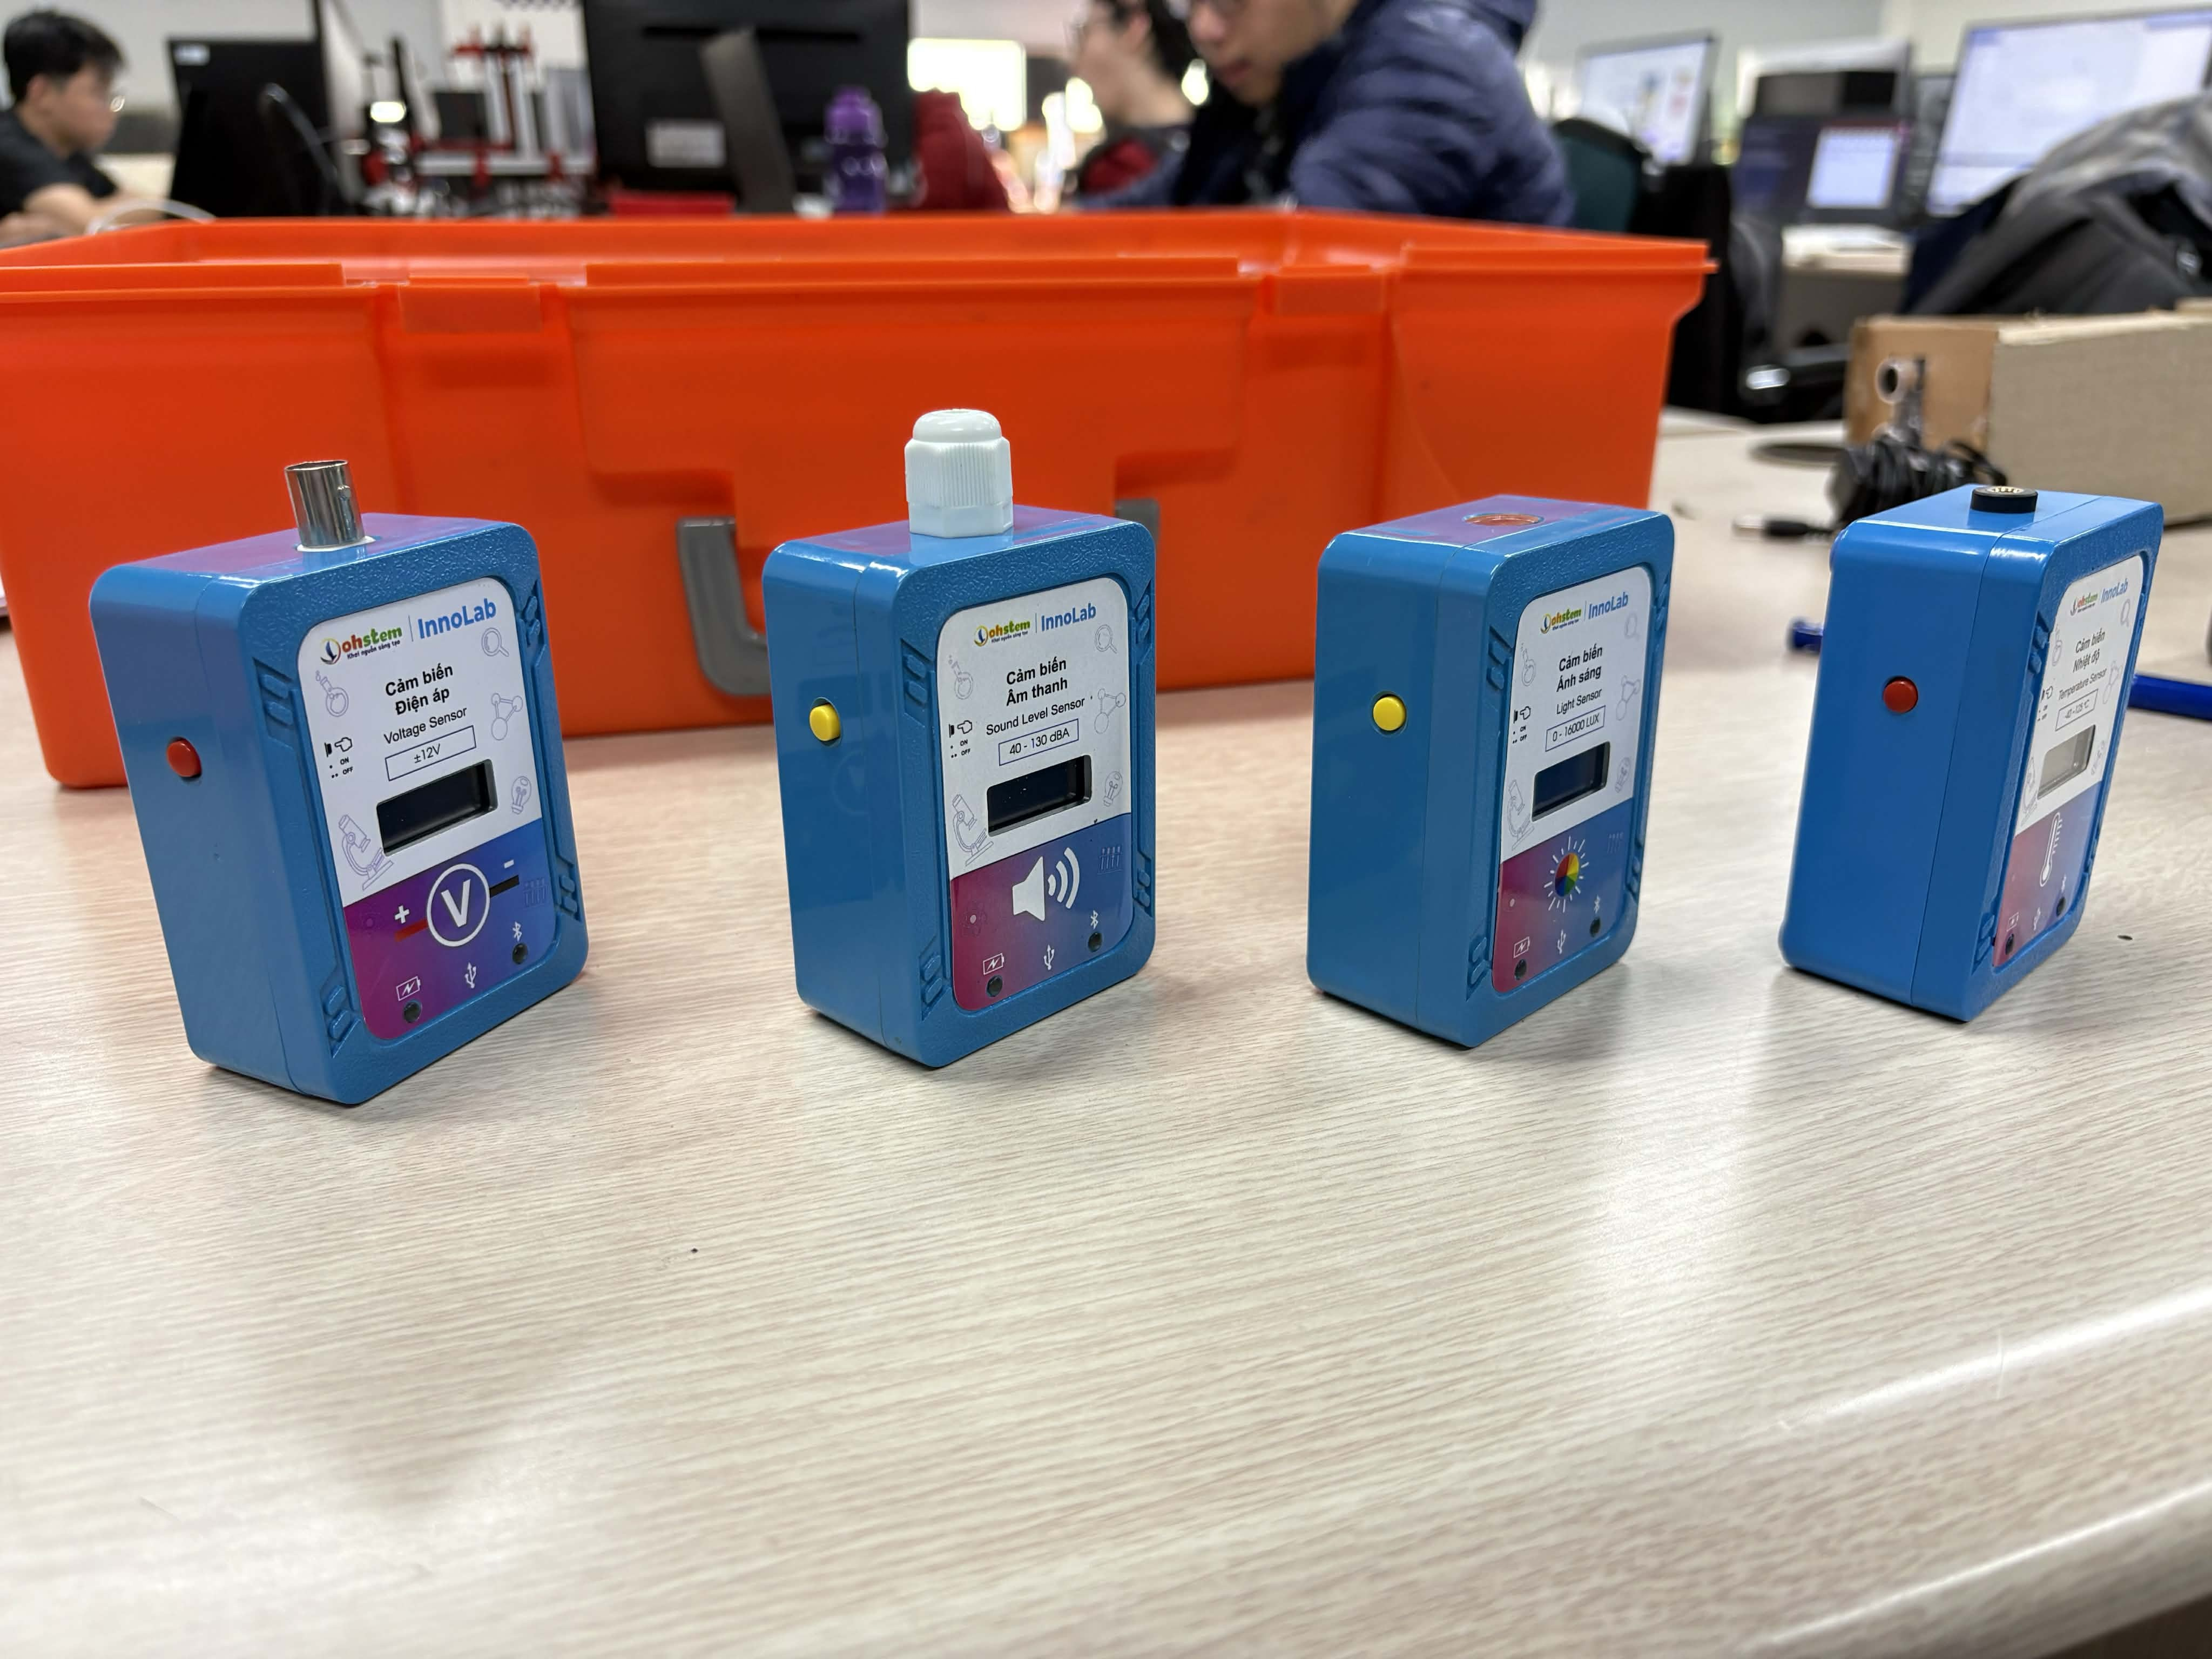
\includegraphics[width=0.5\textwidth]{Images/SimpleModule.jpg}
    \captionsetup{font=small}
    \caption{Ví dụ các module cảm biến đơn chức năng trên thị trường.}
\end{figure}

Để giải quyết các vấn đề trên, đề tài tập trung phát triển một \textbf{hệ thống nhúng chuẩn hóa kết nối và quản lý đa cảm biến} dựa trên vi điều khiển ESP32, ứng dụng mô hình truyền thông không dây \textbf{Wi-Fi Mesh}. Thay vì thiết kế một hệ thống cứng nhắc phục vụ một bài toán duy nhất, dự án cung cấp một bộ giải pháp toàn diện bao gồm cả thiết bị đầu cuối (Node) và bộ thu thập trung tâm (Gateway). Cụ thể, hệ thống cho phép:
\begin{itemize}
    \item Tại các Node cảm biến (MSMS): Người dùng được phép tùy chọn và tự động ánh xạ loại cảm biến muốn sử dụng thông qua hệ thống menu trên màn hình OLED.
    \item Về kết nối mạng: Tích hợp nhiều Node cảm biến thành một mạng \textbf{Wi-Fi Mesh (ESP-Mesh-Lite)} không cần Router định tuyến trung tâm, giúp tự động kết nối và thu thập dữ liệu trên diện rộng.
    \item Tại mạch Gateway: Thu thập, tập hợp dữ liệu từ toàn mạng Mesh, sau đó đồng bộ lên máy chủ (server/backend) qua các giao thức MQTT/WebSocket.
    \item Về giám sát: Dữ liệu được lưu trữ, phân tích và trực quan hóa thời gian thực trên các nền tảng Web Dashboard và Mobile App.
\end{itemize}

Hệ thống vì thế không chỉ là một trạm đo đơn lẻ, mà là một \textbf{giải pháp IoT linh hoạt, toàn diện từ biên đến đám mây}, có thể tái cấu hình cho nhiều bài toán giám sát khác nhau (nhiệt độ–độ ẩm, chất lượng không khí, khí gas, chất lượng nước...) và vận hành bền bỉ trên quy mô lớn.

\subsection{Mục tiêu và phạm vi của dự án}
Mục tiêu cốt lõi của dự án là thiết kế và xây dựng một hệ thống mạng cảm biến phân tán, đảm bảo tính chuẩn hóa linh hoạt tại thiết bị biên, tính ổn định trong truyền thông Mesh và khả năng quản lý tập trung. Cụ thể:
\begin{itemize}
    \item Thiết kế và chuẩn hóa phần cứng/phần mềm cho các thiết bị Node cảm biến (MSMS): Hỗ trợ giao diện chọn cảm biến trực quan qua màn hình, dễ dàng thêm/bớt các loại cảm biến mới mà không cần can thiệp lại mã nguồn.
    \item Triển khai giải pháp \textbf{mạng Wi-Fi Mesh (ESP-Mesh-Lite)} không dùng Router, cho phép các Node tự động kết nối, định tuyến và truyền dữ liệu tầm xa về một điểm tập trung.
    \item Xây dựng thiết bị \textbf{Gateway} để làm cầu nối tiếp nhận dữ liệu từ mạng Mesh, xử lý và đẩy dữ liệu lên máy chủ ứng dụng qua MQTT/WebSocket.
    \item Xây dựng hệ sinh thái phần mềm bao gồm Web Dashboard để giám sát dữ liệu và công cụ Python để đo đạc tải mạng, kiểm thử tỷ lệ Packet Loss.
\end{itemize}

Phạm vi của dự án tập trung vào:
\begin{itemize}
    \item Chế tạo hoàn thiện thiết bị Node cảm biến hỗ trợ cấu hình đa cổng và thiết bị Gateway thu thập dữ liệu mạng Mesh.
    \item Triển khai luồng dữ liệu thông suốt: Cảm biến $\rightarrow$ Node (MSMS) $\rightarrow$ Mạng Wi-Fi Mesh $\rightarrow$ Gateway $\rightarrow$ Server $\rightarrow$ Giao diện Web.
    \item Đo đạc và đánh giá mức độ ổn định của giao thức mạng Mesh khi truyền tải dữ liệu với lưu lượng giả lập lớn.
\end{itemize}

\subsection{Tóm tắt cấu trúc dự án}
Báo cáo dự án ``Xây dựng hệ thống nhúng chuẩn hóa kết nối \& quản lý đa cảm biến'' gồm 5 chương:
\begin{itemize}
    \item \textbf{Chương 1 – Chương mở đầu}: Trình bày bối cảnh, lý do chọn đề tài, mục tiêu, phạm vi và cấu trúc báo cáo.
    \item \textbf{Chương 2 – Phân tích yêu cầu kĩ thuật}: Xác định yêu cầu chức năng, phi chức năng và thiết kế hệ thống tổng thể (Node đa cảm biến, Wi-Fi Mesh, Gateway, Web/App).
    \item \textbf{Chương 3 – Thiết kế chi tiết hệ thống}: Mô tả chuyên sâu về thiết kế mạch phần cứng, firmware cho thiết bị Node, cơ chế hoạt động của ESP-Mesh-Lite và cấu trúc mạch Gateway.
    \item \textbf{Chương 4 – Kiểm thử hệ thống}: Trình bày các kịch bản kiểm thử hoạt động của phần cứng, mô phỏng lưu lượng bằng công cụ Python và đánh giá tỷ lệ hao hụt dữ liệu (Packet Loss) trên mạng Mesh.
    \item \textbf{Chương 5 – Kết luận và hướng phát triển}: Tổng kết kết quả đạt được, đánh giá mức độ đáp ứng mục tiêu và đề xuất các hướng phát triển như tích hợp AI/Cloud nâng cao.
\end{itemize}

\newpage

\section*{CHƯƠNG 2. PHÂN TÍCH YÊU CẦU KĨ THUẬT}
\addcontentsline{toc}{section}{\numberline{}CHƯƠNG 2. PHÂN TÍCH YÊU CẦU KĨ THUẬT}
\label{chuong2}
\setcounter{section}{2}
\setcounter{subsection}{0} % Đặt lại số thứ tự của subsection về 0
% Đặt lại số thứ tự của hình và bảng khi bắt đầu chương mới
\setcounter{figure}{0}
\setcounter{table}{0}

\subsection{Các trường dữ liệu và loại cảm biến}
\label{canguavan}
Để module MSMS có thể tái sử dụng cho nhiều bài toán khác nhau, trước hết cần xác định rõ \textbf{những nhóm trường dữ liệu chính} mà hệ thống phải hỗ trợ, tương ứng với các loại cảm biến được tích hợp. Trong phạm vi đồ án, các nhóm dữ liệu chính được xem xét như sau:

\begin{itemize}
    \item \textbf{Nhóm cảm biến môi trường:}  
    Bao gồm các trường dữ liệu như nhiệt độ, độ ẩm, áp suất không khí, có thể được cung cấp bởi các cảm biến như BME280, DHT22 hoặc các cảm biến tương đương. Đây là nhóm dữ liệu phổ biến trong các ứng dụng giám sát môi trường, nhà thông minh và nông nghiệp thông minh.

    \item \textbf{Nhóm cảm biến chất lượng nước:}  
    Gồm các trường dữ liệu như pH, độ dẫn điện (EC), tổng chất rắn hòa tan (TDS), độ đục, nhiệt độ nước, hàm lượng oxy hòa tan (DO), \dots Nhóm này phù hợp cho các ứng dụng giám sát ao nuôi thủy sản, chất lượng nước sinh hoạt, nước thải công nghiệp hoặc các mô hình thí nghiệm trong phòng lab.

    \item \textbf{Nhóm cảm biến khí và chất lượng không khí:}  
    Gồm các chỉ số như nồng độ CO\textsubscript{2}, khí gas dễ cháy, khói, các khí độc; các giá trị này thường được thể hiện theo đơn vị ppm hoặc µg/m\textsuperscript{3} và có thể mở rộng thêm tuỳ theo loại cảm biến được hỗ trợ.

    \item \textbf{Nhóm dữ liệu mở rộng:}  
    Hệ thống MSMS được thiết kế để có thể bổ sung thêm các loại cảm biến mới (ví dụ cảm biến dòng điện, điện áp, rung động, ánh sáng, \dots) mà không cần thay đổi kiến trúc tổng thể. Mỗi cảm biến mới chỉ cần khai báo thêm tập trường dữ liệu (tên trường, đơn vị, số lượng trường) tương ứng.
\end{itemize}

Ở mức trừu tượng, mỗi loại cảm biến trong hệ thống đều đi kèm với:
\begin{itemize}
    \item Tập các trường dữ liệu mà nó cung cấp (ví dụ: ``nhiệt độ'', ``độ ẩm'', ``pH'', \dots).
    \item Đơn vị đo tương ứng cho từng trường (ví dụ: \textdegree C, \%, ppm, NTU, \dots).
    \item Các giới hạn đo và độ phân giải phù hợp với từng ứng dụng.
\end{itemize}

Với cách phân nhóm như trên, MSMS không bị ràng buộc vào một loại cảm biến cố định mà có thể mở rộng dần danh sách cảm biến hỗ trợ, miễn là mô tả được các trường dữ liệu và đơn vị đo tương ứng.

\subsection{Tốc độ lấy mẫu và giới hạn truyền dữ liệu}
\label{tocdo}
Để đảm bảo hệ thống không bị mất mát dữ liệu khi nhiều node MSMS gửi đồng thời về gateway, cần phân tích và giới hạn tốc độ lấy mẫu, kích thước gói tin cũng như băng thông tổng hợp tại mạch gateway.
\subsubsection{Tốc độ lấy mẫu tại node MSMS}
Mỗi node MSMS có thể trang bị tối đa 3 cổng cảm biến, mỗi cổng một loại cảm biến. Tần suất lấy mẫu điển hình của một số cảm biến được hỗ trợ trong hệ thống:
\begin{table}[H]
    \centering
    \caption{Tần suất lấy mẫu và số trường dữ liệu của các cảm biến hỗ trợ}
    \label{tab:sensor_rate}
    \renewcommand{\arraystretch}{1.3}
    \makebox[\textwidth][c]{%
    \begin{tabular}{|l|c|c|c|}
    \hline
    \textbf{Cảm biến} & \textbf{Tần suất tối đa} & \textbf{Tần suất khuyến nghị} & \textbf{Số trường dữ liệu} \\
    \hline
    BME280 & 157.5 Hz & 1 Hz & 3 (nhiệt độ, độ ẩm, áp suất) \\
    DHT22 & 0.5 Hz & 0.5 Hz & 2 (nhiệt độ, độ ẩm) \\
    MH-Z14A (CO\textsubscript{2}) & 1 Hz & 0.2 Hz & 1 (CO\textsubscript{2} ppm) \\
    MQ-2, MQ-135 & 10 Hz & 1 Hz & 1 (nồng độ khí) \\
    PMS7003 & 1 Hz & 0.2 Hz & 3 (PM1.0, PM2.5, PM10) \\
    \dots & \dots & \dots & \dots \\
    \hline
    \end{tabular}%
    }
\end{table}
Trong thực tế, tần suất lấy mẫu khuyến nghị cho toàn hệ thống là \textbf{1 lần/giây (1~Hz)} với các cảm biến thông thường và \textbf{0.2~Hz} với các cảm biến cần ổn định lâu như MH-Z14A, PMS7003. Mỗi bản ghi gửi lên gateway được đóng gói dưới định dạng chuỗi JSON (UTF-8, compact) với cấu trúc như sau:
\begin{itemize}
    \item \textbf{Metadata:} Bao gồm schema version (\texttt{v}), sequence counter (\texttt{seq}), mesh level (\texttt{n}), IPv4 (\texttt{i}), thời gian RTC (\texttt{t}), version (\texttt{ver}), và mã lỗi (\texttt{err}) -- chiếm khoảng 100~byte.
    \item \textbf{Payload (\texttt{p}):} Chứa mảng dữ liệu của các cổng cảm biến, với mỗi cổng mang thông tin \texttt{[port, type, val1, val2, ...]} -- chiếm từ 15 đến 30~byte mỗi cổng.
\end{itemize}
Với cấu hình tối đa 3 cổng cảm biến đồng thời, kích thước một gói tin điển hình dao động từ \textbf{130 đến 200~byte}.
\subsubsection{Tốc độ truyền qua Wi-Fi Mesh và xử lý tại Root - Gateway}
Giao tiếp giữa các node MSMS và mạch Root sử dụng ESP-Mesh-Lite trên Wi-Fi 802.11n (2.4~GHz). Băng thông lý thuyết tối đa đạt 72.2~Mbps (single stream MCS7), tuy nhiên trong môi trường mesh thực tế, mỗi hop trung gian làm giảm throughput và tăng độ trễ do phải nhận rồi chuyển tiếp gói tin trên cùng một kênh vô tuyến. Mạch Root đóng vai trò đầu cuối tập trung toàn bộ luồng dữ liệu từ mọi node MSMS. Sau đó, mạch Root chuyển tiếp luồng dữ liệu này sang mạch Gateway thông qua kết nối nối tiếp UART. Mạch Gateway sẽ chịu trách nhiệm xử lý CPU cường độ cao (parse JSON, ghi SD card, kết nối server và gửi MQTT/WebSocket). Các thông số truyền dữ liệu Mesh thực tế được tóm tắt trong bảng~\ref{tab:mesh_rate}.
\begin{table}[H]
    \centering
    \caption{Thông số truyền dữ liệu trong mạng Wi-Fi Mesh (ESP-Mesh-Lite)}
    \label{tab:mesh_rate}
    \renewcommand{\arraystretch}{1.3}
    \begin{tabular}{|l|c|}
    \hline
    \textbf{Thông số} & \textbf{Giá trị} \\
    \hline
    Chuẩn Wi-Fi & 802.11b/g/n (2.4~GHz) \\
    Throughput ứng dụng thực tế (1 hop) & 1--5~Mbps \\
    Độ trễ mỗi hop & 10--50~ms \\
    Kích thước gói MSMS điển hình & 130--200~byte \\
    Số node tối đa mỗi lớp (ESP-Mesh-Lite) & lên đến 10~node \\
    Giao thức lớp ứng dụng & TCP/UDP (socket) \\
    \hline
    \end{tabular}
\end{table}
\subsubsection{Phân tích và tính toán giới hạn tốc độ toàn hệ thống}
Để đảm bảo hệ thống hoạt động ổn định và không bị rớt gói tin (packet loss), băng thông tại mỗi chặng truyền dữ liệu phải lớn hơn hoặc bằng tổng lưu lượng do toàn bộ các node cảm biến sinh ra. Giả sử hệ thống có $N$ node MSMS, mỗi node gửi $f$ gói/giây với kích thước $S$~byte. Tổng lưu lượng sinh ra là:
\[
R_{\text{total}} = N \times f \times S \times 8 \quad \text{(bit/s)}
\]
Luồng dữ liệu đi qua hai chặng chính: (1) từ các node qua mạng Wi-Fi Mesh truyền về mạch Root, và (2) từ mạch Root qua giao tiếp UART đẩy sang mạch Gateway.

\textbf{Chặng 1: Giới hạn của mạng Wi-Fi Mesh}\\
Gọi $R_{\text{mesh\_rx}}$ là băng thông nhận ứng dụng thực tế tối đa mà mạch Root có thể xử lý từ mạng Wi-Fi ESP-Mesh-Lite. Lấy $R_{\text{mesh\_rx}} \approx 1~\text{Mbps}$ (mức an toàn qua 1 hop mesh). Để không nghẽn tại chặng này, cần $R_{\text{total}} \leq R_{\text{mesh\_rx}}$. Với $S = 200$~byte, $f = 1$~Hz, số node tối đa mạch Root gánh được trên mạng Mesh là:
\[
N_{\text{mesh}} = \frac{R_{\text{mesh\_rx}}}{f \times S \times 8} = \frac{1{,}000{,}000}{1 \times 200 \times 8} = 625 \text{ node}
\]

\textbf{Chặng 2: Giới hạn của giao tiếp UART (Root $\rightarrow$ Gateway)}\\
Giả sử giao tiếp UART được cấu hình ở tốc độ baud rate là $B$ (bps). Với khung truyền chuẩn 8N1 (1 start bit, 8 data bits, 1 stop bit), mỗi byte dữ liệu cần 10 bit để truyền tải. Số gói tin tối đa UART truyền được trong một giây (với kích thước $S = 200$~byte) là $P_{\text{UART}} = \frac{B}{10 \times S}$. Số node tối đa đáp ứng được qua UART (ứng với $f = 1$~Hz) là:
\[
N_{\text{uart}} = P_{\text{UART}} = \frac{B}{2000} \text{ node}
\]
Dựa vào tốc độ baud, ta có các kịch bản:
\begin{itemize}
    \item \textbf{115,200 bps}: $N_{\text{uart}} \approx \textbf{57 node}$. UART trở thành điểm nghẽn nghiêm trọng, làm lãng phí băng thông Mesh và dễ gây tràn hàng đợi (queue overflow) tại Root.
    \item \textbf{921,600 bps}: $N_{\text{uart}} \approx \textbf{460 node}$. Đáp ứng được phần lớn các mạng IoT quy mô trung bình.
    \item \textbf{1,500,000 bps}: $N_{\text{uart}} = \textbf{750 node}$. Tốc độ UART hoàn toàn vượt qua khả năng thu thập của Mesh ($750 > 625$), giải phóng triệt để điểm nghẽn.
\end{itemize}

\textbf{Kết luận về giới hạn lý thuyết}\\
Sức chứa lý thuyết tối đa của toàn hệ thống được quyết định bởi điểm thắt cổ chai hẹp nhất giữa hai chặng:
\[
N_{\text{max}} = \min(N_{\text{mesh}}, N_{\text{uart}})
\]
Như vậy, để hệ thống có thể phát huy tối đa giới hạn 625 node của mạng ESP-Mesh-Lite, kết nối UART buộc phải thiết lập ở tốc độ từ \textbf{1,250,000 bps trở lên}. 

Tuy nhiên, giới hạn tổng thể của hệ thống thực tế không chỉ nằm ở mạng Mesh hay UART, mà còn phụ thuộc vào khả năng chịu tải CPU của mạch Gateway khi phân tích chuỗi JSON và tốc độ ghi thẻ SD card (giới hạn ở mức 1--4~MB/s cho FAT32). Do đó, giới hạn an toàn thực tế thấp hơn nhiều so với khả năng truyền tải lý thuyết. Bảng~\ref{tab:rate_limit} đưa ra các ngưỡng an toàn khuyến nghị cho hệ thống:
\begin{table}[H]
    \centering
    \caption{Giới hạn tốc độ khuyến nghị để đảm bảo không mất mát dữ liệu}
    \label{tab:rate_limit}
    \renewcommand{\arraystretch}{1.3}
    \begin{tabular}{|l|c|c|}
    \hline
    \textbf{Tham số} & \textbf{Giới hạn khuyến nghị} & \textbf{Giới hạn tối đa} \\
    \hline
    Số node MSMS & $\leq 10$ node & 20 node \\
    Tần suất gửi mỗi node & 1 lần/giây & 5 lần/giây \\
    Kích thước gói mỗi bản ghi & $\leq 512$~byte & 1024~byte \\
    Tổng lưu lượng đến gateway & $\leq 50$~Kbps & 200~Kbps \\
    Số hop tối đa trong mesh & 3 hop & 5 hop \\
    \hline
    \end{tabular}
\end{table}
Trong phạm vi đồ án, hệ thống được kiểm thử với \textbf{2 node MSMS} và 1 mạch gateway, tần suất gửi 1~Hz với gói tin khoảng 200~byte, tổng lưu lượng chỉ khoảng 3.2~Kbps — hoàn toàn nằm trong ngưỡng an toàn. Firmware node MSMS tích hợp cơ chế đệm dữ liệu tạm thời trong RAM khi mất kết nối mesh và gửi lại khi kết nối được phục hồi, đảm bảo không mất mát dữ liệu trong điều kiện mạng không ổn định.

\subsection{Yêu cầu chức năng}
\label{yeucauchucnang}
Từ mục tiêu đề tài đã trình bày ở Chương~1, các yêu cầu chức năng chính của toàn bộ hệ thống có thể được phân chia theo từng thành phần như sau:

\begin{itemize}
    \item \textbf{Tại các Node cảm biến (MSMS):}
    \begin{itemize}
        \item \textbf{Quản lý và cấu hình cảm biến trực tiếp:} Hệ thống cần quản lý danh sách các loại cảm biến được hỗ trợ. Người dùng phải có thể chọn và cấu hình loại cảm biến gắn trên tối đa 3 cổng thông qua menu OLED bằng 3 nút bấm (BACK, SELECT, MOVE), không cần nạp lại code.
        \item \textbf{Thu thập và hiển thị:} Tự động đọc dữ liệu theo chu kỳ, hiển thị kết quả (giá trị, đơn vị) cùng các trạng thái cơ bản (Wi-Fi, mức pin) lên màn hình OLED.
        \item \textbf{Tự động gia nhập mạng Mesh:} Các node phải tự động dò tìm, kết nối và định tuyến với nhau để hình thành mạng Wi-Fi ESP-Mesh-Lite mà không cần Router trung tâm.
    \end{itemize}
    
    \item \textbf{Tại Root Node và Gateway:}
    \begin{itemize}
        \item \textbf{Tập hợp dữ liệu:} Mạch Root đóng vai trò là đỉnh của mạng Mesh, có nhiệm vụ tiếp nhận toàn bộ gói tin từ các node con và truyền sang mạch Gateway qua cổng UART tốc độ cao.
        \item \textbf{Đồng bộ hóa thời gian và lưu trữ:} Cập nhật thời gian thực qua RTC và lưu trữ dự phòng dữ liệu toàn mạng vào thẻ SD Card.
        \item \textbf{Giao tiếp Server:} Mạch Gateway xử lý phân tích gói tin JSON, sau đó đẩy dữ liệu lên hệ thống máy chủ thông qua giao thức WebSocket và MQTT.
    \end{itemize}
    
    \item \textbf{Tại hệ thống quản lý (Dashboard \& Mobile App):}
    \begin{itemize}
        \item \textbf{Giám sát thời gian thực:} Hiển thị dữ liệu đo đạc (nhiệt độ, độ ẩm, nồng độ khí...) của tất cả các node trong mạng Mesh một cách trực quan trên Web (React) và ứng dụng di động (React Native).
    \end{itemize}
\end{itemize}

\subsection{Yêu cầu phi chức năng}
\label{yeucauphichucnang}
Bên cạnh các yêu cầu chức năng, hệ thống cần đáp ứng các yêu cầu phi chức năng (Non-functional Requirements) khắt khe để đảm bảo khả năng triển khai thực tế:

\begin{itemize}
    \item \textbf{Tính ổn định và tự phục hồi của mạng Mesh (Self-healing):}  
    Mạng ESP-Mesh-Lite phải có khả năng tự động cấu hình lại (re-routing) khi một node trung gian mất kết nối. Dữ liệu tại các node cần được lưu đệm tạm thời vào RAM để gửi bù sau khi mạng kết nối lại, đảm bảo tính nguyên vẹn của dữ liệu thu thập.

    \item \textbf{Hiệu năng xử lý không thắt cổ chai (Bottleneck-free):}  
    Hệ thống phải duy trì tính liền mạch trong suốt luồng dữ liệu từ Node $\rightarrow$ Root $\rightarrow$ Gateway. Tốc độ giao tiếp UART giữa Root và Gateway phải được thiết lập tối thiểu 921,600 bps để xả kịp lượng dữ liệu lớn đổ về từ mạng Mesh.

    \item \textbf{Tính linh hoạt và tái sử dụng (Modularity):}  
    Cấu trúc firmware cần được module hóa mạnh mẽ (đặc biệt là lớp cấu hình cảm biến) để việc tích hợp thêm một loại cảm biến mới trong tương lai chỉ yêu cầu bổ sung cấu hình mà không phá vỡ logic giao diện hoặc giao thức mạng.

    \item \textbf{Hiệu suất giao diện cục bộ:}  
    Thời gian phản hồi trên màn hình OLED tại các node khi nhấn nút phải đảm bảo độ mượt mà (debounce tốt, không block CPU), ngay cả khi thiết bị đang bận xử lý gửi dữ liệu qua mạng Mesh.

    \item \textbf{Tiêu thụ năng lượng và độ bền bỉ:}  
    Các module cần được trang bị hệ thống quản lý nguồn thông minh, tự động chuyển đổi giữa nguồn adapter và nguồn pin (power path management) để hệ thống không bao giờ bị gián đoạn hoạt động, đảm bảo độ tin cậy trong giám sát dài hạn.
\end{itemize}

\newpage
\section*{CHƯƠNG 3. THIẾT KẾ CHI TIẾT HỆ THỐNG}
\addcontentsline{toc}{section}{\numberline{}CHƯƠNG 3. THIẾT KẾ CHI TIẾT HỆ THỐNG}
\setcounter{section}{3}
\setcounter{subsection}{0}
\setcounter{figure}{0}
\setcounter{table}{0}
Từ những yêu cầu chức năng và phi chức năng đã xác định ở phần~\hyperref[chuong2]{CHƯƠNG 2}, ta sẽ bắt đầu tiến hành thiết kế chi tiết hệ thống
của dự án này. Toàn bộ chương 3 này sẽ trình bày thiết kế hardware, firmware từ tổng quan đến chi tiết.
\subsection{Thiết kế tổng thể hệ thống}
\subsubsection{Tổng quan và sơ đồ hệ thống} 
\begin{figure}[H]
    \centering
    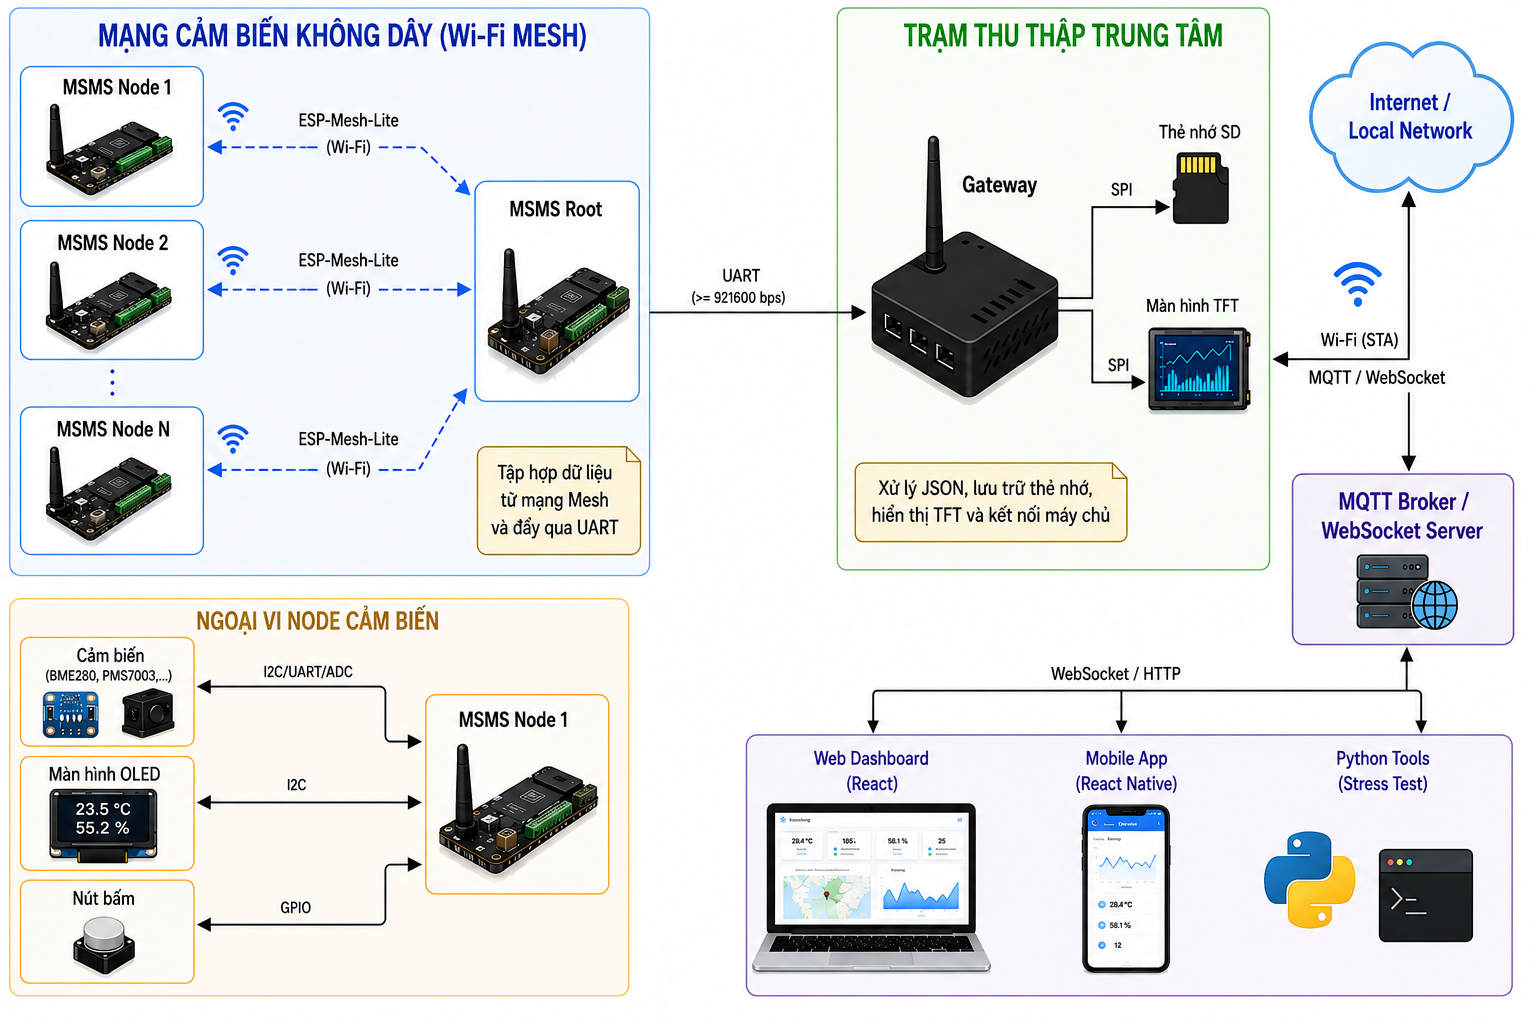
\includegraphics[width=1.0\textwidth]{Images/SoDoHeThong.png}
    \captionsetup{font=small}  % Chỉnh kích thước chữ caption nhỏ
    \caption{Cấu trúc tổng quan của hệ thống.}
\end{figure}

Hình 3.1 minh họa sơ đồ kiến trúc tổng quan của toàn bộ hệ thống Wi-Fi Mesh Sensor Monitoring System. Khác với một module đo đạc đơn lẻ, dự án được thiết kế phân lớp rõ ràng nhằm giải quyết bài toán thu thập dữ liệu ở quy mô lớn. Hệ thống bao gồm 4 phân lớp chính:

\textbf{1. Lớp Ngoại vi và Node Cảm biến (MSMS Nodes):}
\begin{itemize}
    \item Mỗi node là một thiết bị ESP32 độc lập, được trang bị các cổng cắm module cảm biến (BME280, PMS7003, MQ-135...) giao tiếp qua I2C/UART/ADC.
    \item Để phục vụ nhu cầu thao tác tại chỗ, mỗi node có một màn hình OLED SSD1306 (độ phân giải 128$\times$64, giao tiếp I2C) để hiển thị thông số và một hệ thống 3 nút bấm cơ học (BACK, SELECT, MOVE) để người dùng điều hướng menu, cấu hình thiết bị trực tiếp mà không cần nạp lại phần mềm.
    \item Toàn bộ node được duy trì hoạt động thông qua \textbf{hệ thống quản lý nguồn} thông minh gồm pin Lithium, mạch sạc/boost có hỗ trợ power path management (chuyển mạch không sập nguồn), và mạch buck hạ áp 3.3V cấp cho vi điều khiển.
\end{itemize}

\textbf{2. Lớp Mạng cảm biến không dây (Wi-Fi Mesh):}
\begin{itemize}
    \item Các MSMS Node tự động kết nối với nhau để hình thành một mạng lưới không dây sử dụng giao thức ESP-Mesh-Lite.
    \item Mạng lưới này cho phép các node ở xa truyền tiếp (hop) dữ liệu qua các node trung gian, cuối cùng đổ dồn toàn bộ gói tin về một node trung tâm duy nhất gọi là \textbf{MSMS Root}.
\end{itemize}

\textbf{3. Lớp Trạm thu thập trung tâm (Gateway):}
\begin{itemize}
    \item Lớp này bao gồm 2 vi điều khiển ghép nối với nhau: MSMS Root và Gateway.
    \item \textbf{MSMS Root} chỉ đóng vai trò duy trì mạng Mesh và gom dữ liệu. Sau khi nhận dữ liệu từ các node, mạch Root đẩy toàn bộ sang mạch Gateway thông qua kết nối dây nối tiếp \textbf{UART} ở tốc độ rất cao ($\ge$ 921,600 bps) để tránh nghẽn cổ chai.
    \item \textbf{Mạch Gateway} đóng vai trò như một máy chủ xử lý dữ liệu ở vùng biên (edge server). Nó phân tích chuỗi JSON nhận được, đóng dấu thời gian từ module RTC DS3231 (giao tiếp I2C), sau đó thực hiện 3 nhiệm vụ song song: 
    (1) Lưu trữ dự phòng dữ liệu toàn mạng vào thẻ nhớ \textbf{SD Card} (giao tiếp SPI). 
    (2) Hiển thị thông số tổng hợp lên \textbf{màn hình TFT} (giao tiếp SPI) phục vụ người giám sát trạm.
    (3) Đóng gói và truyền lên đám mây.
\end{itemize}

\textbf{4. Lớp Đám mây và Hệ thống giám sát (Internet \& Clients):}
\begin{itemize}
    \item Mạch Gateway kết nối Internet thông qua Wi-Fi ở chế độ trạm (STA) và truyền dữ liệu JSON tới hệ thống máy chủ thông qua giao thức \textbf{MQTT} hoặc \textbf{WebSocket}.
    \item Dữ liệu từ Server sau đó được phân phối theo thời gian thực tới các nền tảng khách hàng (Clients) bao gồm: \textbf{Web Dashboard} (xây dựng bằng React), \textbf{Mobile App} (xây dựng bằng React Native), và các script Python (dùng để stress test hoặc trích xuất số liệu phân tích).
\end{itemize}

Cách phân lớp này giúp hệ thống vừa đảm bảo khả năng thu thập dữ liệu rải rác ngoài thực địa, vừa giảm tải xử lý cho mạch Mesh trung tâm, đồng thời cung cấp được đa dạng phương thức giám sát từ cục bộ (OLED/TFT) đến toàn cầu (Web/App).
\subsubsection{Linh kiện sử dụng}

\begin{enumerate}[label=\alph*), leftmargin=1.5cm, itemsep=15pt]
    \item \phantomsection
    \addcontentsline{toc}{paragraph}{A) Vi điều khiển ESP32}
    \textbf{Vi điều khiển ESP32}

    ESP32 là một dòng vi điều khiển tích hợp module Wi-Fi và Bluetooth hiệu suất cao, giá thành thấp, được sản xuất bởi Espressif Systems. Với khả năng xử lý mạnh mẽ, ESP32 phù hợp cho các ứng dụng IoT, đặc biệt là các ứng dụng yêu cầu khả năng giao tiếp không dây mạnh mẽ và đáng tin cậy.
    \begin{table}[H]
        \centering
        \caption{Thông số kỹ thuật ESP32}
        \label{tab:esp32}
        \renewcommand{\arraystretch}{1.3}
        \begin{tabular}{|l|l|}
        \hline
        \textbf{Thông số} & \textbf{Giá trị} \\
        \hline
        Vi xử lý & Xtensa® Dual-Core 32-bit LX6 \\
        Xung nhịp & 160 MHz (tối đa 240 MHz) \\
        Wi-Fi & 802.11 b/g/n (2.4 GHz) \\
        Bluetooth & Bluetooth 4.2 + BLE \\
        RAM & 520 KB SRAM \\
        Flash & Tối đa 16 MB (ngoài) \\
        GPIO & Tối đa 34 chân \\
        ADC & 12-bit, 18 kênh \\
        Điện áp hoạt động & 3.3 V \\
        \hline
        \end{tabular}
    \end{table}

    \begin{figure}[H]
        \centering
        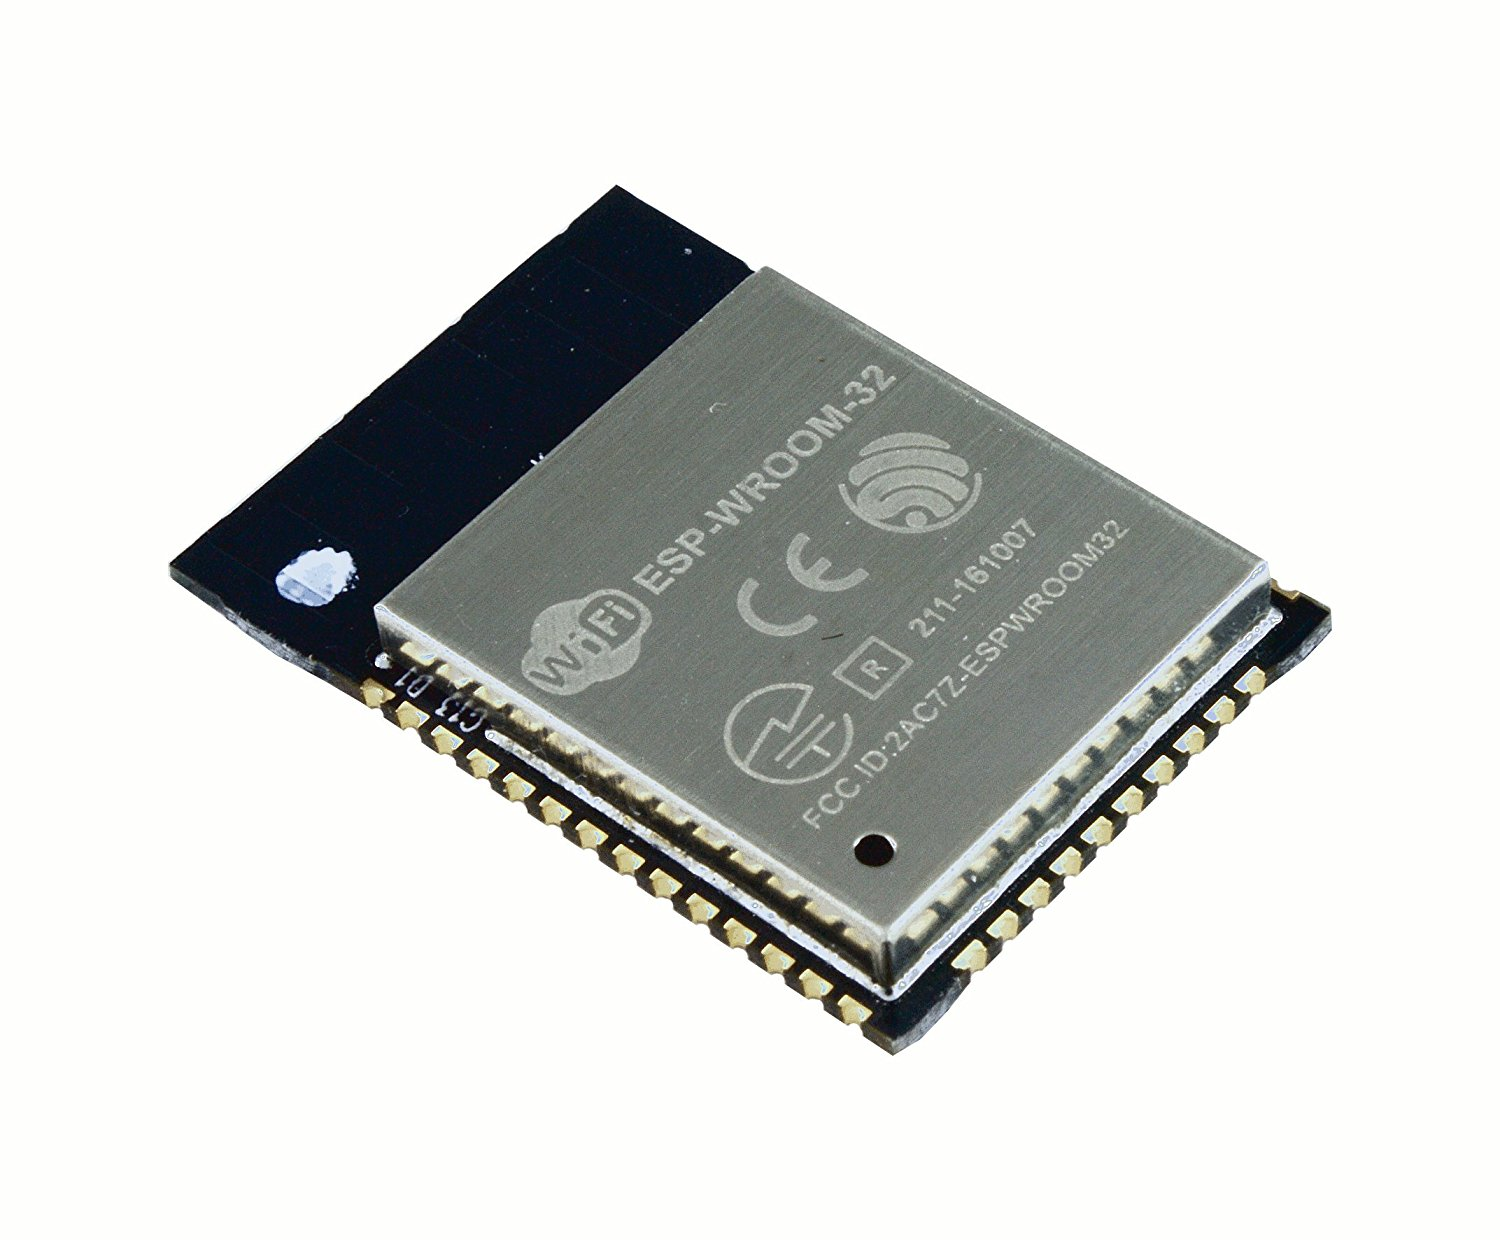
\includegraphics[width=0.4\textwidth]{Images/ESP32WR.jpg}
        \captionsetup{font=small}  % Chỉnh kích thước chữ caption nhỏ
        \caption{Vi điều khiển ESP32.}
    \end{figure}


    
    \item \phantomsection
    \addcontentsline{toc}{paragraph}{B) Module RTC DS3231}
    \textbf{Module RTC DS3231}

    DS3231 là một module đồng hồ thời gian thực (RTC) có độ chính xác cao, sử dụng dao động thạch anh tích hợp bên trong và bộ bù nhiệt độ. Nó cho phép đo thời gian chính xác đến từng giây, có pin dự phòng nên vẫn hoạt động trong điều kiện mất nguồn. DS3231 hỗ trợ giao tiếp I2C và thường được sử dụng trong các ứng dụng cần hẹn giờ, lưu trữ log theo thời gian thực.

    \begin{table}[H]
        \centering
        \caption{Thông số kỹ thuật DS3231}
        \label{tab:ds3231}
        \renewcommand{\arraystretch}{1.3}
        \begin{tabular}{|l|l|}
        \hline
        \textbf{Thông số} & \textbf{Giá trị} \\
        \hline
        Chức năng & Real-Time Clock (RTC) \\
        Độ chính xác & $\pm$2 ppm \\
        Giao tiếp & I2C \\
        Điện áp hoạt động & 2.3 -- 5.5 V \\
        Pin dự phòng & CR2032 \\
        Dòng tiêu thụ & $\sim$3 $\mu$A (backup) \\
        Bộ dao động & TCXO tích hợp \\
        Nhiệt độ hoạt động & -40°C đến +85°C \\
        \hline
        \end{tabular}
        \end{table}

    \begin{figure}[H]
        \centering
        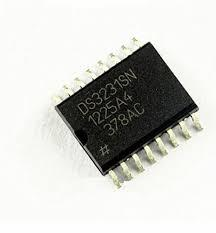
\includegraphics[width=0.5\textwidth]{Images/DS3231.jpg}
        \captionsetup{font=small}  % Chỉnh kích thước chữ caption nhỏ
        \caption{Module DS3231.}
    \end{figure}

    \item \phantomsection
    \addcontentsline{toc}{paragraph}{C) Module lưu trữ SD Card}
    \textbf{Module lưu trữ SD Card}

    SD Card là một giải pháp lưu trữ ngoài tiện lợi, thường được sử dụng trong các hệ thống nhúng để lưu dữ liệu một cách lâu dài và đáng tin cậy.

    SD Card được giao tiếp với vi điều khiển thông qua chuẩn SPI – một giao tiếp nối tiếp tốc độ cao, dễ tích hợp và tương thích với cả ESP32 lẫn STM32.
    \begin{table}[H]
        \centering
        \caption{Thông số kỹ thuật thẻ nhớ SD}
        \label{tab:sdcard}
        \renewcommand{\arraystretch}{1.3}
        \begin{tabular}{|l|l|}
        \hline
        \textbf{Thông số} & \textbf{Giá trị} \\
        \hline
        Chuẩn thẻ & MicroSD \\
        Giao tiếp & SPI \\
        Điện áp hoạt động & 3.3 V \\
        Dung lượng hỗ trợ & Tối đa 32 GB (FAT32) \\
        Dòng tiêu thụ & 50 -- 100 mA \\
        Ứng dụng & Lưu trữ dữ liệu cảm biến \\
        \hline
        \end{tabular}
        \end{table}
    \begin{figure}[H]
        \centering
        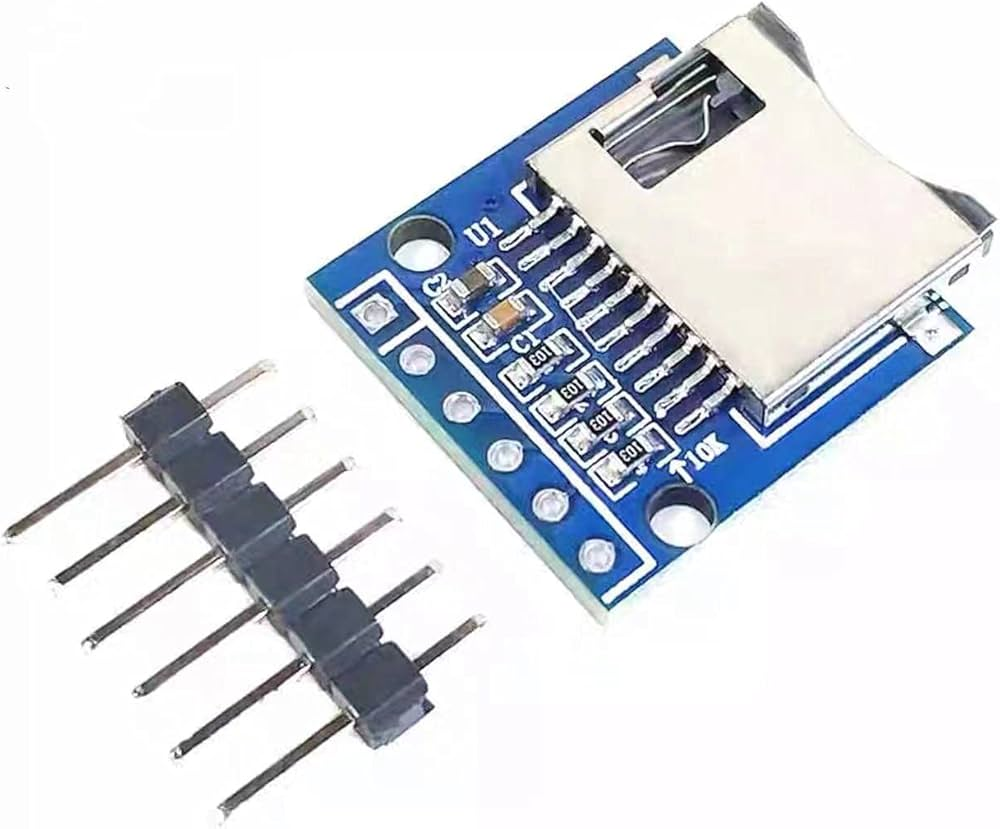
\includegraphics[width=0.5\textwidth]{Images/SdCard.jpg}
        \captionsetup{font=small}  % Chỉnh kích thước chữ caption nhỏ
        \caption{Module SD Card.}
    \end{figure}

    \item \phantomsection
    \addcontentsline{toc}{paragraph}{D) Module mạch sạc IP5306}
    \textbf{Module mạch sạc IP5306}

    IP5306 là một module quản lý nguồn tích hợp được thiết kế để sạc pin lithium và cung cấp đầu ra 5V cho các ứng dụng di động và thiết bị nhúng. Module này tích hợp các chức năng sạc pin, boost converter và power path management trong một chip duy nhất, giúp đơn giản hóa thiết kế mạch nguồn và tối ưu hiệu suất sử dụng pin.

    Module IP5306 hoạt động như một hệ thống quản lý nguồn thông minh với khả năng tự động chuyển đổi giữa chế độ sạc và xả. Khi có nguồn ngoài qua cổng USB Type-C, module sẽ tự động sạc pin và đồng thời cấp nguồn cho tải thông qua tính năng power path management. Khi không có nguồn ngoài, module sẽ sử dụng năng lượng từ pin và boost lên 5V để cấp cho hệ thống.

    \begin{table}[H]
        \centering
        \caption{Thông số kỹ thuật IP5306}
        \label{tab:ip5306}
        \renewcommand{\arraystretch}{1.3}
        \begin{tabular}{|l|l|}
        \hline
        \textbf{Thông số} & \textbf{Giá trị} \\
        \hline
        Chức năng & Quản lý nguồn, sạc pin, boost converter \\
        Điện áp đầu vào & 5 -- 5.5 V \\
        Điện áp cắt sạc & 4.2 V / 4.35 V ($\pm$0.5\%) \\
        Dòng sạc & 2.4 A ($\pm$5\%) \\
        Điện áp đầu ra & 5.0 -- 5.15 V (bù tổn thất dây) \\
        Dòng đầu ra tối đa & 2 A \\
        Độ gợn sóng đầu ra & 100 mV \\
        Hiệu suất chuyển đổi & 92.5\% (đầu vào 3.6V, đầu ra 5V@2A) \\
        Điện áp sạc trước & 2.8 V (dòng 180 mA) \\
        Điện áp sạc lại & 4.1 V \\
        Dòng cắt tự động & 100 mA (sau khi đạt điện áp phao) \\
        Dòng tắt đầu ra & < 50 mA (liên tục) \\
        \hline
        \end{tabular}
        \end{table}
    \begin{figure}[H]
        \centering
        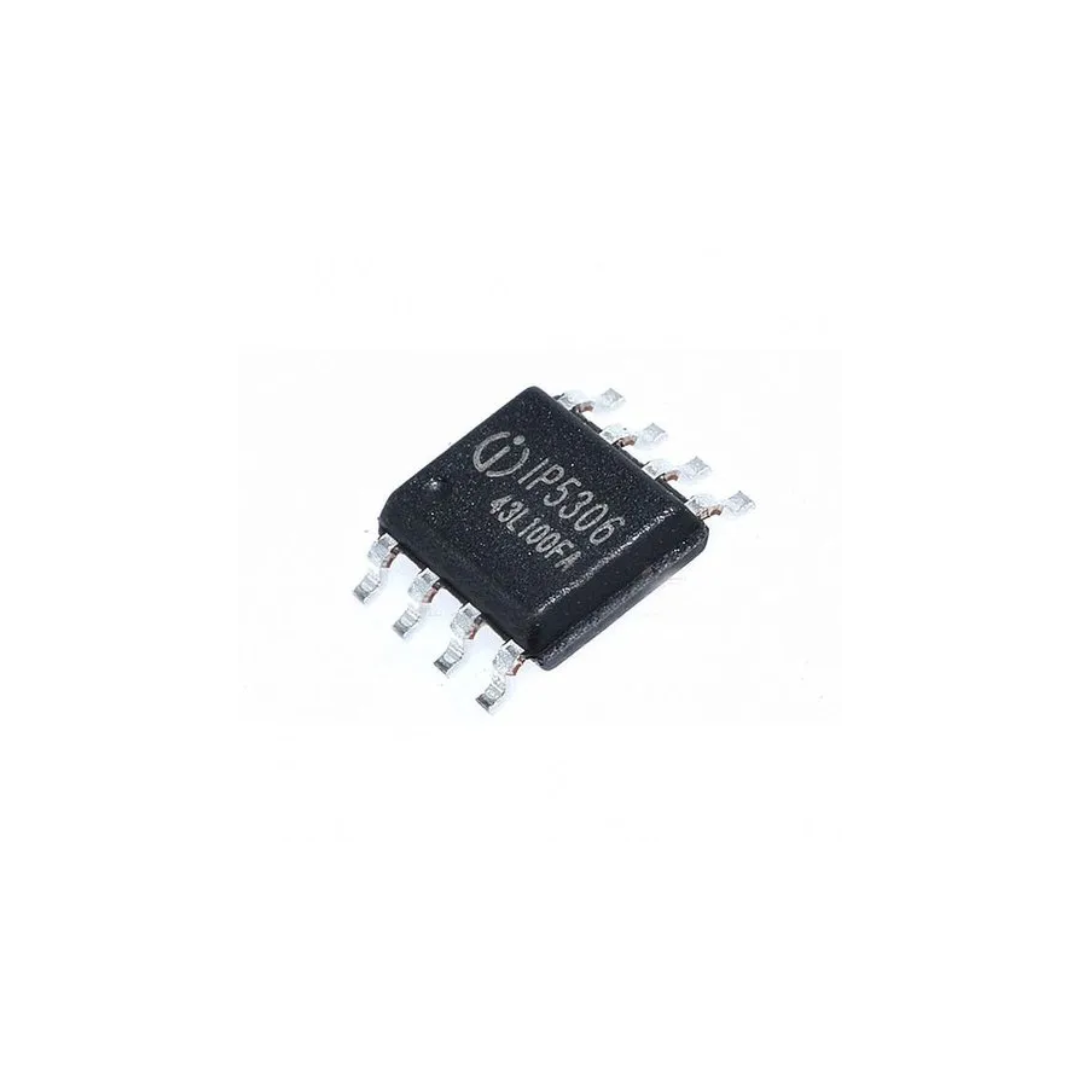
\includegraphics[width=0.5\textwidth]{Images/ip5306.png}
        \captionsetup{font=small}  % Chỉnh kích thước chữ caption nhỏ
        \caption{Module mạch sạc IP5306.}
    \end{figure}
    
    
    Module IP5306 có các đặc điểm nổi bật sau:

    \begin{itemize}
        \item \textbf{Tự động tắt đầu ra khi tải thấp:} Khi dòng tải liên tục nhỏ hơn 50mA, đầu ra sẽ tự động bị tắt để tiết kiệm năng lượng pin.
        
        \item \textbf{Hỗ trợ điều khiển bằng nút bấm ngoài:} Module hỗ trợ kết nối nút bấm với điểm K và đầu ra âm. Nhấn nhanh một lần để bật màn hình hiển thị nguồn và bật đầu ra 5V; nhấn hai lần ngắn liên tiếp để tắt màn hình hiển thị và tắt đầu ra 5V.
        
        \item \textbf{Quản lý chu kỳ sạc thông minh:} Khi dòng sạc giảm xuống 100mA sau khi đạt đến điện áp phao cuối cùng, chu kỳ sạc sẽ tự động kết thúc. Khi điện áp pin giảm dưới 4.1V, chu kỳ sạc lại sẽ tự động bắt đầu.
        
        \item \textbf{Bảo vệ pin điện áp thấp:} Khi điện áp pin thấp hơn 2.8V, pin sẽ được sạc trước với dòng điện 180mA để đảm bảo an toàn và kéo dài tuổi thọ pin.
        
        \item \textbf{Tích hợp cổng USB-A:} Vị trí hàn ổ cắm USB-A cái được cung cấp ở mặt sau của module, cho phép người dùng tự lắp đặt để có đầu ra USB-A tiêu chuẩn phục vụ các ứng dụng khác nhau.
        
        \item \textbf{Hiển thị trạng thái bằng LED:} Module tích hợp 4 đèn LED để hiển thị trạng thái nguồn, mức pin và trạng thái sạc/xả, giúp người dùng dễ dàng theo dõi tình trạng hệ thống.
    \end{itemize}

    Trong hệ thống MSMS, module IP5306 đóng vai trò là khối quản lý nguồn chính, đảm bảo hệ thống có thể hoạt động độc lập với pin lithium trong thời gian dài, đồng thời tự động sạc pin khi có nguồn ngoài và cung cấp nguồn ổn định 5V cho các thành phần khác trong hệ thống.

    \item \phantomsection
    \addcontentsline{toc}{paragraph}{E) Pin Lithium Polymer}
    \textbf{Pin Lithium Polymer (LiPo)}

    Pin Lithium Polymer là nguồn năng lượng chính của hệ thống MSMS, cung cấp điện năng cho toàn bộ thiết bị khi hoạt động độc lập không có nguồn điện lưới. Pin LiPo được sử dụng trong hệ thống có kích thước nhỏ gọn, trọng lượng nhẹ và có khả năng cung cấp dòng điện ổn định, rất phù hợp cho các ứng dụng IoT di động và thiết bị nhúng.

    Pin LiPo hoạt động dựa trên nguyên lý hóa học của lithium-ion, với chất điện phân dạng polymer cho phép thiết kế pin dạng túi (pouch cell) mỏng và linh hoạt hơn so với pin lithium-ion dạng hình trụ truyền thống. Pin được tích hợp mạch bảo vệ PCM (Protection Circuit Module) để ngăn chặn các tình huống nguy hiểm như quá sạc, quá xả, ngắn mạch và quá dòng, đảm bảo an toàn trong quá trình sử dụng.

    \begin{table}[H]
        \centering
        \caption{Thông số kỹ thuật Pin Lithium Polymer}
        \label{tab:lipo}
        \renewcommand{\arraystretch}{1.3}
        \begin{tabular}{|l|l|}
        \hline
        \textbf{Thông số} & \textbf{Giá trị} \\
        \hline
        Loại pin & Lithium Polymer (LiPo) Pouch Cell \\
        Model & FL 803450 \\
        Kích thước & 8.0 mm $\times$ 34 mm $\times$ 50 mm (803450) \\
        Điện áp danh định & 3.7 V \\
        Điện áp sạc đầy & 4.2 V \\
        Điện áp xả tối thiểu & 2.8 V \\
        Dung lượng & 1500 mAh \\
        Năng lượng & 5.55 Wh \\
        Mạch bảo vệ & PCM tích hợp \\
        Kết nối & JST connector (dây đỏ +, dây đen -) \\
        \hline
        \end{tabular}
        \end{table}
    \begin{figure}[H]
        \centering
        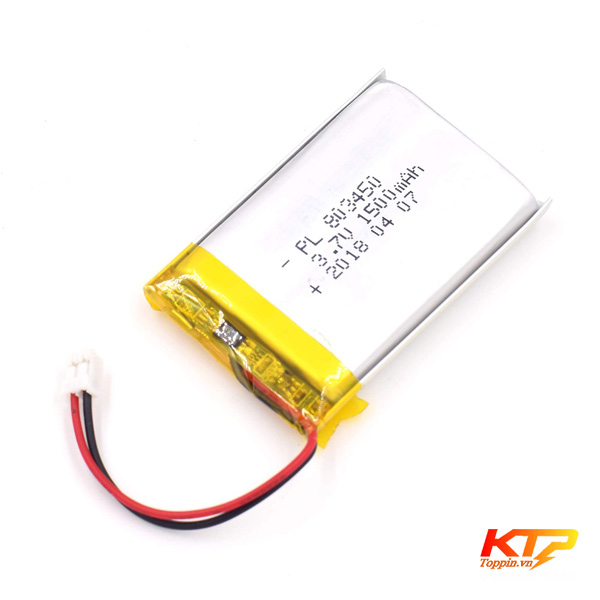
\includegraphics[width=0.5\textwidth]{Images/PinLithium.jpg}
        \captionsetup{font=small}  % Chỉnh kích thước chữ caption nhỏ
        \caption{Pin Lithium Polymer 3.7V 1500mAh (Model FL 803450).}
    \end{figure}
    
    
    Pin LiPo trong hệ thống MSMS được kết nối với module IP5306 thông qua đầu nối JST để quản lý quá trình sạc và xả. Khi có nguồn ngoài qua cổng USB Type-C của IP5306, pin sẽ được sạc với dòng điện tối đa 2.4A cho đến khi đạt điện áp 4.2V. Khi không có nguồn ngoài, pin sẽ cung cấp năng lượng cho hệ thống thông qua module IP5306, đảm bảo hệ thống có thể hoạt động liên tục trong thời gian dài mà không cần kết nối với nguồn điện lưới.

    Với dung lượng 1500mAh và điện áp danh định 3.7V, pin có thể cung cấp năng lượng cho hệ thống MSMS trong nhiều giờ tùy thuộc vào mức tiêu thụ công suất của các thành phần. Ở kịch bản Peak với hai cảm biến hoạt động đồng thời ở mức tiêu thụ cao nhất, pin có thể duy trì hoạt động khoảng 1.9 giờ. Trong điều kiện sử dụng thực tế với các chế độ tiết kiệm năng lượng, thời gian hoạt động có thể kéo dài từ 5.1 đến 6.9 giờ. Module IP5306 sẽ tự động quản lý chu kỳ sạc/xả và bảo vệ pin khỏi các tình huống nguy hiểm, kéo dài tuổi thọ và đảm bảo an toàn cho hệ thống.

    \item \phantomsection
    \addcontentsline{toc}{paragraph}{F) Module màn hình OLED SSD1306}
    \textbf{Module màn hình OLED SSD1306}

    SSD1306 là màn hình OLED (Organic Light Emitting Diode) với độ phân giải 128x64 pixel, sử dụng giao tiếp I2C hoặc SPI. Màn hình OLED có ưu điểm là tiêu thụ điện năng thấp, góc nhìn rộng, độ tương phản cao và có thể hiển thị trong điều kiện ánh sáng mạnh. SSD1306 rất phù hợp cho các ứng dụng IoT cần hiển thị thông tin trực quan với mức tiêu thụ năng lượng thấp.
    \begin{table}[H]
        \centering
        \caption{Thông số kỹ thuật SSD1306}
        \label{tab:ssd1306}
        \renewcommand{\arraystretch}{1.3}
        \begin{tabular}{|l|l|}
        \hline
        \textbf{Thông số} & \textbf{Giá trị} \\
        \hline
        Chức năng & Màn hình OLED hiển thị \\
        Kích thước & 0.96 inch \\
        Độ phân giải & 128 $\times$ 64 pixel \\
        Màu hiển thị & Trắng / Xanh \\
        Giao tiếp & I2C / SPI \\
        Điện áp hoạt động & 3.3 -- 5 V \\
        Dòng tiêu thụ & $\sim$20 mA \\
        \hline
        \end{tabular}
        \end{table}
    \begin{figure}[H]
        \centering
        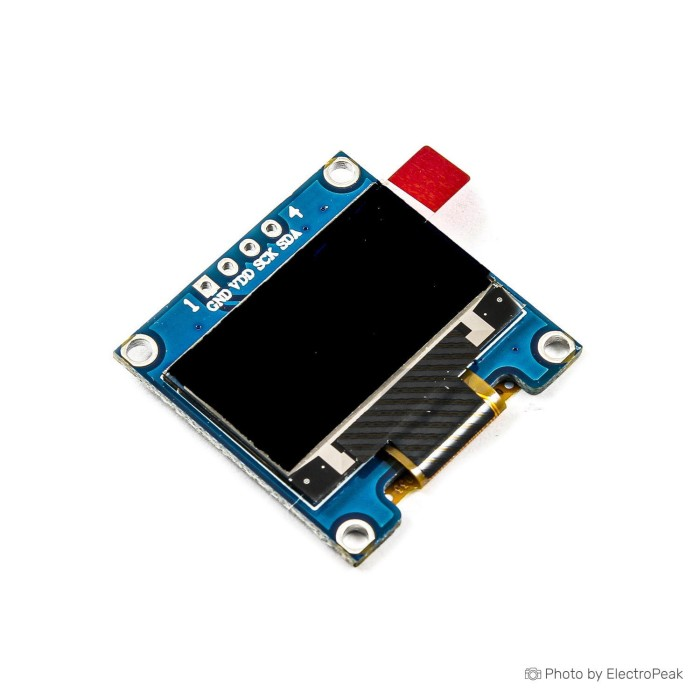
\includegraphics[width=0.3\textwidth]{Images/SSD1306.jpg}
        \captionsetup{font=small}
        \caption{Module màn hình OLED SSD1306.}
    \end{figure}


    Màn hình SSD1306 có thể hiển thị văn bản, số và đồ họa đơn giản, rất phù hợp để hiển thị các thông số quan trắc như PM2.5, PM10, nhiệt độ, độ ẩm và áp suất không khí. Màn hình có thể kết nối trực tiếp với ESP32 thông qua giao tiếp I2C, chỉ cần 2 chân (SDA, SCL), giúp tiết kiệm số chân GPIO và đơn giản hóa kết nối.

    \item \phantomsection
    \addcontentsline{toc}{paragraph}{G) IC ổn áp AMS1117-3.3}
    \textbf{IC ổn áp AMS1117-3.3}

    AMS1117-3.3 là IC ổn áp tuyến tính có khả năng cung cấp dòng điện lên đến 1A, được sử dụng để hạ điện áp từ nguồn pin xuống 3.3V để cấp nguồn cho ESP32 và các cảm biến. IC này có độ ổn định điện áp tốt, nhiễu thấp và giá thành rẻ, rất phù hợp cho các ứng dụng IoT tiêu thụ điện năng thấp.

    \begin{table}[H]
        \centering
        \caption{Thông số kỹ thuật AMS1117-3.3}
        \label{tab:ams1117}
        \renewcommand{\arraystretch}{1.3}
        \begin{tabular}{|l|l|}
        \hline
        \textbf{Thông số} & \textbf{Giá trị} \\
        \hline
        Chức năng & IC ổn áp tuyến tính \\
        Điện áp đầu vào & 4.5 -- 15 V \\
        Điện áp đầu ra & 3.3 V \\
        Dòng tối đa & 1 A \\
        Dropout Voltage & $\sim$1.1 V \\
        Kiểu đóng gói & SOT-223 \\
        Bảo vệ & Quá dòng, quá nhiệt \\
        \hline
        \end{tabular}
    \end{table}

    \begin{figure}[H]
        \centering
        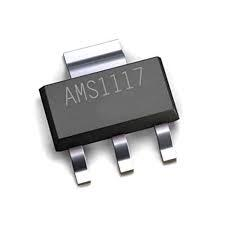
\includegraphics[width=0.4\textwidth]{Images/AMS1117.jpg}
        \captionsetup{font=small}
        \caption{IC ổn áp AMS1117-3.3.}
    \end{figure}

    AMS1117-3.3 hoạt động với điện áp đầu vào từ 4.75V đến 15V và cung cấp điện áp đầu ra ổn định 3.3V. IC này yêu cầu các tụ điện lọc đầu vào và đầu ra để đảm bảo hoạt động ổn định, thường là tụ 10µF ở đầu vào và tụ 22µF ở đầu ra. Trong hệ thống này, AMS1117-3.3 được sử dụng để hạ điện áp từ đầu ra 5V của module IP5306 xuống 3.3V để cấp nguồn cho ESP32 và các cảm biến hoạt động ở mức điện áp 3.3V.

    \item \phantomsection
    \addcontentsline{toc}{paragraph}{H) Màn hình TFT ILI9341}
    \textbf{Màn hình TFT ILI9341}

    ILI9341 là IC điều khiển màn hình màu tinh thể lỏng (TFT LCD) độ phân giải 240$\times$320 pixel, hỗ trợ hiển thị 262K màu. Trong dự án này, màn hình TFT được kết nối với mạch Gateway qua chuẩn giao tiếp SPI tốc độ cao để hiển thị trực quan dữ liệu thu thập được từ toàn bộ mạng Mesh. Với kích thước lớn và khả năng hiển thị đồ họa màu, TFT mang lại trải nghiệm quan sát tốt hơn so với màn hình OLED đơn sắc trên các node.
    
    \begin{table}[H]
        \centering
        \caption{Thông số kỹ thuật TFT ILI9341}
        \label{tab:ili9341}
        \renewcommand{\arraystretch}{1.3}
        \begin{tabular}{|l|l|}
        \hline
        \textbf{Thông số} & \textbf{Giá trị} \\
        \hline
        Độ phân giải & 240 $\times$ 320 pixel \\
        Màu sắc & 16-bit RGB (65K màu) / 18-bit (262K màu) \\
        Giao tiếp & SPI (4-wire) \\
        Điện áp hoạt động & 3.3 V \\
        IC điều khiển & ILI9341 \\
        Đèn nền & LED trắng (cần điều khiển độ sáng) \\
        \hline
        \end{tabular}
    \end{table}
    
    \begin{figure}[H]
        \centering
        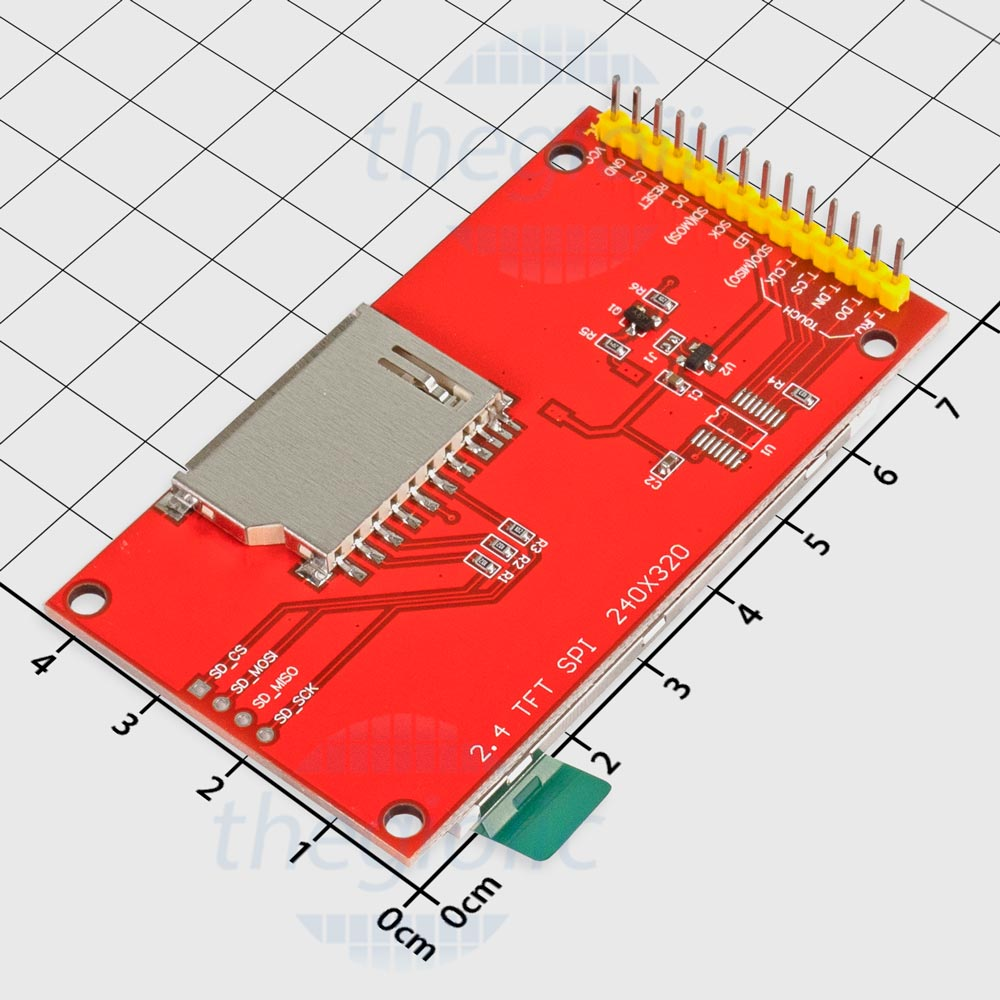
\includegraphics[width=0.4\textwidth]{Images/ili9341.jpg}
        \captionsetup{font=small}
        \caption{Màn hình TFT ILI9341.}
    \end{figure}

    \item \phantomsection
    \addcontentsline{toc}{paragraph}{I) IC mở rộng I/O PCF8574}
    \textbf{IC mở rộng I/O PCF8574}

    PCF8574 là IC mở rộng cổng vào/ra (I/O Expander) 8 bit giao tiếp qua bus I2C. IC này giúp vi điều khiển có thêm 8 chân GPIO hai chiều chỉ bằng cách sử dụng 2 chân I2C (SDA, SCL), qua đó giải quyết triệt để tình trạng thiếu hụt chân trên ESP32. Trong hệ thống, PCF8574 được dùng để đọc trạng thái các nút bấm và điều khiển các ngõ ra trạng thái khác mà không làm tốn chân GPIO của mạch chính.
    
    \begin{table}[H]
        \centering
        \caption{Thông số kỹ thuật PCF8574}
        \label{tab:pcf8574}
        \renewcommand{\arraystretch}{1.3}
        \begin{tabular}{|l|l|}
        \hline
        \textbf{Thông số} & \textbf{Giá trị} \\
        \hline
        Giao tiếp & I2C (tối đa 100 kHz) \\
        Số chân I/O & 8 bit (Quasi-bidirectional) \\
        Điện áp hoạt động & 2.5 V -- 6.0 V \\
        Dòng ngõ ra (Source) & Nhỏ (kéo dòng yếu) \\
        Dòng ngõ vào (Sink) & Lên đến 25 mA \\
        Ngắt (Interrupt) & Có ngõ ra INT \\
        \hline
        \end{tabular}
    \end{table}
    
    \begin{figure}[H]
        \centering
        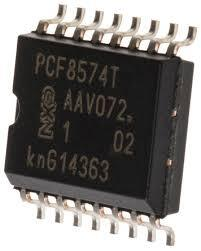
\includegraphics[width=0.4\textwidth]{Images/pcf8574.jpg}
        \captionsetup{font=small}
        \caption{IC mở rộng I/O PCF8574.}
    \end{figure}

    \item \phantomsection
    \addcontentsline{toc}{paragraph}{J) MOSFET AO3400 (N-Channel) và AO3401 (P-Channel)}
    \textbf{MOSFET AO3400 và AO3401}

    AO3400 và AO3401 là các MOSFET công suất thấp kiểu đóng gói SMD (SOT-23) được sử dụng rộng rãi trong các mạch điều khiển đóng ngắt (switching) và mạch quản lý nguồn (power path, reverse polarity protection).
    \begin{itemize}
        \item \textbf{AO3400 (N-Channel MOSFET):} Thường được dùng ở phía low-side (kéo xuống mass) để đóng/cắt nguồn cho các module cảm biến hoặc màn hình nhằm tiết kiệm pin khi vào chế độ ngủ (sleep mode). Mức $V_{GS(th)}$ thấp giúp nó có thể được kích dẫn hoàn toàn trực tiếp từ chân GPIO 3.3V của ESP32.
        \item \textbf{AO3401 (P-Channel MOSFET):} Thường được dùng ở phía high-side để đóng cắt nguồn dương hoặc tạo thành mạch chuyển đổi nguồn tự động (power path management), chống dòng ngược từ pin khi cắm sạc.
    \end{itemize}
    
    \begin{table}[H]
        \centering
        \caption{Thông số kỹ thuật MOSFET AO3400 và AO3401}
        \label{tab:mosfet_ao}
        \renewcommand{\arraystretch}{1.3}
        \begin{tabular}{|l|l|l|}
        \hline
        \textbf{Thông số} & \textbf{AO3400 (N-Channel)} & \textbf{AO3401 (P-Channel)} \\
        \hline
        Điện áp đánh thủng ($V_{DSS}$) & 30 V & -30 V \\
        Dòng xả liên tục ($I_D$) & 5.7 A & -4.2 A \\
        Điện trở bật ($R_{DS(ON)}$) @ 4.5V & $< 26.5 \text{ m}\Omega$ & $< 50 \text{ m}\Omega$ \\
        Điện áp ngưỡng ($V_{GS(th)}$) & 0.65 V -- 1.45 V & -0.65 V -- -1.3 V \\
        Kiểu đóng gói & SOT-23 & SOT-23 \\
        \hline
        \end{tabular}
    \end{table}
    
    \begin{figure}[H]
        \centering
        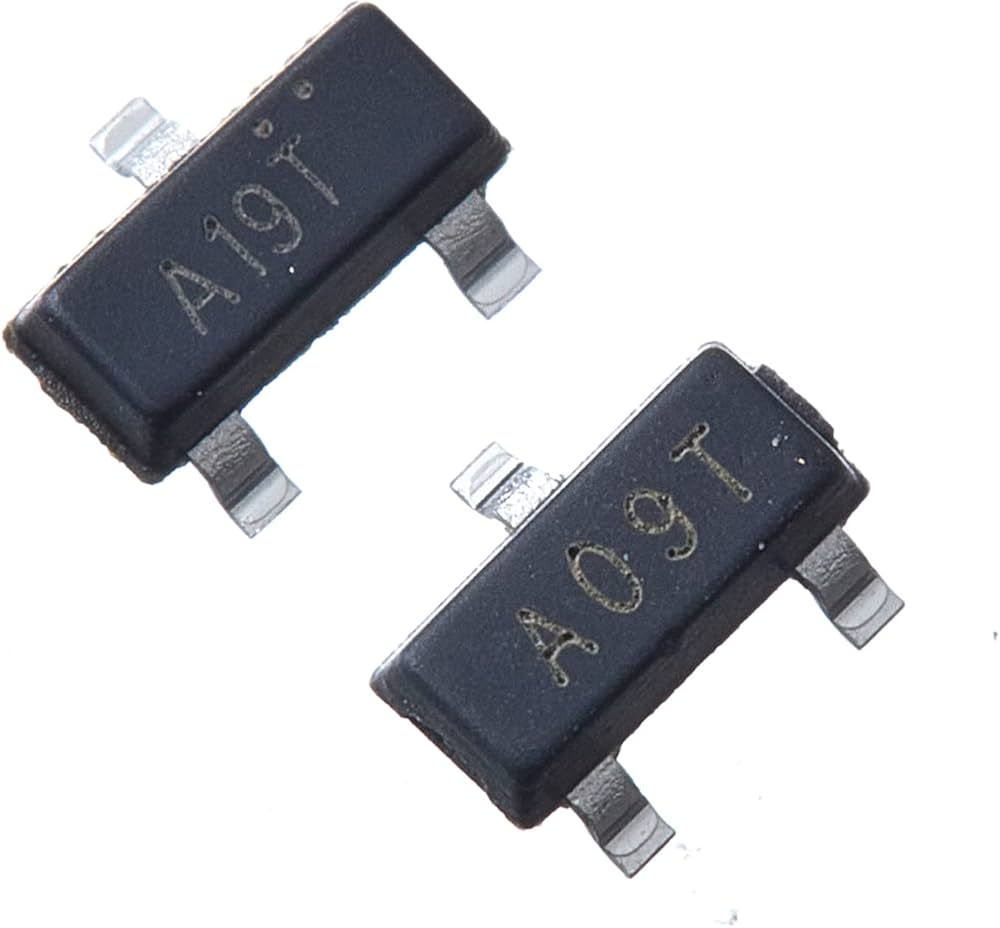
\includegraphics[width=0.4\textwidth]{Images/ao3400_1.jpg}
        \captionsetup{font=small}
        \caption{MOSFET AO3400 / AO3401 (Kiểu chân SOT-23).}
    \end{figure}

    \item \phantomsection
    \addcontentsline{toc}{paragraph}{K) IC giao tiếp USB-to-Serial CH340C}
    \textbf{IC giao tiếp USB-to-Serial CH340C}

    CH340C là một vi mạch chuyển đổi giao tiếp từ USB sang UART nối tiếp, thường được sử dụng trên các mạch nạp của ESP32. Đặc điểm nổi bật của CH340C là có sẵn bộ dao động thạch anh bên trong, giúp tiết kiệm không gian mạch và giảm chi phí linh kiện.
    
    \begin{table}[H]
        \centering
        \caption{Thông số kỹ thuật CH340C}
        \label{tab:ch340c}
        \renewcommand{\arraystretch}{1.3}
        \begin{tabular}{|l|l|}
        \hline
        \textbf{Thông số} & \textbf{Giá trị} \\
        \hline
        Giao tiếp & USB 2.0 to TTL UART \\
        Điện áp hoạt động & 3.3 V hoặc 5 V \\
        Tốc độ Baud & 50 bps -- 2 Mbps \\
        Dao động & Tích hợp sẵn (không cần thạch anh ngoài) \\
        Kiểu đóng gói & SOP-16 \\
        \hline
        \end{tabular}
    \end{table}

    \begin{figure}[H]
        \centering
        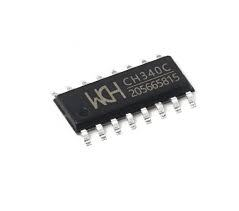
\includegraphics[width=0.4\textwidth]{Images/ch340c.jpg}
        \captionsetup{font=small}
        \caption{IC giao tiếp USB-to-Serial CH340C.}
    \end{figure}

    \item \phantomsection
    \addcontentsline{toc}{paragraph}{L) MOSFET BSS138 (Logic Level Shifter)}
    \textbf{MOSFET BSS138}

    BSS138 là một N-Channel MOSFET công suất thấp, thường được sử dụng trong các mạch chuyển đổi mức điện áp logic (Logic Level Converter) hai chiều. Vi điều khiển ESP32 hoạt động ở mức logic 3.3V, trong khi một số cảm biến hoặc module phụ trợ lại yêu cầu mức logic 5V. BSS138 đóng vai trò cầu nối an toàn, đảm bảo tín hiệu giao tiếp (như I2C, UART) truyền đi thông suốt giữa 2 mức điện áp mà không làm hỏng chân vi điều khiển.
    
    \begin{table}[H]
        \centering
        \caption{Thông số kỹ thuật MOSFET BSS138}
        \label{tab:bss138}
        \renewcommand{\arraystretch}{1.3}
        \begin{tabular}{|l|l|}
        \hline
        \textbf{Thông số} & \textbf{Giá trị} \\
        \hline
        Loại & N-Channel MOSFET \\
        Điện áp đánh thủng ($V_{DSS}$) & 50 V \\
        Dòng xả liên tục ($I_D$) & 220 mA \\
        Điện trở bật ($R_{DS(ON)}$) & $< 3.5 \text{ } \Omega$ \\
        Điện áp ngưỡng ($V_{GS(th)}$) & 0.8 V -- 1.5 V (Rất nhạy) \\
        Kiểu đóng gói & SOT-23 \\
        \hline
        \end{tabular}
    \end{table}

    \begin{figure}[H]
        \centering
        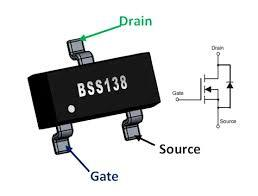
\includegraphics[width=0.4\textwidth]{Images/bss138.jpg}
        \captionsetup{font=small}
        \caption{MOSFET BSS138 (SOT-23).}
    \end{figure}

\end{enumerate}



\subsection{Thiết kế chi tiết hệ thống}
Trong dự án này, phần cứng được chia làm 2 thành phần mạch độc lập: \textbf{Mạch MSMS Node} và \textbf{Mạch Gateway}. 

\subsubsection{Thiết kế phần cứng mạch MSMS Node}
Mạch MSMS Node có chức năng thu thập dữ liệu cảm biến, hiển thị cục bộ và truyền tải lên mạng Mesh. Mạch tích hợp nhiều linh kiện quan trọng như thẻ nhớ SD Card, RTC DS3231, IC nạp CH340C và các khối đóng ngắt nguồn bằng MOSFET (AO3400, AO3401).

\paragraph{A. Tính toán đáp ứng công suất nguồn} \mbox{}\\
Hệ thống được cấp nguồn từ pin lithium thông qua module quản lý nguồn IP5306. Module IP5306 có khả năng sạc pin và cung cấp đầu ra 5V ổn định cho hệ thống. Điện áp 5V từ IP5306 được hạ xuống 3.3V thông qua IC ổn áp tuyến tính AMS1117-3.3 để cấp nguồn cho ESP32 và các cảm biến hoạt động ở mức điện áp 3.3V.

AMS1117-3.3 là IC ổn áp tuyến tính có khả năng cung cấp dòng điện lên đến 1A, phù hợp cho các ứng dụng IoT tiêu thụ điện năng thấp. IC này có độ ổn định điện áp tốt và nhiễu thấp, đảm bảo nguồn cung cấp ổn định cho hệ thống. Để đảm bảo hoạt động ổn định, cần sử dụng các tụ điện lọc đầu vào và đầu ra phù hợp (thường là 10µF và 22µF).


\textbf{Phân tích công suất:}
\begin{table}[H]
    \centering
    \caption{Bảng tính toán công suất nguồn Node MSMS ở kịch bản Peak}
    \label{tab:power_peak_msms}
    \renewcommand{\arraystretch}{1.3}
    \makebox[\textwidth][c]{%
    \begin{tabular}{|l|c|c|c|}
    \hline
    \textbf{Linh kiện} & \textbf{Điện áp (V)} & \textbf{Dòng Peak (mA)} & \textbf{Công suất (W)} \\
    \hline
    ESP32 & 3.3 & 240 & 0.792 \\
    SSD1306 OLED & 3.3 & 30 & 0.099 \\
    DS3231 & 3.3 & 0.2 & 0.001 \\
    Thẻ SD (SPI) & 3.3 & 100 & 0.330 \\
    3 cảm biến & 3.3 & 45 & 0.149 \\
    CH340C & 3.3 & 15 & 0.050 \\
    \hline
    \textbf{Tổng tải 3.3V} & -- & \textbf{430.2} & \textbf{1.421} \\
    \hline
    \textbf{Tổn hao AMS1117} & 5 $\rightarrow$ 3.3 & -- & \textbf{0.731} \\
    \hline
    \textbf{TỔNG CÔNG SUẤT NGUỒN 5V} & \textbf{5} & \textbf{430.2} & \textbf{2.152} \\
    \hline
    \end{tabular}%
    }
\end{table}
    
Từ bảng tính toán trên, do sử dụng IC ổn áp tuyến tính AMS1117, dòng điện tiêu thụ ở mức 5V bằng dòng tiêu thụ ở 3.3V. Tổng công suất tải ở 5V là 2.152 W (tương ứng dòng 430.2 mA). Tính toán lượng điện năng rút từ pin Lithium qua module IP5306 (hiệu suất boost khoảng 92.5\%):
\[
P_{in} = \frac{2.152}{0.925} \approx 2.326 \text{ W}
\]
Với điện áp pin trung bình khoảng 3.7V, dòng điện đầu vào từ pin:
\[
I_{in} = \frac{2.326}{3.7} \approx 629 \text{ mA}
\]

Với pin lithium dung lượng 1500mAh, thời gian hoạt động lý thuyết ở kịch bản Peak (tất cả module cùng chạy ở công suất tối đa):
\[
T_{peak} = \frac{1500}{629} \approx 2.38 \text{ giờ}
\]

Trong thực tế, nhờ các chế độ tiết kiệm năng lượng (như đóng MOSFET AO3400 ngắt các cảm biến, đưa ESP32 vào deep sleep, tắt OLED, SD Card ở idle), công suất tiêu thụ trung bình được giảm đáng kể. Dòng xả thực tế chỉ ở mức 150 - 250 mA, giúp hệ thống kéo dài thời gian hoạt động lên đến 6 - 10 giờ. Module IP5306 cũng có tính năng tự động tắt đầu ra khi tải thấp (<50mA), tuy nhiên thiết kế đã đảm bảo dòng sleep của hệ thống không tụt quá sâu để tránh mất nguồn đột ngột.





\paragraph{B. Thiết kế mạch nguyên lý (Schematic)} \mbox{}\\

\begin{figure}[H]
    \centering
    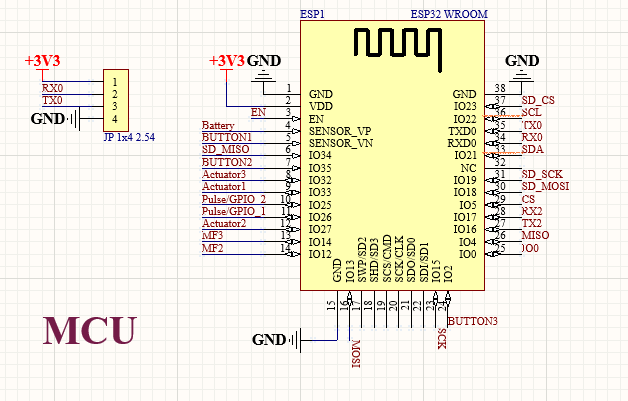
\includegraphics[width=0.8\textwidth]{Images/KhoiMCU.png}
    \captionsetup{font=small}
    \caption{Khối xử lý và nút bấm.}
\end{figure}
Khối MCU là trung tâm điều khiển của hệ thống, bao gồm:

\begin{itemize}
    \item \textbf{Module ESP32 WROOM:} Vi điều khiển chính đảm nhận việc xử lý dữ liệu, giao tiếp mạng Mesh/Wi-Fi và điều khiển các ngoại vi.
    \item \textbf{Header nạp chương trình (JP 1x4):} Cung cấp các chân giao tiếp UART cơ bản (RX0, TX0) cùng nguồn cấp (+3V3, GND) để kết nối với mạch nạp USB-to-Serial rời (như CH340C) khi cần nạp firmware hoặc debug. Thiết kế này giúp tối giản linh kiện trên bo mạch chính.
\end{itemize}

\begin{figure}[H]
    \centering
    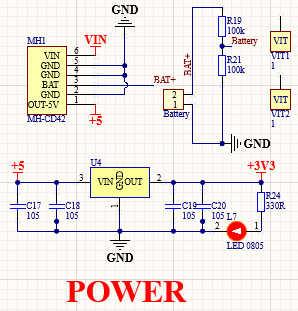
\includegraphics[width=0.9\textwidth]{Images/KhoiNguon.png}
    \captionsetup{font=small}
    \caption{Khối nguồn.}
\end{figure}

Khối nguồn sử dụng module tích hợp MH-CD42 (dựa trên lõi IP5306) để quản lý nguồn pin và cung cấp điện áp hoạt động cho hệ thống:

\begin{itemize}
    \item \textbf{Đầu vào pin lithium:} Header 2 chân (Header 2P 2.54) kết nối với pin lithium (VCC\_BAT và GND\_BAT).
    
    \item \textbf{Module quản lý nguồn MH-CD42 (ICBUCK1):} Đây là mạch tích hợp hoàn chỉnh dựa trên IC IP5306, cung cấp các chức năng ưu việt:
    \begin{itemize}
        \item \textbf{Sạc và Boost áp:} Quản lý sạc pin qua cổng USB và tự động kích áp (boost converter) từ điện áp pin lên mức 5V ổn định (VCC\_OUT).
        \item \textbf{Chuyển mạch nguồn tự động (Power Path):} Mạch MH-CD42 đã được tích hợp sẵn tính năng Power Path phần cứng bên trong. Khi cắm sạc, hệ thống sẽ tự động sử dụng trực tiếp nguồn ngoài để nuôi tải và đồng thời sạc pin, ngắt hoàn toàn đường xả của pin. Điều này giúp hệ thống không bị tình trạng vừa sạc vừa xả (tránh chai pin) và đảm bảo IC nhận diện đúng mức sạc đầy.
        \item \textbf{Hiển thị mức pin:} Tích hợp sẵn hệ thống 4 LED báo dung lượng, giúp theo dõi trực quan mức pin còn lại của Node.
    \end{itemize}
    
    \item \textbf{Mạch giám sát pin phụ (Cap\_Battery):} Dù MH-CD42 có hiển thị LED, mạch vẫn thiết kế thêm bộ chia áp bằng hai điện trở 100k$\Omega$ (R20, R21). Mạch này đưa điện áp pin về ngưỡng 0-3.3V an toàn cho ADC của ESP32, giúp vi điều khiển chủ động đo lường và gửi phần trăm pin lên hệ thống theo thời gian thực.
    
    \item \textbf{IC ổn áp AMS1117-3.3 (U2):} Hạ điện áp từ 5V xuống 3.3V để cấp nguồn nuôi ESP32 và các IC logic. Có các tụ lọc đầu vào (C2, C3) và đầu ra (C5, C6) để đảm bảo nguồn cấp phẳng và chống nhiễu.
    
    \item \textbf{LED báo và Công tắc nguồn:} Trang bị công tắc gạt (S1) để bật/tắt điện áp 3.3V cho hệ thống, kèm theo LED báo trạng thái cấp nguồn.
\end{itemize}

\begin{figure}[H]
    \centering
    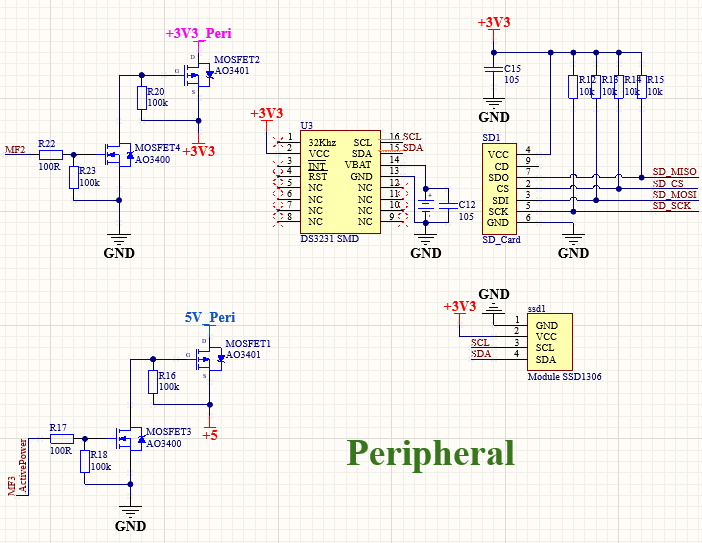
\includegraphics[width=0.9\textwidth]{Images/KhoiPeripheral.png}
    \captionsetup{font=small}
    \caption{Khối ngoại vi (Peripheral).}
\end{figure}
Khối Peripheral bao gồm các module cố định trên bo mạch và mạch đóng ngắt nguồn cho các ngoại vi:

\begin{itemize}
    \item \textbf{Mạch chuyển mạch nguồn (High-side Load Switch):} Sử dụng kết hợp N-Channel MOSFET (AO3400) để kích chân Gate của P-Channel MOSFET (AO3401). Có hai mạch đóng ngắt riêng biệt cho nhánh nguồn \textbf{+3V3\_Peri} (điều khiển bởi chân MF2) và nhánh \textbf{5V\_Peri} (điều khiển bởi chân MF3\_ActivePower). Thiết kế này cho phép ESP32 ngắt hoàn toàn nguồn điện cấp cho các cảm biến và ngoại vi bên ngoài khi chuyển sang chế độ Deep Sleep, giúp tối ưu hóa công suất tiêu thụ của Node.
    
    \item \textbf{Module RTC DS3231 (U3):} IC đồng hồ thời gian thực giao tiếp qua I2C (SCL, SDA), được cấp nguồn trực tiếp từ +3V3 để luôn duy trì đếm thời gian. Tích hợp đế pin dự phòng để giữ giờ khi mất nguồn chính.
    
    \item \textbf{Module thẻ nhớ Micro SD (SD1):} Kết nối qua giao tiếp SPI (MISO, MOSI, SCK, CS), được kéo lên (pull-up) bằng các điện trở 10k$\Omega$ trên các đường tín hiệu để đảm bảo truyền nhận dữ liệu ổn định với thẻ nhớ.
    
    \item \textbf{Màn hình OLED SSD1306 (ssd1):} Giao tiếp qua bus I2C chung với RTC, dùng để hiển thị các thông số trạng thái tại Node.
\end{itemize}

\begin{figure}[H]
    \centering
    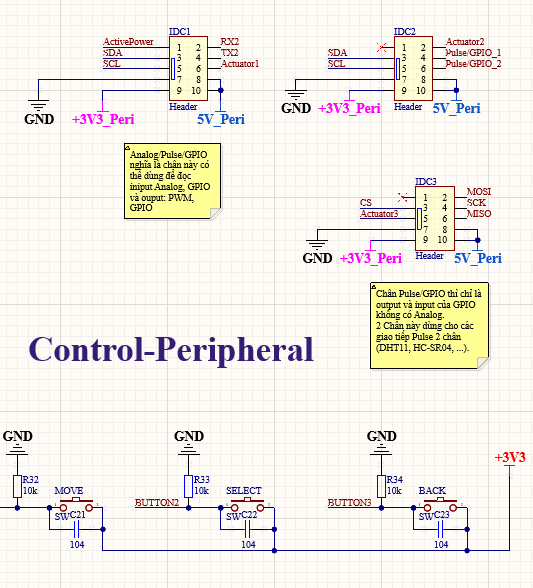
\includegraphics[width=0.9\textwidth]{Images/KhoiControlPeripheral.png}
    \captionsetup{font=small}
    \caption{Khối điều khiển và kết nối ngoại vi mở rộng (Control-Peripheral).}
\end{figure}
Khối này thiết kế các cổng kết nối cảm biến độc lập (IDC) cùng hệ thống nút bấm điều khiển cục bộ:

\begin{itemize}
    \item \textbf{Các cổng kết nối (IDC1, IDC2, IDC3):} Được thiết kế theo chuẩn Header, cung cấp đồng thời 2 mức nguồn có thể đóng ngắt (\textbf{+3V3\_Peri} và \textbf{5V\_Peri}) cùng nhiều chuẩn giao tiếp:
    \begin{itemize}
        \item \textbf{IDC1:} Cung cấp bus I2C (SDA, SCL), UART (RX2, TX2) và chân điều khiển Actuator1. 
        \item \textbf{IDC2:} Chuyên dụng cho các tín hiệu số, tích hợp Actuator2 và 2 chân Pulse/GPIO (dùng cho cảm biến DHT11, HC-SR04...). Không có ngõ vào Analog.
        \item \textbf{IDC3:} Cung cấp bus SPI (MOSI, MISO, SCK, CS) cho các module giao tiếp tốc độ cao và Actuator3.
    \end{itemize}
    \item \textbf{Hệ thống nút bấm điều khiển:} Bao gồm 3 nút nhấn (MOVE, SELECT, BACK). Mạch nút nhấn được thiết kế theo cấu hình kéo xuống (Pull-down) với điện trở 10k$\Omega$ nối GND, khi nhấn sẽ tạo tín hiệu mức CAO (+3V3). Mỗi nút đều được gắn song song với một tụ điện 104 (0.1µF) để chống dội phím phần cứng (hardware debounce), đảm bảo tín hiệu cấp vào ESP32 luôn ổn định. Chân tín hiệu của nút BACK (BUTTON3) được nối trực tiếp vào chân IO0 của ESP32, cho phép tận dụng nút này để đưa mạch vào chế độ bootloader khi cấp nguồn.
\end{itemize}
\subsubsection{Layout PCB}
\begin{figure}[H]
    \centering
    \begin{minipage}{0.48\textwidth}
        \centering
        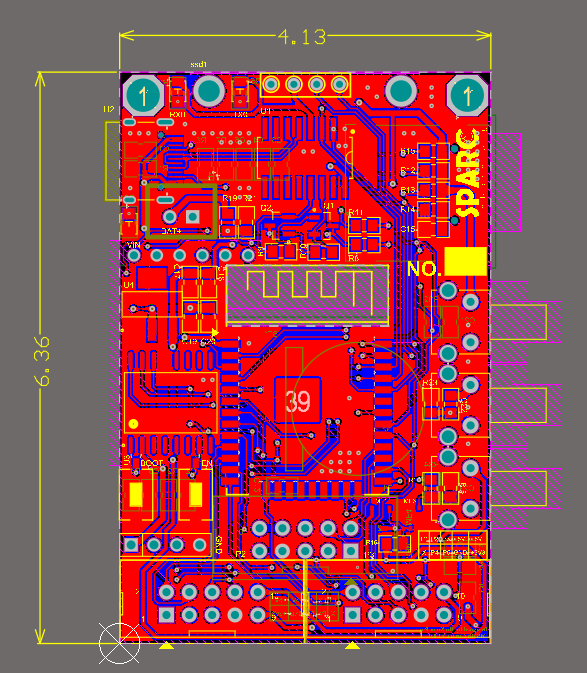
\includegraphics[width=\textwidth]{Images/TopLayer.png}
        \captionsetup{font=small}
        \caption{Lớp Top (Đường tín hiệu).}
        \label{toplayer}
    \end{minipage}\hfill
    \begin{minipage}{0.48\textwidth}
        \centering
        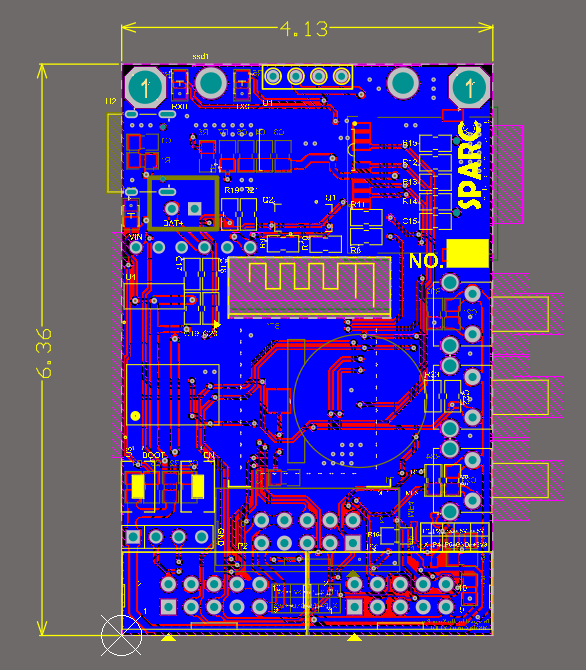
\includegraphics[width=\textwidth]{Images/BotLayer.png}
        \captionsetup{font=small}
        \caption{Lớp Bottom (Mặt dưới).}
        \label{botlayer}
    \end{minipage}
\end{figure}

\begin{figure}[H]
    \centering
    \begin{minipage}{0.48\textwidth}
        \centering
        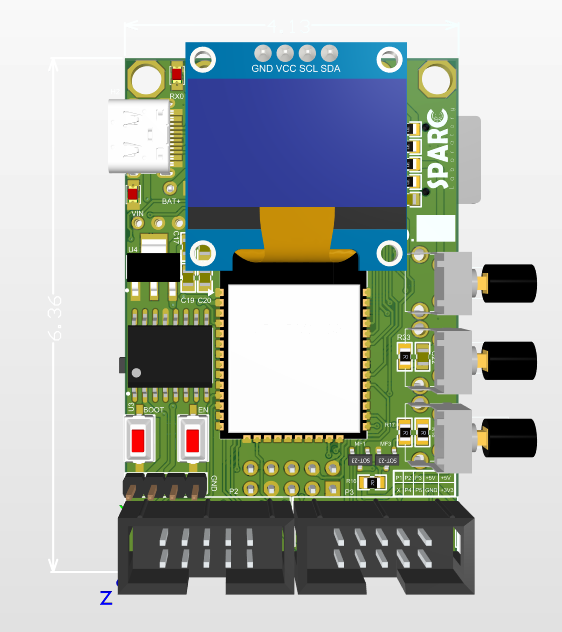
\includegraphics[width=\textwidth]{Images/3DTopLayer.png}
        \captionsetup{font=small}
        \caption{Mô hình 3D (Mặt trên).}
    \end{minipage}\hfill
    \begin{minipage}{0.48\textwidth}
        \centering
        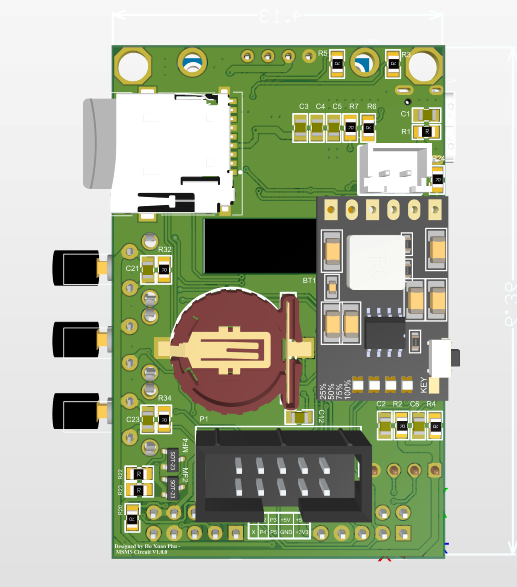
\includegraphics[width=\textwidth]{Images/3DBotLayer.png}
        \captionsetup{font=small}
        \caption{Mô hình 3D (Mặt dưới).}
    \end{minipage}
\end{figure}

\subsubsection{Thiết kế phần cứng mạch Gateway}
Mạch Gateway tập trung vào khả năng xử lý tốc độ cao, gom dữ liệu tập trung và kết nối mạng diện rộng. Khác với MSMS Node chạy bằng pin, Gateway thường hoạt động với nguồn cắm liên tục do cần hiệu suất CPU lớn để phân tích JSON và mã hoá kết nối mạng. Gateway giao tiếp với mạch MSMS Root qua UART tốc độ $\ge$ 921,600 bps. Ngoài việc đẩy dữ liệu lên đám mây, mạch Gateway còn tích hợp màn hình TFT ILI9341 (qua SPI) để trực quan hoá biểu đồ và lưu trữ log định kỳ vào thẻ nhớ SD Card (qua SPI). 

\paragraph{A. Tính toán đáp ứng công suất nguồn Gateway} \mbox{}\\
Vì Gateway có tính chất hoạt động 24/7 và chạy các ngoại vi công suất cao (như màn hình TFT), mạch cần một nguồn nuôi adapter 5V thay vì pin. Nguồn 5V này sẽ được hạ áp xuống 3.3V thông qua IC tuyến tính AMS1117-3.3.

\textbf{Phân tích công suất tải mạch Gateway:}
\begin{table}[H]
    \centering
    \caption{Bảng tính toán công suất nguồn định mức mạch Gateway}
    \label{tab:power_peak_gateway}
    \renewcommand{\arraystretch}{1.3}
    \makebox[\textwidth][c]{%
    \begin{tabular}{|l|c|c|c|}
    \hline
    \textbf{Linh kiện} & \textbf{Điện áp (V)} & \textbf{Dòng Peak (mA)} & \textbf{Công suất (W)} \\
    \hline
    ESP32 & 3.3 & 240 & 0.792 \\
    Màn hình TFT ILI9341 & 3.3 & 100 & 0.330 \\
    DS3231 & 3.3 & 0.2 & 0.001 \\
    Thẻ SD (SPI) & 3.3 & 100 & 0.330 \\
    IC mở rộng I/O PCF8574 & 3.3 & 1 & 0.003 \\
    CH340C & 3.3 & 15 & 0.050 \\
    \hline
    \textbf{Tổng tải 3.3V} & -- & \textbf{456.2} & \textbf{1.506} \\
    \hline
    \textbf{Tổn hao AMS1117} & 5 $\rightarrow$ 3.3 & -- & \textbf{0.775} \\
    \hline
    \textbf{TỔNG CÔNG SUẤT NGUỒN 5V} & \textbf{5} & \textbf{456.2} & \textbf{2.281} \\
    \hline
    \end{tabular}%
    }
\end{table}

Từ bảng tính toán trên, dòng điện tổng tiêu thụ tại nhánh 5V của mạch Gateway là khoảng 456.2 mA (với công suất 2.281 W). Do đó, mạch Gateway yêu cầu một adapter 5V với dòng cấp tối thiểu 1A (5W) để đảm bảo không bị sụt áp khi ESP32 truyền phát Wi-Fi liên tục và màn hình TFT bật sáng tối đa.

\paragraph{B. Thiết kế mạch nguyên lý (Schematic) Gateway} \mbox{}\\

\begin{figure}[H]
    \centering
    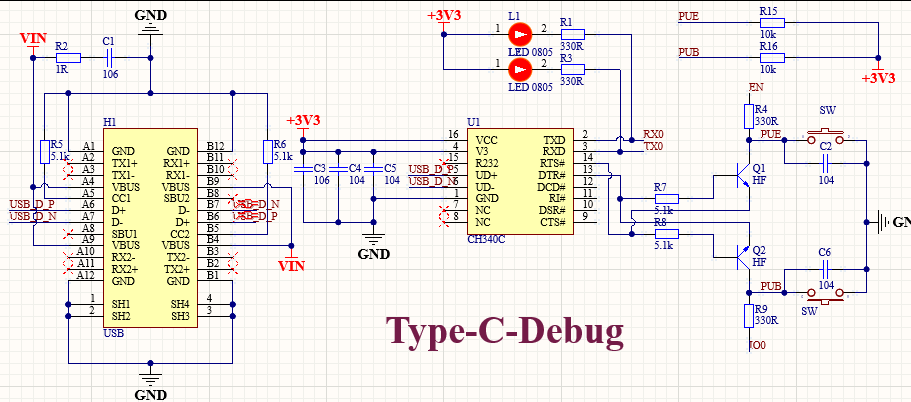
\includegraphics[width=0.8\textwidth]{Images/KhoiTypeC_Debug-gateway.png}
    \captionsetup{font=small}
    \caption{Khối mạch nạp và giao tiếp USB (Type-C-Debug) của Gateway.}
\end{figure}
Khối Type-C-Debug cung cấp giao tiếp USB cho Gateway với các chức năng:
\begin{itemize}
    \item \textbf{Cổng USB Type-C (H1):} Nhận điện áp cấp (VIN) cho hệ thống và truyền nhận tín hiệu dữ liệu USB (USB\_D\_P, USB\_D\_N).
    \item \textbf{IC chuyển đổi USB-to-UART (CH340C):} Tích hợp trực tiếp trên mạch, chuyển đổi tín hiệu USB sang giao tiếp UART (RX0, TX0) để nạp chương trình và debug với ESP32. Có tích hợp sẵn 2 LED báo trạng thái truyền/nhận dữ liệu.
    \item \textbf{Mạch Auto-Program:} Sử dụng 2 transistor S8050 (Q1, Q2) kết nối với các chân DTR và RTS của CH340C để tự động điều khiển các chân EN và IO0 của ESP32, giúp nạp code tự động mà không cần phải can thiệp ấn nút vật lý.
    \item \textbf{Nút bấm Boot/Reset:} Bố trí sẵn hai nút bấm vật lý kết nối vào đường PUE (EN) và PUB (IO0) để thao tác thủ công khi cần thiết.
\end{itemize}

\begin{figure}[H]
    \centering
    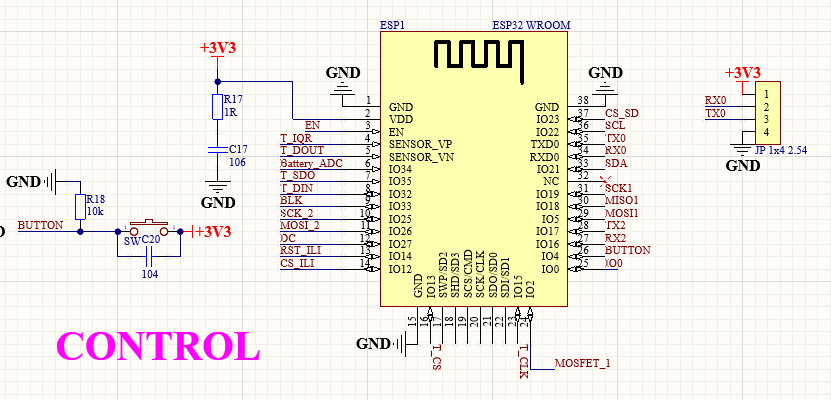
\includegraphics[width=0.9\textwidth]{Images/KhoiControl-GateWay.png}
    \captionsetup{font=small}
    \caption{Khối MCU điều khiển trung tâm của Gateway.}
\end{figure}
Khối MCU của Gateway được thiết kế xoay quanh ESP32:
\begin{itemize}
    \item \textbf{Module ESP32 WROOM:} Đảm nhận nhiệm vụ kết nối mạng Mesh/Wi-Fi, xử lý luồng dữ liệu lớn và điều khiển toàn bộ thiết bị ngoại vi của Gateway.
    \item \textbf{Mạch lọc chống nhiễu khởi động:} Chân EN được gắn mạch RC (điện trở R17 1$\Omega$, tụ C17 10µF) giúp ổn định tín hiệu điện áp khi mạch vừa được cấp nguồn.
    \item \textbf{Nút điều khiển ngoại vi:} Một nút nhấn đa dụng (BUTTON) kết nối vào chân IO4, sử dụng cấu hình Active-High (kéo xuống GND bằng điện trở 10k$\Omega$) kết hợp tụ 104 dội phím phần cứng.
\end{itemize}

\begin{figure}[H]
    \centering
    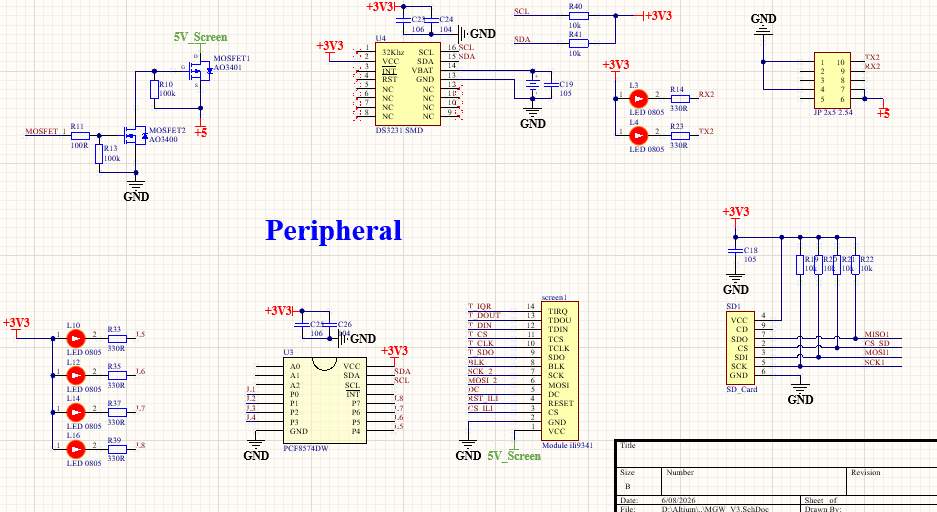
\includegraphics[width=0.9\textwidth]{Images/KhoiPeripheral-GateWay.png}
    \captionsetup{font=small}
    \caption{Khối ngoại vi (Peripheral) của Gateway.}
\end{figure}
Khối Peripheral của Gateway rất đa dạng do mạch đảm nhận vai trò hiển thị và trung chuyển dữ liệu trung tâm:
\begin{itemize}
    \item \textbf{Màn hình TFT ILI9341:} Màn hình màu hiển thị đồ thị và số liệu. Sử dụng giao tiếp SPI cho phần hiển thị và giao tiếp SPI rời cho mạch điều khiển cảm ứng. Đặc biệt, đường nguồn \textbf{5V\_Screen} cấp cho màn hình được thiết kế chạy qua mạch \textbf{High-Side Load Switch} (sử dụng N-MOSFET AO3400 kích P-MOSFET AO3401). Điều này cho phép vi điều khiển tắt hoàn toàn màn hình để tiết kiệm điện và chống nóng khi hệ thống chỉ cần chạy ngầm.
    \item \textbf{Module Thẻ nhớ SD (SD\_Card):} Kết nối qua bus SPI độc lập (MOSI1, MISO1, SCK1, CS\_SD) với các điện trở kéo lên 10k$\Omega$. Chức năng chính là lưu trữ (ghi log) toàn bộ dữ liệu thu thập từ mạng Mesh xuống thẻ nhớ định kỳ.
    \item \textbf{RTC DS3231:} Đồng hồ thời gian thực giao tiếp qua I2C, duy trì và cung cấp nhãn thời gian (timestamp) chính xác tuyệt đối để lưu file CSV vào thẻ nhớ.
    \item \textbf{IC mở rộng I/O PCF8574DW:} Do số lượng ngoại vi quá lớn làm cạn kiệt chân GPIO của ESP32, mạch sử dụng IC mở rộng I/O qua chuẩn I2C. Bốn chân đầu ra của PCF8574 được dùng để điều khiển dàn 4 LED báo trạng thái trực quan.
    \item \textbf{Giao tiếp UART MSMS Root:} Giao tiếp UART tốc độ cao (TX2, RX2) dùng để truyền nhận dữ liệu với mạch MSMS Root được nối ra header cắm. Các đường truyền này cũng được trích xuất qua cụm LED báo để theo dõi trực quan luồng traffic.
\end{itemize}

\paragraph{C. Layout PCB mạch Gateway} \mbox{}\\
Thiết kế PCB của Gateway được bố trí mật độ cao nhằm nhồi nhét nhiều linh kiện, nhưng đồng thời vẫn đảm bảo chất lượng truyền dẫn cho các đường tín hiệu tốc độ cao như SPI màn hình và UART luồng dữ liệu Mesh. 

\begin{figure}[H]
    \centering
    \begin{minipage}{0.48\textwidth}
        \centering
        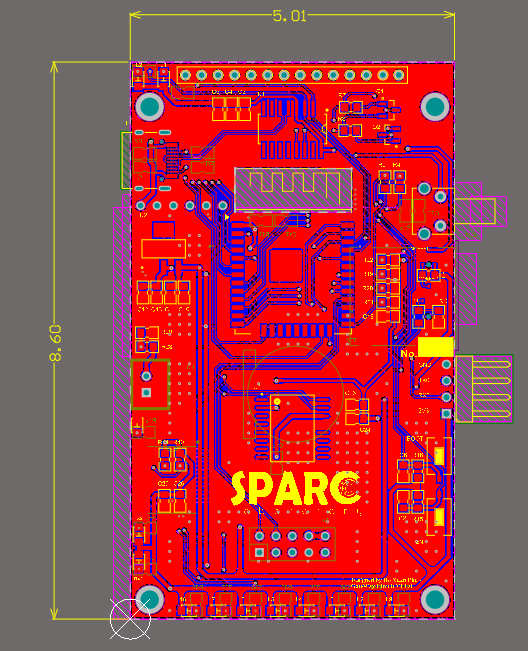
\includegraphics[width=\textwidth]{Images/TopLayer-GateWay.png}
        \captionsetup{font=small}
        \caption{Lớp Top (Đường tín hiệu).}
    \end{minipage}\hfill
    \begin{minipage}{0.48\textwidth}
        \centering
        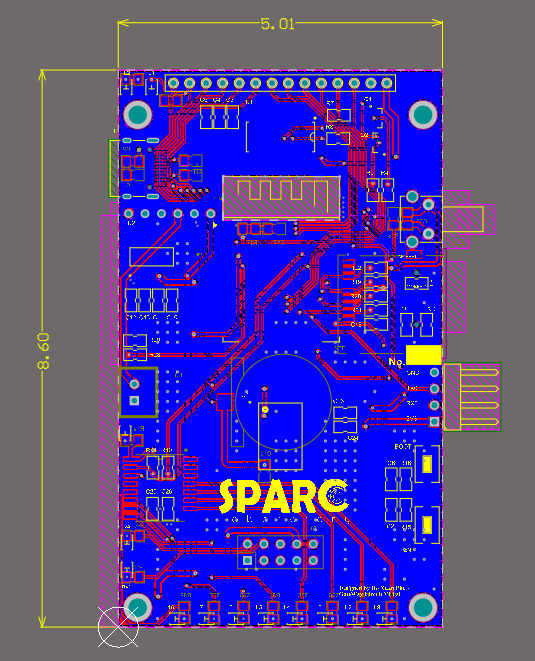
\includegraphics[width=\textwidth]{Images/BotLayer-Gateway.png}
        \captionsetup{font=small}
        \caption{Lớp Bottom (Mặt dưới).}
    \end{minipage}
\end{figure}

\begin{figure}[H]
    \centering
    \begin{minipage}{0.48\textwidth}
        \centering
        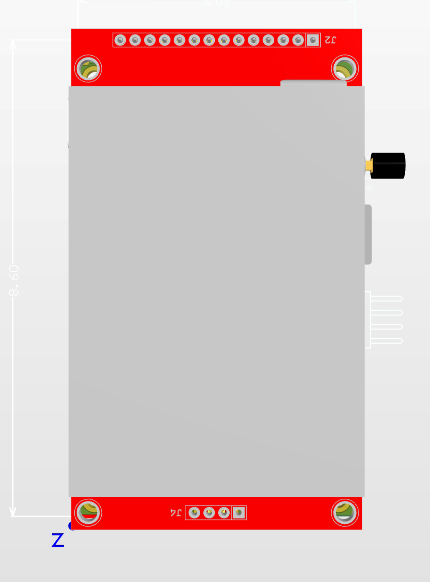
\includegraphics[width=\textwidth]{Images/3DTopLayer-Gateway.png}
        \captionsetup{font=small}
        \caption{Mô hình 3D (Mặt trên).}
    \end{minipage}\hfill
    \begin{minipage}{0.48\textwidth}
        \centering
        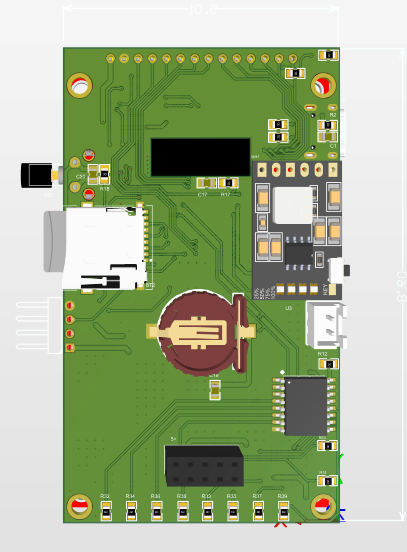
\includegraphics[width=\textwidth]{Images/3DBotLayer-gateway.png}
        \captionsetup{font=small}
        \caption{Mô hình 3D (Mặt dưới).}
    \end{minipage}
\end{figure}

\subsubsection{Thiết kế Firmware}

\paragraph{A. Thiết kế Firmware MSMS} \mbox{}\\

Trong dự án này, ESP32 được sử dụng làm bộ xử lý trung tâm của hệ thống, đảm nhận việc đọc dữ liệu từ các cảm biến và truyền tải lên mạng Mesh. Firmware của ESP32 được thiết kế theo kiến trúc phân lớp (layered architecture) với sự phân tách rõ ràng giữa các tầng ứng dụng, hệ điều hành, thư viện, driver và phần cứng vật lý.

\begin{figure}[H]
    \centering
    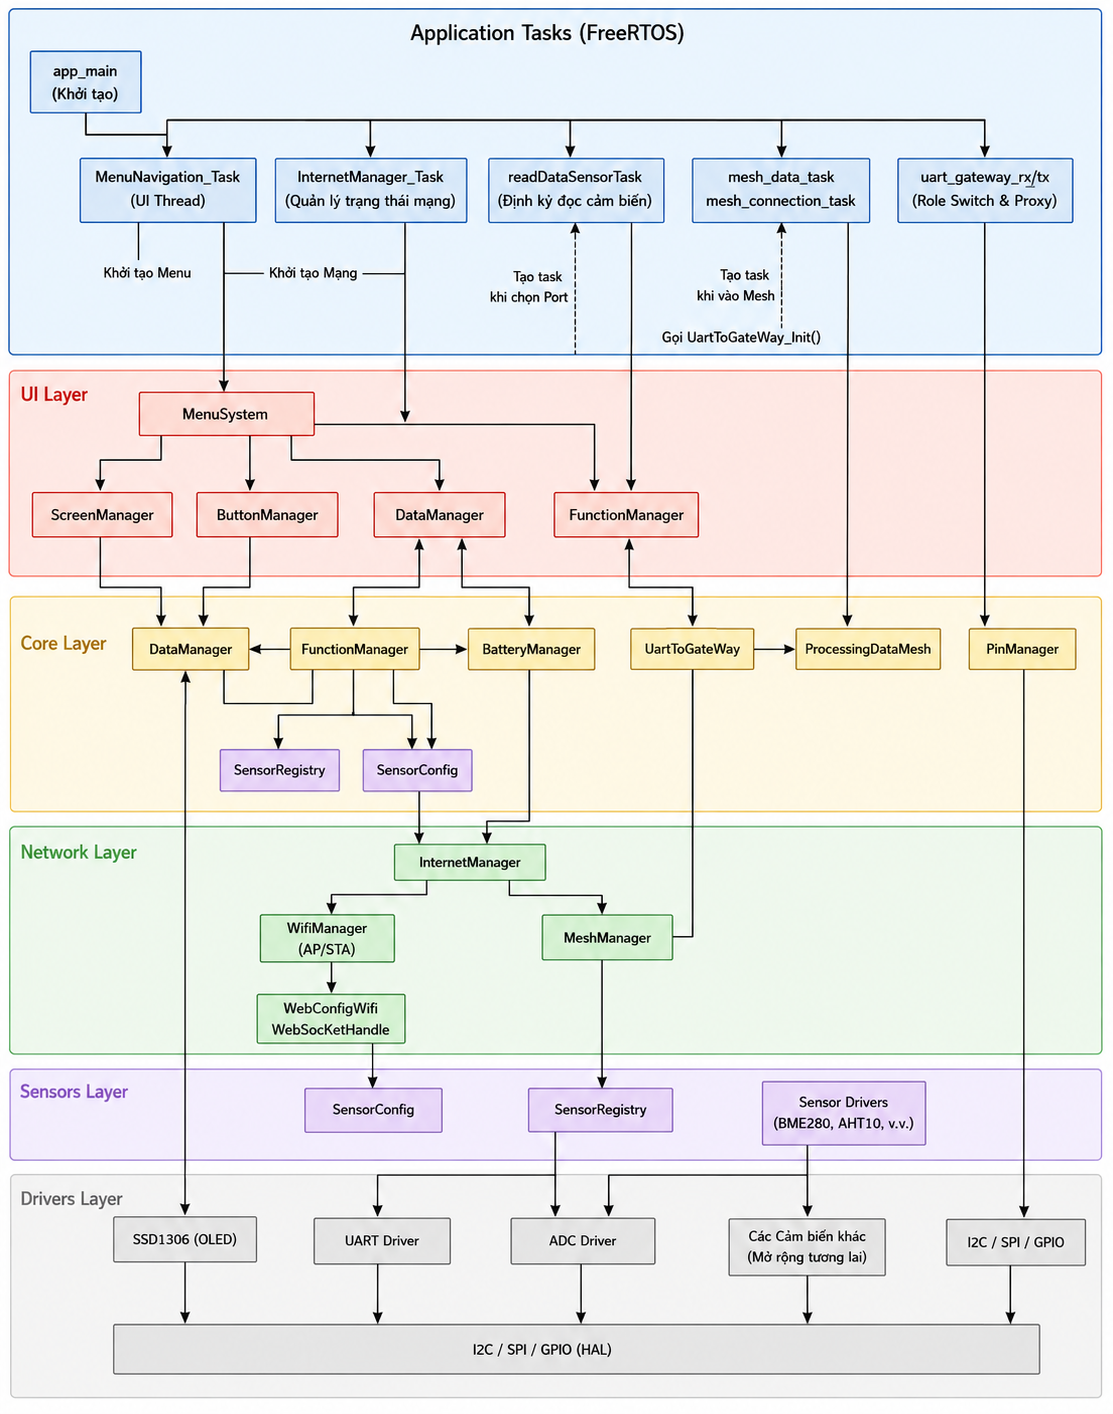
\includegraphics[width=1\textwidth]{Images/MSMS_Architecture.png}
    \captionsetup{font=small}
    \caption{Sơ đồ kiến trúc phần mềm MSMS.}
\end{figure}

\textbf{Kiến trúc phân lớp của hệ thống}

Sơ đồ mô tả kiến trúc firmware được tổ chức thành các tầng (Layer) và khối chức năng rõ ràng, đảm bảo tính đóng gói và dễ dàng mở rộng. Hệ thống bao gồm 6 thành phần chính:

\begin{enumerate}
    \item \textbf{Tầng tác vụ ứng dụng (Application Tasks):} Chạy trên nền hệ điều hành thời gian thực FreeRTOS, chịu trách nhiệm thực thi song song các luồng công việc như giao diện người dùng, đọc cảm biến, quản lý trạng thái mạng và giao tiếp UART.
    
    \item \textbf{Tầng Giao diện người dùng (UI Layer):} Chịu trách nhiệm tương tác với người dùng, bao gồm \texttt{MenuSystem} (lưu trữ cây thư mục), \texttt{ScreenManager} (hiển thị giao diện lên OLED) và \texttt{ButtonManager} (xử lý tín hiệu nút bấm vật lý).
    
    \item \textbf{Tầng Cốt lõi (Core Layer):} Nơi chứa logic trung tâm của hệ thống. Bao gồm \texttt{DataManager} (lưu trữ trạng thái toàn cục), \texttt{FunctionManager} (điều phối cảm biến và menu), \texttt{BatteryManager} (đo pin), \texttt{PinManager}, cùng với \texttt{UartToGateWay} và \texttt{ProcessingDataMesh} (chịu trách nhiệm lọc và trung chuyển dữ liệu xuống Gateway).
    
    \item \textbf{Tầng Mạng (Network Layer):} Đảm nhận các kết nối không dây. Gồm \texttt{InternetManager} (điều phối máy trạng thái mạng), \texttt{WifiManager} (kết nối AP/STA), \texttt{MeshManager} (định tuyến mạng Mesh) và khối \texttt{WebConfigWifi/WebSocKetHandle} (cung cấp Captive Portal).
    \begin{figure}[H]
        \centering
        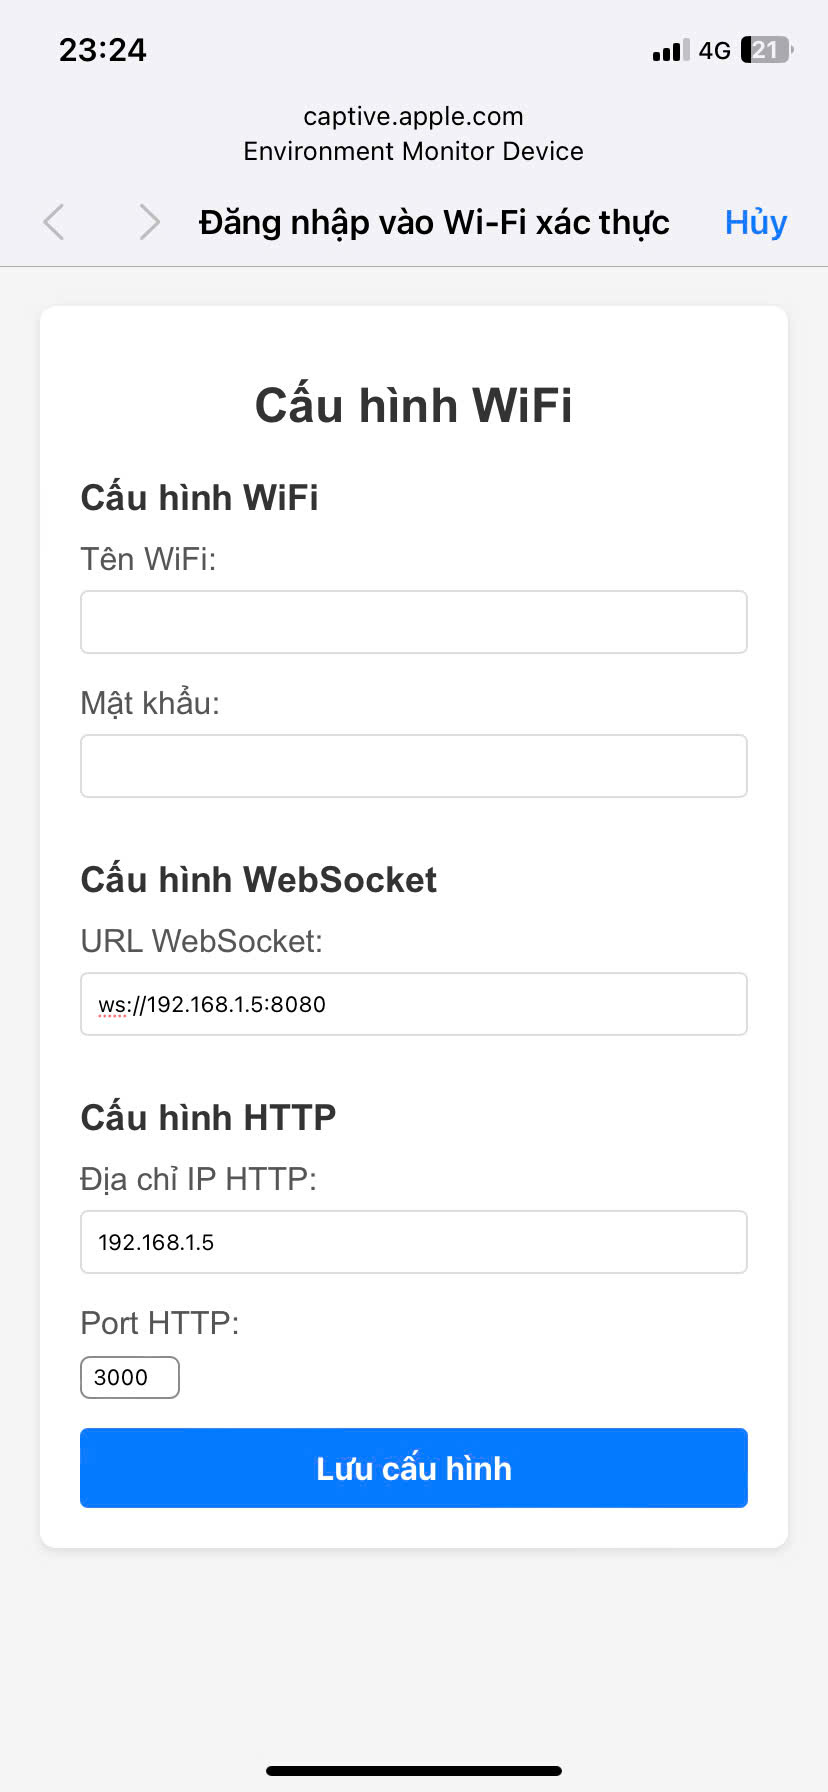
\includegraphics[width=0.5\textwidth]{Images/websever.jpg}
        \captionsetup{font=small}
        \caption{Web server (Captive Portal) cấu hình Wi-Fi cho hệ thống.}
    \end{figure}
    
    \item \textbf{Tầng Quản lý Cảm biến (Sensors Layer):} Cho phép hệ thống linh hoạt cắm rút cảm biến mà không cần biên dịch lại toàn bộ code. Chứa \texttt{SensorRegistry} (đăng ký driver), \texttt{SensorConfig} và danh sách các \texttt{Sensor Drivers} (BME280, AHT10...). Tầng này cũng được thiết kế mở để sẵn sàng đón nhận các cảm biến mới trong tương lai.
    
    \item \textbf{Tầng Trình điều khiển (Drivers Layer \& HAL):} Lớp dưới cùng giao tiếp trực tiếp với phần cứng vật lý qua chuẩn HAL (I2C, SPI, GPIO). Bao gồm driver cho màn hình \texttt{SSD1306}, \texttt{UART Driver} và \texttt{ADC Driver}.
\end{enumerate}

\textbf{Các task chính trong tầng ứng dụng}

FreeRTOS quản lý đa nhiệm với các Task tiêu biểu sau:
\begin{itemize}
    \item \textbf{\texttt{app\_main}:} Hàm khởi tạo gốc, cấp phát \texttt{DataManager} và lần lượt gọi hàm Init() của các module để sinh ra các Task bên dưới.
    \item \textbf{\texttt{MenuNavigation\_Task()}:} Vòng lặp liên tục quét trạng thái từ ButtonManager và phản hồi bằng cách vẽ lại giao diện qua ScreenManager.
    \item \textbf{\texttt{InternetManager\_Task()}:} Giám sát sự thay đổi mạng (mất kết nối, chuyển chế độ AP/STA/Mesh) để kích hoạt các callback tương ứng.
    \item \textbf{\texttt{readDataSensorTask()}:} Được sinh ra động (dynamically spawned) bởi FunctionManager mỗi khi người dùng kích hoạt đọc cảm biến trên một Port cụ thể.
    \item \textbf{\texttt{MeshTasks} (\texttt{mesh\_data} \& \texttt{mesh\_connection}):} Duy trì kết nối nội bộ giữa các Node MSMS, đóng gói dữ liệu đo lường thành JSON và truyền qua UDP.
    \item \textbf{\texttt{UARTTasks} (\texttt{uart\_rx} \& \texttt{uart\_tx}):} Nhận lệnh heartbeat từ Gateway để tự động quyết định vai trò (Role Switch) và làm proxy đẩy gói tin JSON từ mạng Mesh xuống Gateway.
\end{itemize}

\textbf{Luồng hoạt động theo vai trò mạng (Mesh Roles)}

Hệ thống MSMS hỗ trợ việc linh hoạt chuyển đổi vai trò giữa ROOT và NODE. Cụ thể, thiết bị liên tục lắng nghe giao tiếp UART từ Gateway để điều hướng các luồng thực thi:

\begin{figure}[H]
    \centering
    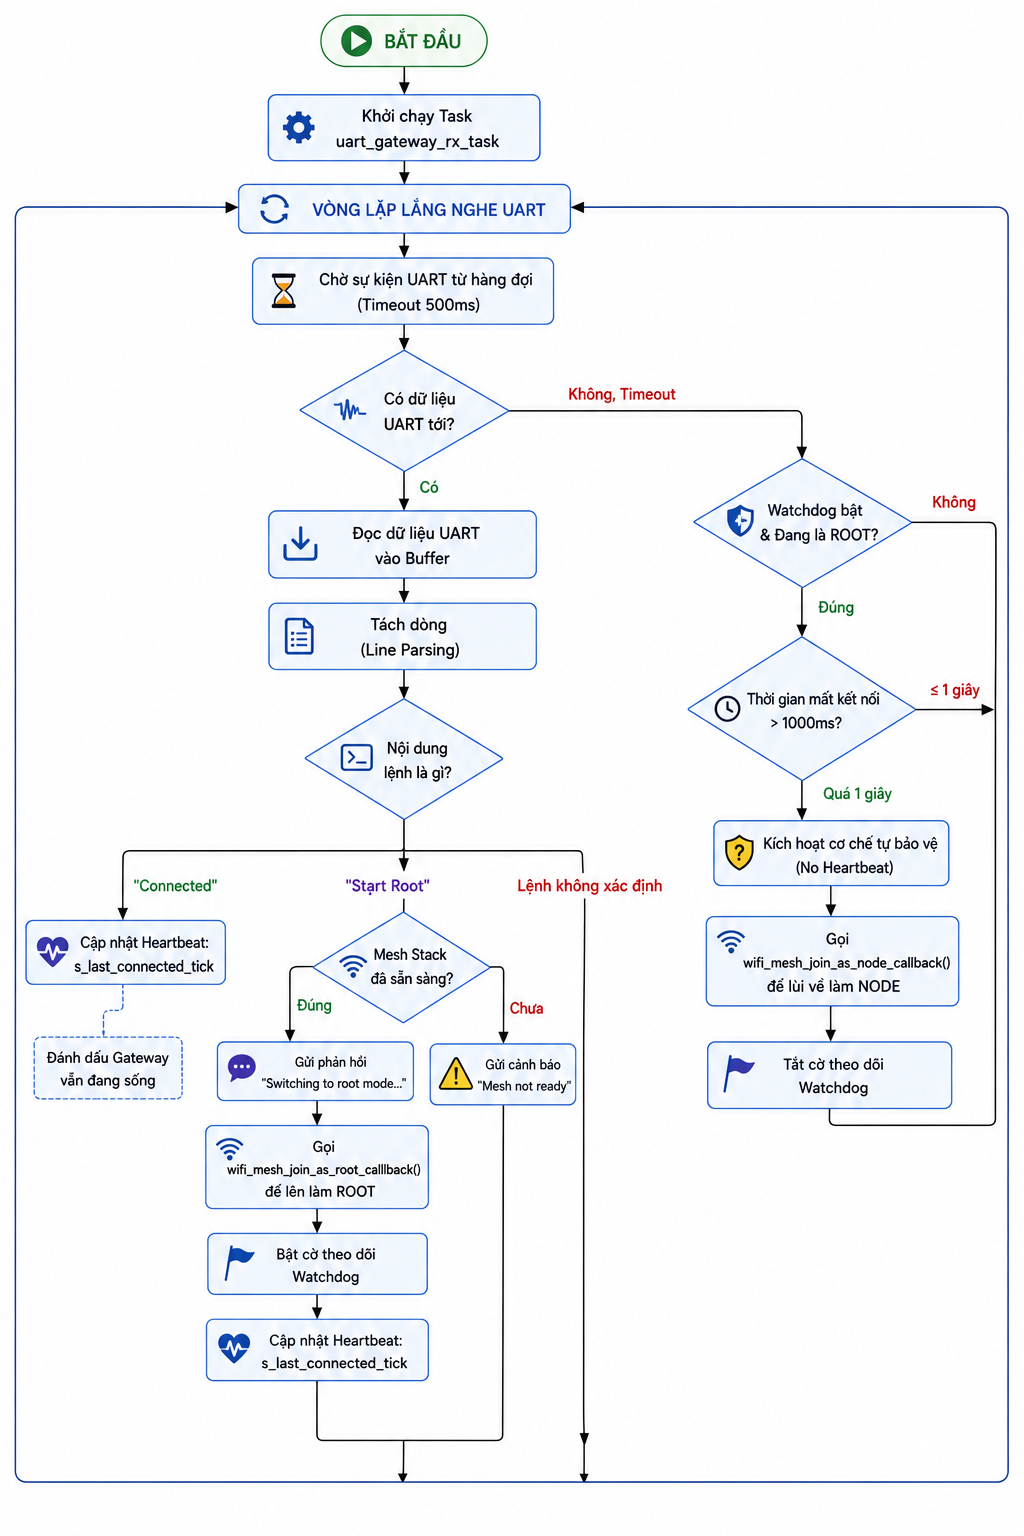
\includegraphics[width=1\textwidth]{Images/SwitchUART.png}
    \captionsetup{font=small}
    \caption{Sơ đồ chuyển đổi vai trò (Role Switch) thông qua UART.}
\end{figure}
Sơ đồ chuyển đổi vai trò mô tả cách \texttt{uart\_gateway\_rx\_task} hoạt động để quyết định cấu hình của mạch. Nếu nhận được lệnh \texttt{"Start Root"}, nó sẽ gọi \texttt{wifi\_mesh\_join\_as\_root\_callback()} để thiết lập chế độ ROOT. Đồng thời, mạch sẽ liên tục chờ nhịp tim (\texttt{"Connected"}) từ Gateway. Nếu mất kết nối với Gateway quá 1 giây trong lúc đang làm ROOT, Watchdog sẽ nổ và tự động gọi \texttt{wifi\_mesh\_join\_as\_node\_callback()} để lùi về làm NODE, đảm bảo tính an toàn và tự phục hồi cho mạng Mesh.

\begin{figure}[H]
    \centering
    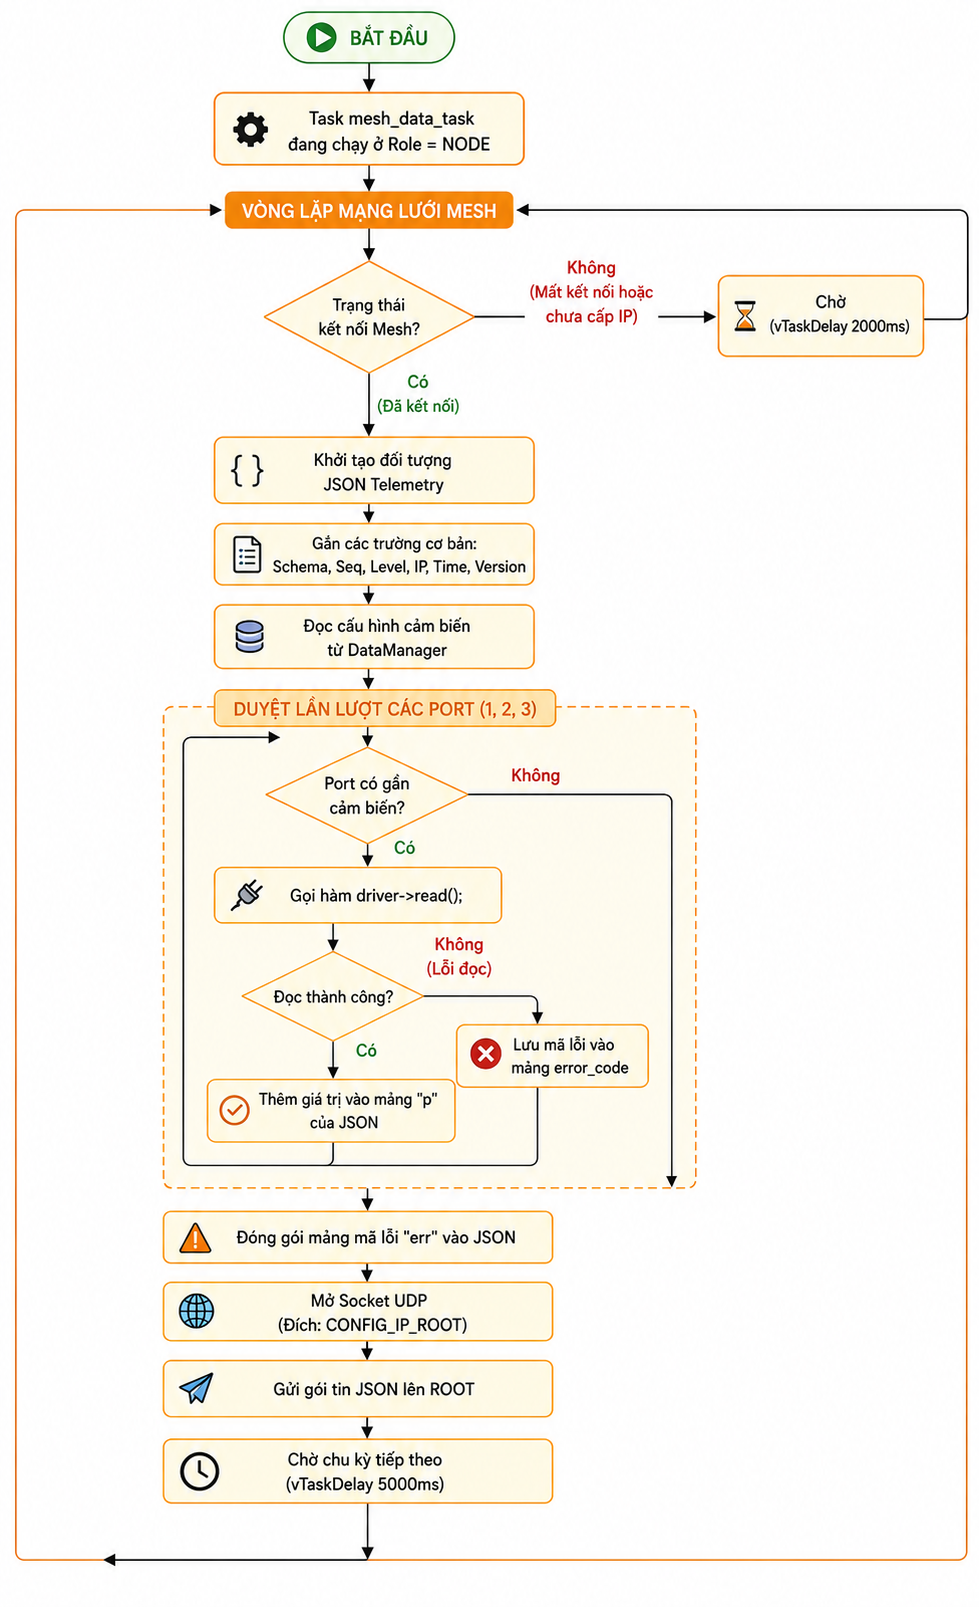
\includegraphics[width=1\textwidth]{Images/FlowNode.png}
    \captionsetup{font=small}
    \caption{Hoạt động ở trạng thái NODE.}
\end{figure}
Khi thiết bị đóng vai trò là một \textbf{NODE}, \texttt{mesh\_data\_task} sẽ lặp qua từng cổng cảm biến (Port 1, 2, 3) để gọi hàm \texttt{driver->read()}, thu thập các giá trị đo đạc và mã lỗi. Sau đó, nó đóng gói dữ liệu thành chuẩn JSON Telemetry, mở socket UDP và gửi dữ liệu này lên địa chỉ IP của mạch ROOT. Trong quá trình này, các tác vụ giao diện (Menu Navigation) vẫn hoạt động song song mượt mà trên FreeRTOS.

\begin{figure}[H]
    \centering
    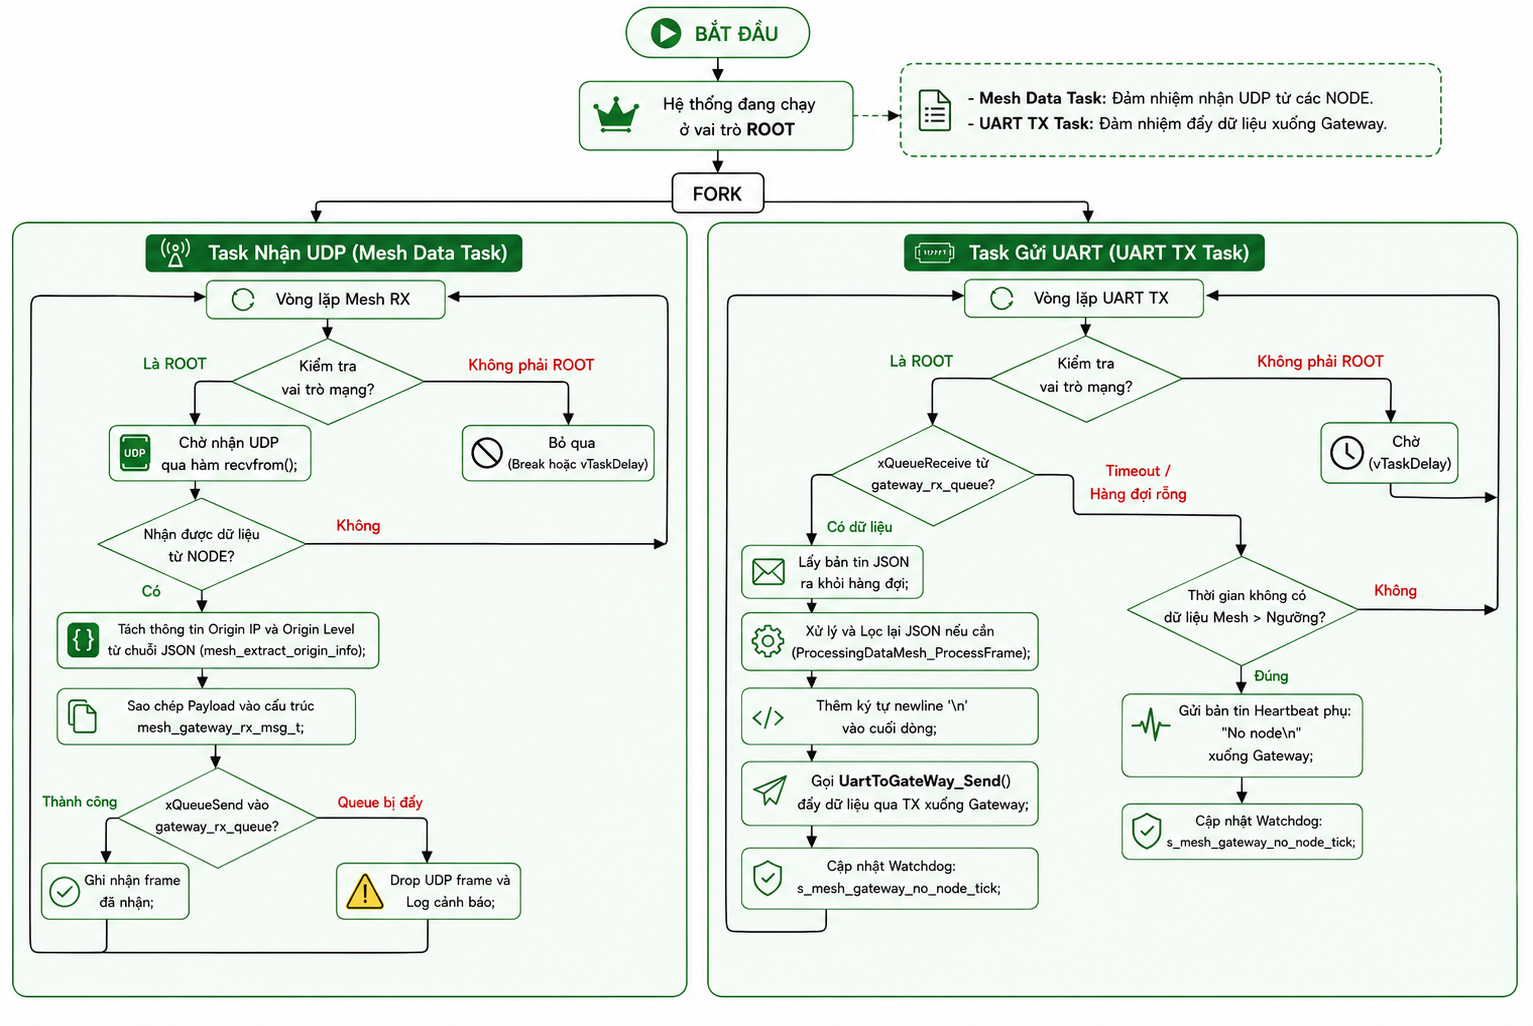
\includegraphics[width=1\textwidth]{Images/FLOW_Root.png}
    \captionsetup{font=small}
    \caption{Hoạt động ở trạng thái ROOT (Trung chuyển Dữ liệu).}
\end{figure}
Khi thiết bị đóng vai trò là \textbf{ROOT}, nó hoạt động như một cầu nối trung chuyển dữ liệu (Proxy). Mạch ngừng việc tự đọc cảm biến và thay vào đó chạy hai nhánh xử lý song song: nhánh nhận UDP sẽ liên tục lắng nghe và tiếp nhận gói tin từ các NODE con, sau đó đẩy vào hàng đợi \texttt{gateway\_rx\_queue}. Ở nhánh UART TX, thiết bị rút dữ liệu JSON từ hàng đợi này, làm sạch qua \texttt{ProcessingDataMesh\_ProcessFrame} rồi gửi thẳng xuống Gateway thông qua chuẩn UART. Nếu hàng đợi trống quá lâu, nó sẽ gửi bản tin \texttt{"No node"} xuống Gateway để báo cáo trạng thái.

\textbf{Tổng quan Wi-Fi Mesh trong hệ thống MSMS}
% TODO: Thêm hình mô tả topology mạng Wi-Fi Mesh giữa các node MSMS
\begin{figure}[H]
    \centering
    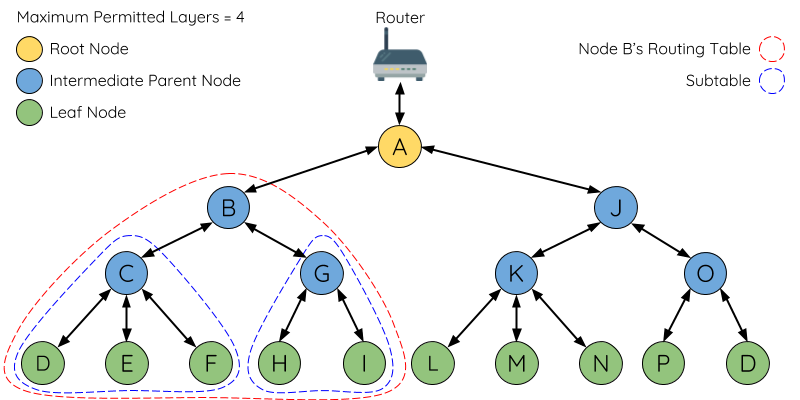
\includegraphics[width=0.8\textwidth]{Images/mesh-routing-tables.png}
    \captionsetup{font=small}
    \caption{Sơ đồ topology mạng Wi-Fi Mesh của các node MSMS.}
\end{figure}

Dự án đã triển khai thành công mạng cảm biến không dây dựa trên công nghệ \textbf{ESP-Mesh-Lite}. Thay vì bắt buộc mọi node phải kết nối trực tiếp đến một Access Point (AP) trung tâm (mô hình sao), Wi-Fi Mesh cho phép các thiết bị tự động liên kết, tạo thành một mạng lưới rộng lớn và tự khắc phục lỗi. Trong mô hình này, các thiết bị đóng vai trò như các nút trung gian, giúp mở rộng tầm phủ sóng mà không cần tăng công suất phát.

Cấu trúc mạng Mesh thực tế của hệ thống MSMS được phân cấp như sau:
\begin{itemize}
    \item \textbf{ROOT Node (Nút trung tâm)}: Đây là module MSMS được chỉ định kết nối vật lý trực tiếp với bảng mạch \textbf{Gateway} thông qua giao tiếp UART. ROOT Node đóng vai trò là điểm hội tụ dữ liệu của toàn mạng. Nó không trực tiếp đọc cảm biến mà chỉ nhận các gói tin UDP chứa dữ liệu đo lường từ các node con, sau đó làm Proxy chuyển tiếp (forward) toàn bộ luồng dữ liệu này xuống Gateway.
    \item \textbf{Intermediate/Leaf Nodes (Nút đo lường)}: Các module MSMS được phân bố ở nhiều vị trí không gian khác nhau. Chúng thực hiện chức năng lấy mẫu cảm biến theo cấu hình riêng của từng trạm (Port 1, 2, 3), đóng gói dữ liệu thành chuẩn JSON (bao gồm địa chỉ IP nguồn, mức định tuyến, MAC và dữ liệu các đại lượng), rồi truyền qua giao thức mạng UDP hướng thẳng về địa chỉ IP của ROOT Node. Các node ở quá xa ROOT sẽ tự động kết nối và truyền dữ liệu bắc cầu qua các node trung gian (hop).
\end{itemize}

Luồng dữ liệu thực tế đang chạy trong mạng:
\begin{enumerate}
    \item Mỗi \textbf{NODE} (lá hoặc trung gian) lấy mẫu cảm biến, đóng gói thành gói tin JSON Telemetry hoàn chỉnh.
    \item \textbf{NODE} mở kết nối Socket UDP và bắn gói tin này ngược lên địa chỉ IP của \textbf{ROOT}.
    \item Mạch \textbf{ROOT} nhận gói tin UDP, bóc tách thông tin định tuyến (Origin IP, MAC) và đưa JSON vào hàng đợi \texttt{gateway\_rx\_queue}.
    \item Mạch \textbf{ROOT} rút JSON từ hàng đợi, xử lý làm sạch và truyền thẳng xuống \textbf{Gateway} thông qua giao tiếp UART tốc độ cao.
    \item \textbf{Gateway} phân tích dữ liệu, hiển thị lên màn hình đồ họa lớn và lưu trữ toàn cục vào thẻ nhớ SD.
\end{enumerate}

\paragraph{B. Thiết kế Firmware Gateway} \mbox{}\\

Firmware của Gateway đóng vai trò là bộ não điều phối trung tâm của toàn bộ hệ thống. Nhiệm vụ chính của nó là nhận luồng dữ liệu thô qua UART từ MSMS ROOT, xử lý, lưu trữ, và hiển thị giao diện đồ họa (GUI) cho người dùng thông qua màn hình cảm ứng.

\textbf{Kiến trúc phần mềm Gateway}

\begin{figure}[H]
    \centering
    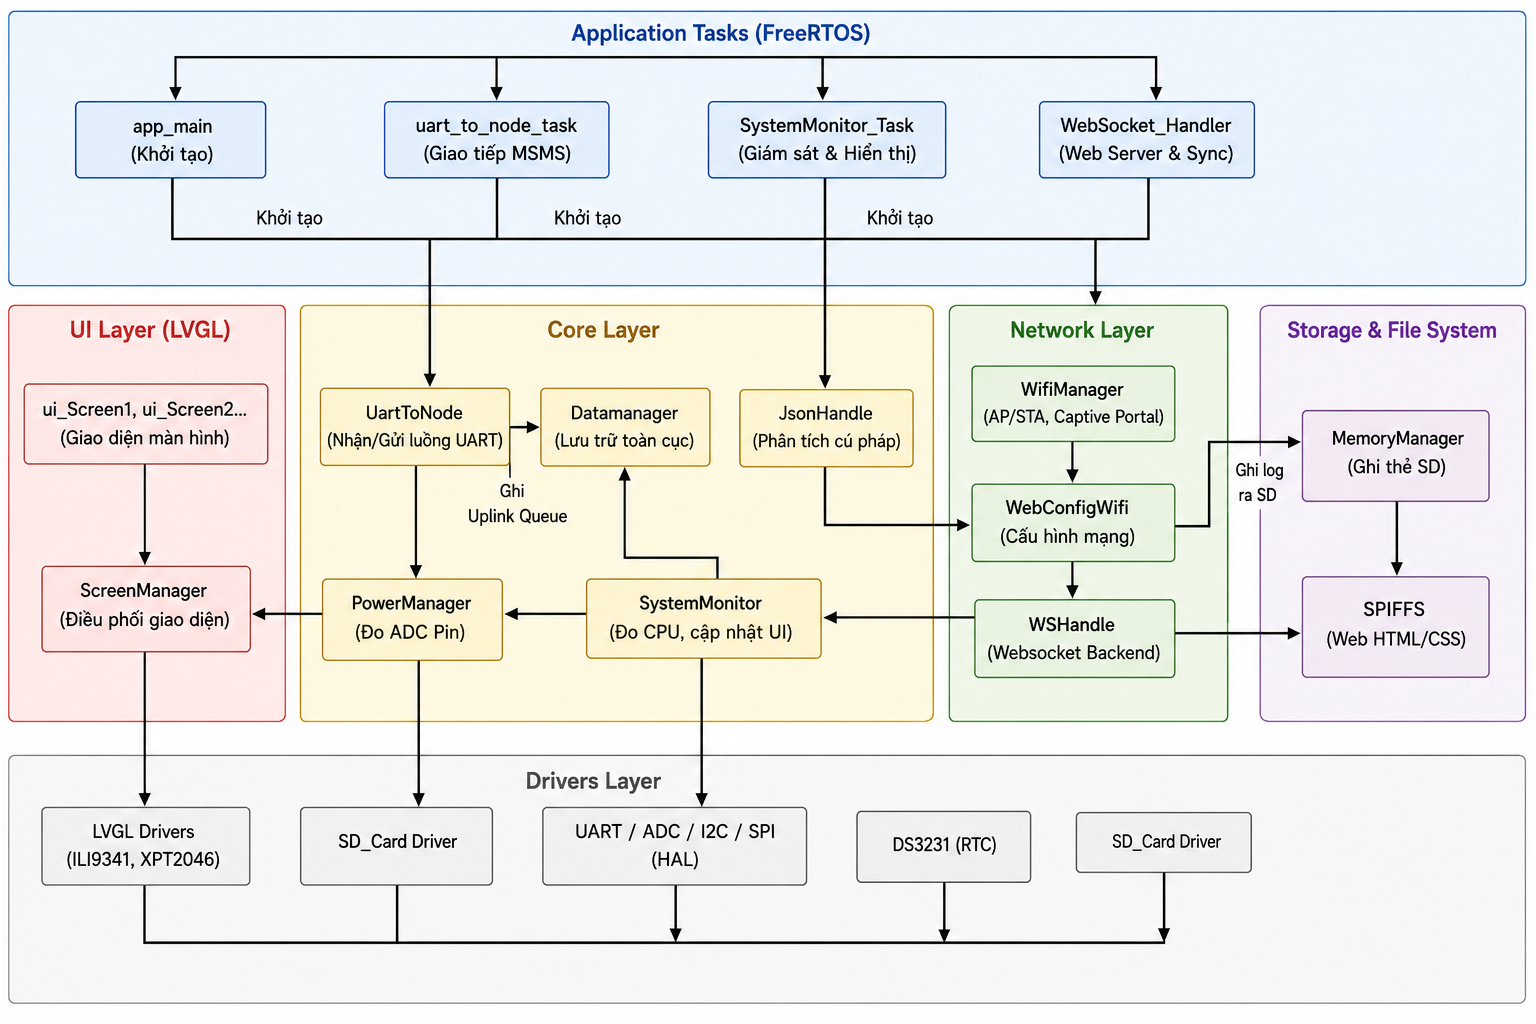
\includegraphics[width=1\textwidth]{Images/Gateway_Architecture.png}
    \captionsetup{font=small}
    \caption{Sơ đồ kiến trúc phần mềm Gateway.}
\end{figure}

Tương tự như Node MSMS, firmware Gateway cũng được thiết kế phân lớp để đảm bảo khả năng mở rộng:
\begin{enumerate}
    \item \textbf{Tầng tác vụ ứng dụng (Application Tasks):} Điều phối hệ thống thông qua các Task của FreeRTOS, bao gồm quản lý UART, hiển thị màn hình, và xử lý kết nối Web.
    \item \textbf{Tầng Giao diện (UI Layer):} Chứa các logic đồ họa dựa trên thư viện \textbf{LVGL}, bao gồm \texttt{ScreenManager} đóng vai trò điều phối các màn hình hiển thị trực quan (số liệu đo đạc, biểu đồ, phần trăm pin).
    \item \textbf{Tầng Cốt lõi (Core Layer):} Xử lý logic trung tâm. Bao gồm \texttt{Datamanager} (lưu cấu trúc dữ liệu toàn cục), \texttt{JsonHandle} (phân tích chuỗi dữ liệu JSON gửi lên từ mạng Mesh), và \texttt{SystemMonitor} (giám sát tài nguyên phần cứng như CPU, đo ADC pin).
    \item \textbf{Tầng Mạng (Network Layer):} Cung cấp tính năng Web Server và \texttt{WSHandle} (WebSocket) cho phép theo dõi dữ liệu cảm biến trực tiếp theo thời gian thực qua trình duyệt.
    \item \textbf{Tầng Lưu trữ (Storage \& File System):} Đóng vai trò cực kỳ quan trọng, sử dụng \texttt{MemoryManager} để ghi nối tiếp log (dưới dạng JSON/CSV) vào thẻ nhớ SD, và \texttt{SPIFFS} lưu các tệp tin tĩnh (HTML/CSS) hỗ trợ Web UI.
    \item \textbf{Tầng Trình điều khiển (Drivers Layer):} Chứa các thư viện bậc thấp tương tác với vi mạch phần cứng như \texttt{DS3231} (RTC), giao tiếp màn hình TFT (qua SPI/I2C) và SD Card.
\end{enumerate}

\textbf{Luồng hoạt động chính của Gateway}

Để xử lý khối lượng lớn công việc mà không bị nghẽn (non-blocking), Gateway chạy 3 luồng công việc (Task) trên nền FreeRTOS thực thi hoàn toàn song song:

\begin{figure}[H]
    \centering
    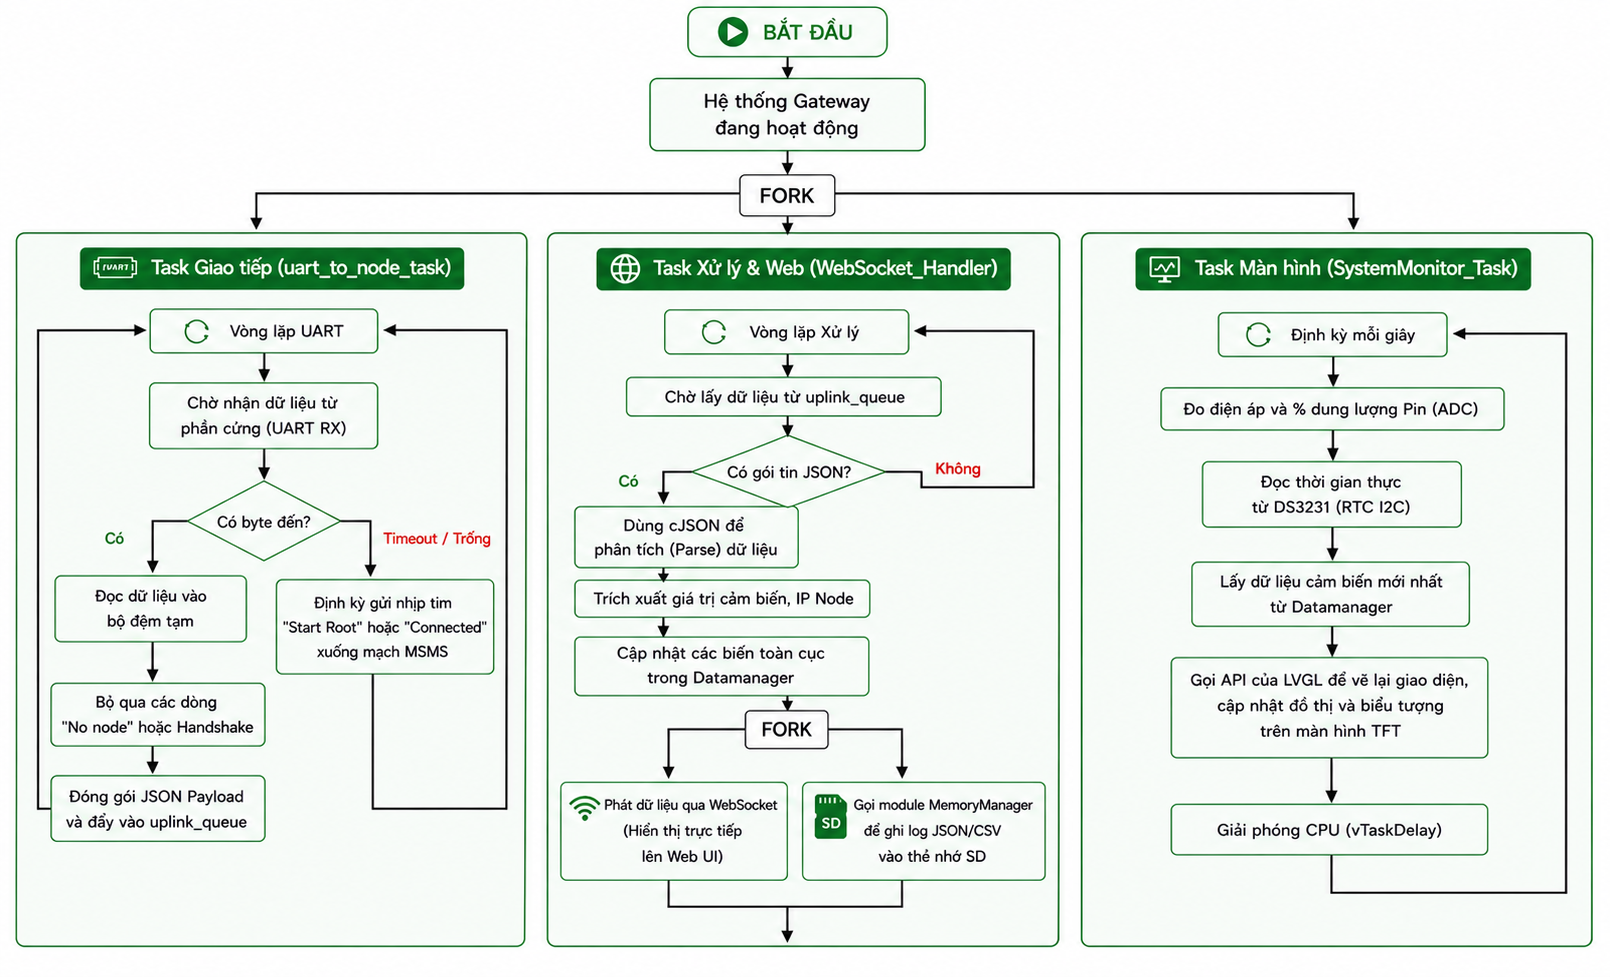
\includegraphics[width=1\textwidth]{Images/FlowGateWay.png}
    \captionsetup{font=small}
    \caption{Lưu đồ hoạt động trung tâm của Gateway.}
\end{figure}

\begin{itemize}
    \item \textbf{Task Giao tiếp (\texttt{uart\_to\_node\_task}):} Luôn chạy ngầm để trao đổi "Nhịp tim" (gửi bản tin định kỳ \texttt{Start Root} / \texttt{Connected}) với board ROOT qua UART. Task này liên tục hứng dòng byte gửi lên, lọc bỏ các dòng tin báo trạng thái kết nối, bóc tách đoạn payload mang cấu trúc JSON chuẩn và đẩy thẳng vào hàng đợi \texttt{uplink\_queue}.
    \item \textbf{Task Xử lý \& Mạng (\texttt{WebSocket\_Handler}):} Thường trực đọc dữ liệu từ \texttt{uplink\_queue}. Khi có tin đến, nó dùng bộ phân tích \texttt{cJSON} để đọc các giá trị. Từng thông số (nhiệt độ, độ ẩm...) của mỗi Node sẽ được bóc tách và đổ vào \texttt{Datamanager}. Song song đó, Task này sẽ gọi module để ghi dữ liệu ra thẻ SD, đồng thời phát quảng bá (broadcast) bản tin này tới tất cả các client đang theo dõi trên Web UI thông qua WebSocket.
    \item \textbf{Task Màn hình (\texttt{SystemMonitor\_Task}):} Chịu trách nhiệm trực quan hóa dữ liệu cục bộ. Cứ mỗi 1 giây, hệ thống quét module \texttt{DS3231} để lấy giờ chuẩn xác, đo mức điện áp pin cấp cho Gateway, và gọi các API của LVGL để làm mới (refresh) giao diện hiển thị. Việc tách biệt luồng này đảm bảo màn hình luôn được thao tác mượt mà ngay cả khi đường truyền UART hoặc mạng Mesh đang tắc nghẽn.
\end{itemize}
\paragraph{C. Thiết kế Software (Web Dashboard \& Mobile App)} \mbox{}\\

Bên cạnh firmware chạy trên vi điều khiển, hệ thống còn được phát triển kèm theo một hệ sinh thái phần mềm hoàn chỉnh bao gồm Server trung tâm, Web Dashboard và Mobile App nhằm mục đích giám sát, điều khiển và lưu trữ dữ liệu tập trung.

\textbf{Kiến trúc phần mềm hệ sinh thái}

\begin{figure}[H]
    \centering
    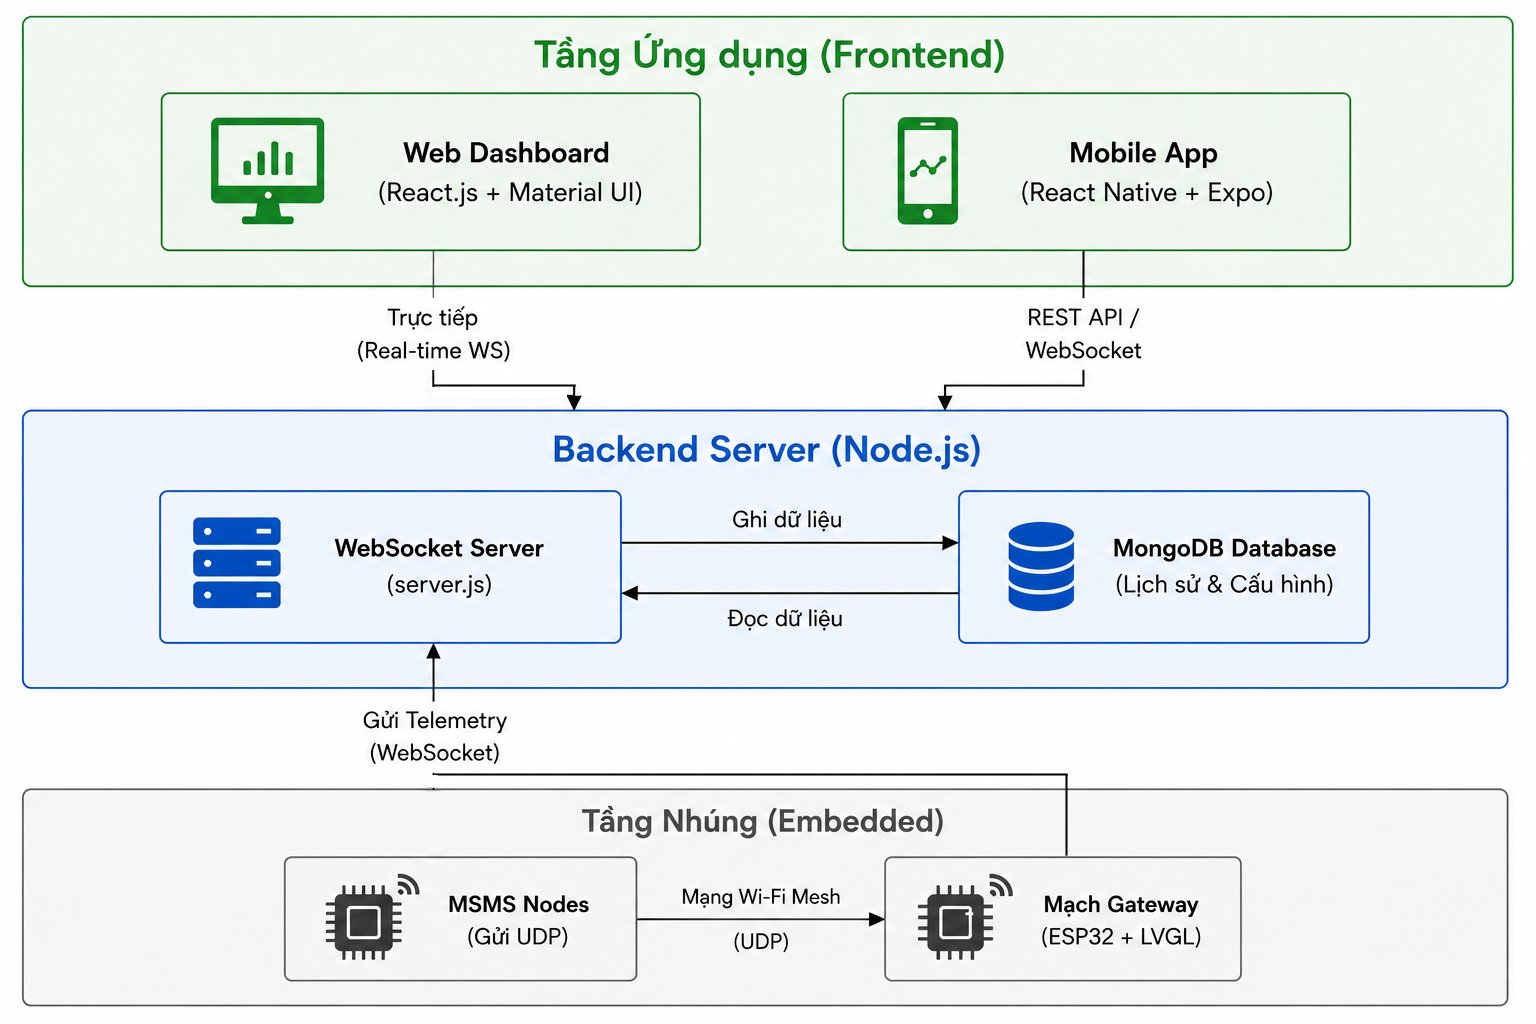
\includegraphics[width=0.8\textwidth]{Images/Software_Architecture.png}
    \captionsetup{font=small}
    \caption{Sơ đồ kiến trúc phần mềm (Web Dashboard \& Mobile App).}
\end{figure}

Hệ thống được chia thành 3 khối chính:
\begin{enumerate}
    \item \textbf{Backend Server (Node.js \& MongoDB):}
    \begin{itemize}
        \item Cốt lõi của Backend là một máy chủ \textbf{WebSocket Server} viết bằng Node.js (\texttt{server.js}). Máy chủ này làm nhiệm vụ lắng nghe kết nối liên tục từ mạch Gateway. 
        \item Khi Gateway đẩy các gói tin Telemetry (nhận từ UART) lên thông qua WebSocket, Backend sẽ bóc tách JSON, phân loại theo địa chỉ IP/MAC của từng Node và lưu lịch sử đo đạc vào cơ sở dữ liệu \textbf{MongoDB}.
        \item Đồng thời, Backend cũng đóng vai trò là trạm trung chuyển (broadcast), lập tức đẩy dữ liệu real-time tới tất cả các client đang kết nối (Web/App).
    \end{itemize}
    
    \item \textbf{Web Dashboard (React.js):}
    \begin{itemize}
        \item Được xây dựng trên nền tảng \textbf{React.js} kết hợp với bộ giao diện \textbf{Material UI} (phiên bản Vision UI Dashboard).
        \item Giao diện hiển thị trực quan các biểu đồ (Line chart, Bar chart) thông qua thư viện \textbf{ApexCharts}, vẽ lại ngay lập tức trạng thái nhiệt độ, độ ẩm, nồng độ bụi mịn PM2.5/PM10, CO2, v.v. của toàn bộ các trạm trong mạng Mesh.
    \end{itemize}
    
    \item \textbf{Mobile App (React Native):}
    \begin{itemize}
        \item Ứng dụng di động được lập trình bằng \textbf{React Native} và khung làm việc \textbf{Expo}.
        \item Quản lý trạng thái nội bộ bằng thư viện \textbf{Zustand} và sử dụng \textbf{React Query} để đồng bộ lịch sử dữ liệu từ Server. Nhờ tích hợp WebSocket, người dùng có thể mở điện thoại ra và xem các chỉ số an toàn môi trường một cách mượt mà và linh hoạt.
    \end{itemize}
\end{enumerate}
\newpage

\section*{CHƯƠNG 4. KIỂM THỬ HỆ THỐNG VÀ LẤY DỮ LIỆU}
\addcontentsline{toc}{section}{\numberline{}CHƯƠNG 4. KIỂM THỬ HỆ THỐNG VÀ LẤY DỮ LIỆU}
\setcounter{section}{4}
\setcounter{subsection}{0}
\setcounter{figure}{0}
\setcounter{table}{0}

\subsection{Chiến lược kiểm thử}

Để đánh giá tính ổn định và khả năng mở rộng của hệ thống, quy trình kiểm thử được chia thành 4 giai đoạn chính:
\begin{itemize}
    \item \textbf{Kiểm thử cục bộ Node MSMS}: Đánh giá phần cứng, cảm biến, giao diện OLED và khả năng truyền UDP.
    \item \textbf{Kiểm thử cục bộ Gateway}: Kiểm tra màn hình TFT, đồng hồ RTC, thẻ nhớ SD và năng lực xử lý JSON.
    \item \textbf{Kiểm thử Software (Web \& App)}: Kiểm tra giao diện người dùng, kết nối WebSocket và cơ sở dữ liệu MongoDB.
    \item \textbf{Kiểm thử tích hợp toàn hệ thống (End-to-End Test)}: Chạy đồng thời toàn bộ mạng Mesh, truyền dữ liệu từ cảm biến lên tận Web Dashboard và xác minh tính toàn vẹn của dữ liệu.
\end{itemize}

\subsection{Kiểm thử mạch Node MSMS}

\subsubsection{Kiểm thử phần cứng \& Cảm biến}
\begin{itemize}
    \item \textbf{Mục tiêu}: Đảm bảo nguồn 3.3V/5V ổn định, các nút bấm (BACK, SELECT, MOVE) không bị dội phím (debounce tốt).
    \item \textbf{Quy trình}: Cấp nguồn qua module IP5306, sử dụng đồng hồ vạn năng đo áp. Cắm các cảm biến BME280 (I2C) và cảm biến MQ (Analog) vào các Port.
    \item \textbf{Kết quả}: Điện áp duy trì ở mức 3.3V cho MCU và 5V cho cảm biến khí. Các nút bấm phản hồi chính xác, không ghi nhận hiện tượng chạm chập hay nhấn đúp. Cảm biến đọc dữ liệu liên tục không bị treo đường truyền I2C.
\end{itemize}

\subsubsection{Kiểm thử Firmware (Menu \& Mesh UDP)}
\begin{itemize}
    \item \textbf{Mục tiêu}: Trình điều khiển OLED SSD1306 hiển thị mượt mà; mạch MSMS có khả năng chuyển đổi vai trò (Role Switch) và gửi UDP thành công.
    \item \textbf{Quy trình}: Sử dụng menu trên OLED để chuyển đổi cấu hình Port cảm biến. Cấp lệnh UART \texttt{"Start Root"} để kiểm tra khả năng tự động chuyển vai trò thành ROOT.
    \item \textbf{Kết quả}: Giao diện OLED phản hồi tức thời. Thiết bị MSMS tự động phân mảnh mạng Mesh thành công: Node con đọc dữ liệu và gửi UDP chính xác tới địa chỉ IP của Node ROOT mà không bị rớt gói tin trong khoảng cách 15m (không vật cản).
\end{itemize}

\subsection{Kiểm thử mạch Gateway}

\subsubsection{Kiểm thử Màn hình TFT (LVGL) \& Giao tiếp UART}
\begin{itemize}
    \item \textbf{Mục tiêu}: Màn hình lớn TFT hiển thị đúng đồ họa LVGL; mạch Gateway nhận đủ và đúng dữ liệu JSON qua cổng UART tốc độ cao.
    \item \textbf{Quy trình}: Viết script giả lập gửi dữ liệu JSON (đóng giả mạch ROOT) qua cổng UART vào Gateway với tần suất 1 giây/lần.
    \item \textbf{Kết quả}: Module \texttt{uart\_to\_node\_task} của Gateway bóc tách JSON chính xác 100\%, không bị tràn bộ đệm (buffer overflow). Task \texttt{SystemMonitor} cập nhật số liệu lên màn hình TFT mượt mà, không xảy ra hiện tượng nhấp nháy hay giật lag.
\end{itemize}

\subsubsection{Kiểm thử RTC DS3231 \& Thẻ nhớ SD}
\begin{itemize}
    \item \textbf{Mục tiêu}: Thời gian thực được lưu chính xác khi mất điện; dữ liệu JSON được ghi thành file log hợp lệ vào thẻ nhớ.
    \item \textbf{Kết quả}: Gắn pin CMOS cho mạch RTC, sau khi ngắt nguồn 24h mạch vẫn cập nhật đúng giờ. Các file log CSV/JSON được tạo tự động trên thẻ nhớ SD với đầy đủ payload cảm biến và mốc thời gian (Timestamp).
\end{itemize}

\subsection{Kiểm thử Hệ sinh thái Software (Web Dashboard \& Mobile App)}

\subsubsection{Kiểm thử Web Dashboard \& WebSocket Server}
\begin{itemize}
    \item \textbf{Mục tiêu}: Đảm bảo Web Dashboard vẽ lại biểu đồ ngay lập tức (Real-time) khi có dữ liệu mới.
    \item \textbf{Quy trình}: Mở Backend Node.js và Web React.js. Gửi 1000 gói tin JSON mô phỏng biến động nhiệt độ từ $25^\circ C$ đến $35^\circ C$ liên tục trong 1 phút vào WebSocket Server.
    \item \textbf{Kết quả}: Server Node.js lưu trữ toàn bộ 1000 bản ghi vào MongoDB thành công. Trình duyệt Web React.js render các biểu đồ ApexCharts trơn tru, hiển thị sự thay đổi nhiệt độ theo thời gian thực với độ trễ (latency) dưới 50ms.
\end{itemize}

\subsubsection{Kiểm thử Mobile App (React Native)}
\begin{itemize}
    \item \textbf{Kết quả}: Ứng dụng điện thoại kết nối trơn tru tới REST API của Backend. Thư viện Zustand giữ trạng thái dữ liệu (State) đồng bộ với Web Dashboard. Giao diện thân thiện và hiển thị tốt trên cả nền tảng Android.
\end{itemize}

\subsection{Kiểm thử tích hợp toàn hệ thống (End-to-End Test)}

Bài test kiểm chứng toàn bộ quy trình: \textbf{Môi trường $\rightarrow$ Cảm biến $\rightarrow$ NODE $\rightarrow$ ROOT $\rightarrow$ Gateway $\rightarrow$ Server $\rightarrow$ Web/App}.

\begin{enumerate}
    \item \textbf{Thiết lập}: Bố trí 2 mạch MSMS (1 đóng vai trò NODE, 1 đóng vai trò ROOT nối với Gateway). Bật Web Dashboard trên PC.
    \item \textbf{Thực thi}: Đặt một ly nước nóng (hoặc hơi sương) lại gần cảm biến BME280 tại mạch NODE.
    \item \textbf{Quan sát luồng dữ liệu}:
    \begin{itemize}
        \item Màn hình OLED của NODE hiển thị độ ẩm tăng dần từ $60\%$ lên $85\%$.
        \item NODE tự động đóng gói số liệu $85\%$, gửi UDP tới ROOT.
        \item ROOT nhận UDP, đẩy qua UART xuống Gateway.
        \item Gateway tiếp nhận JSON qua UART, hiển thị $85\%$ lên màn hình TFT và lưu thẻ nhớ SD.
        \item Gateway đẩy số liệu lên WebSocket Server.
        \item Web Dashboard vẽ một đường dốc đứng vọt lên mức $85\%$ trên biểu đồ độ ẩm. Điện thoại rung cảnh báo (nếu có cài ngưỡng).
    \end{itemize}
    \item \textbf{Kết quả}: Hệ thống hoạt động hoàn hảo từ đầu cuối này đến đầu cuối kia (End-to-End). Dữ liệu nhất quán tại mọi điểm hiển thị (OLED, TFT, Web, App). Độ trễ từ lúc cảm biến nhận hơi ẩm đến lúc đồ thị trên Web nhảy lên chỉ rơi vào khoảng \textbf{300ms - 500ms}.
\end{enumerate}

\begin{figure}[H]
    \centering
    \begin{minipage}[t]{0.32\textwidth}
        \centering
        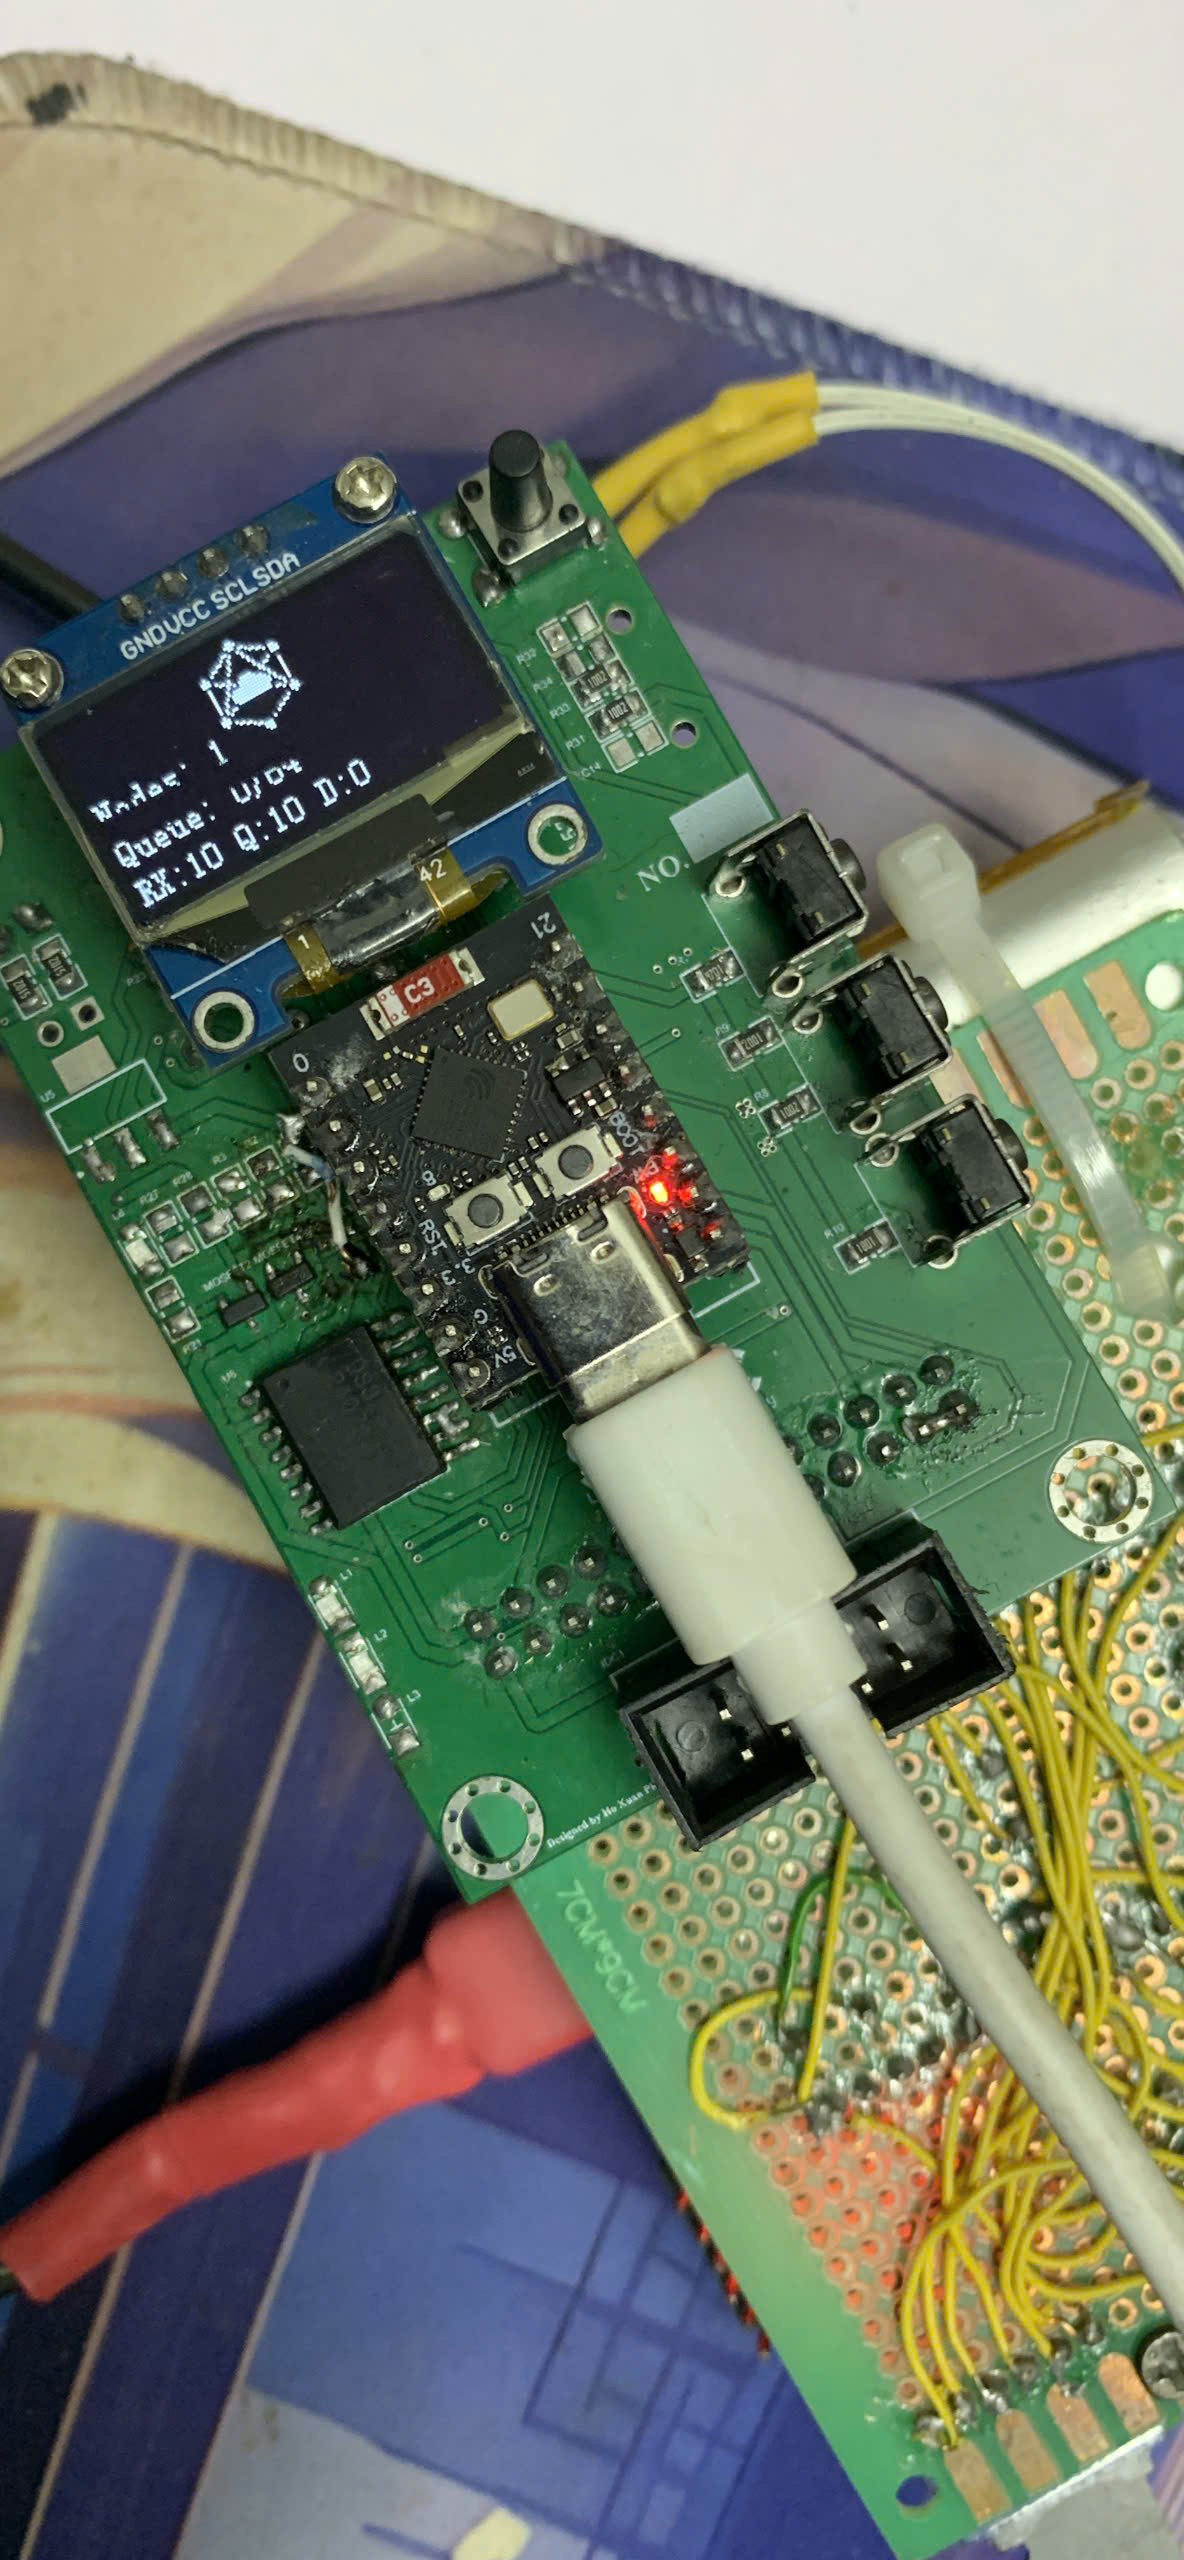
\includegraphics[width=\linewidth]{Images/setup1.jpg}
        \caption*{Mạch Node MSMS}
    \end{minipage}\hfill
    \begin{minipage}[t]{0.32\textwidth}
        \centering
        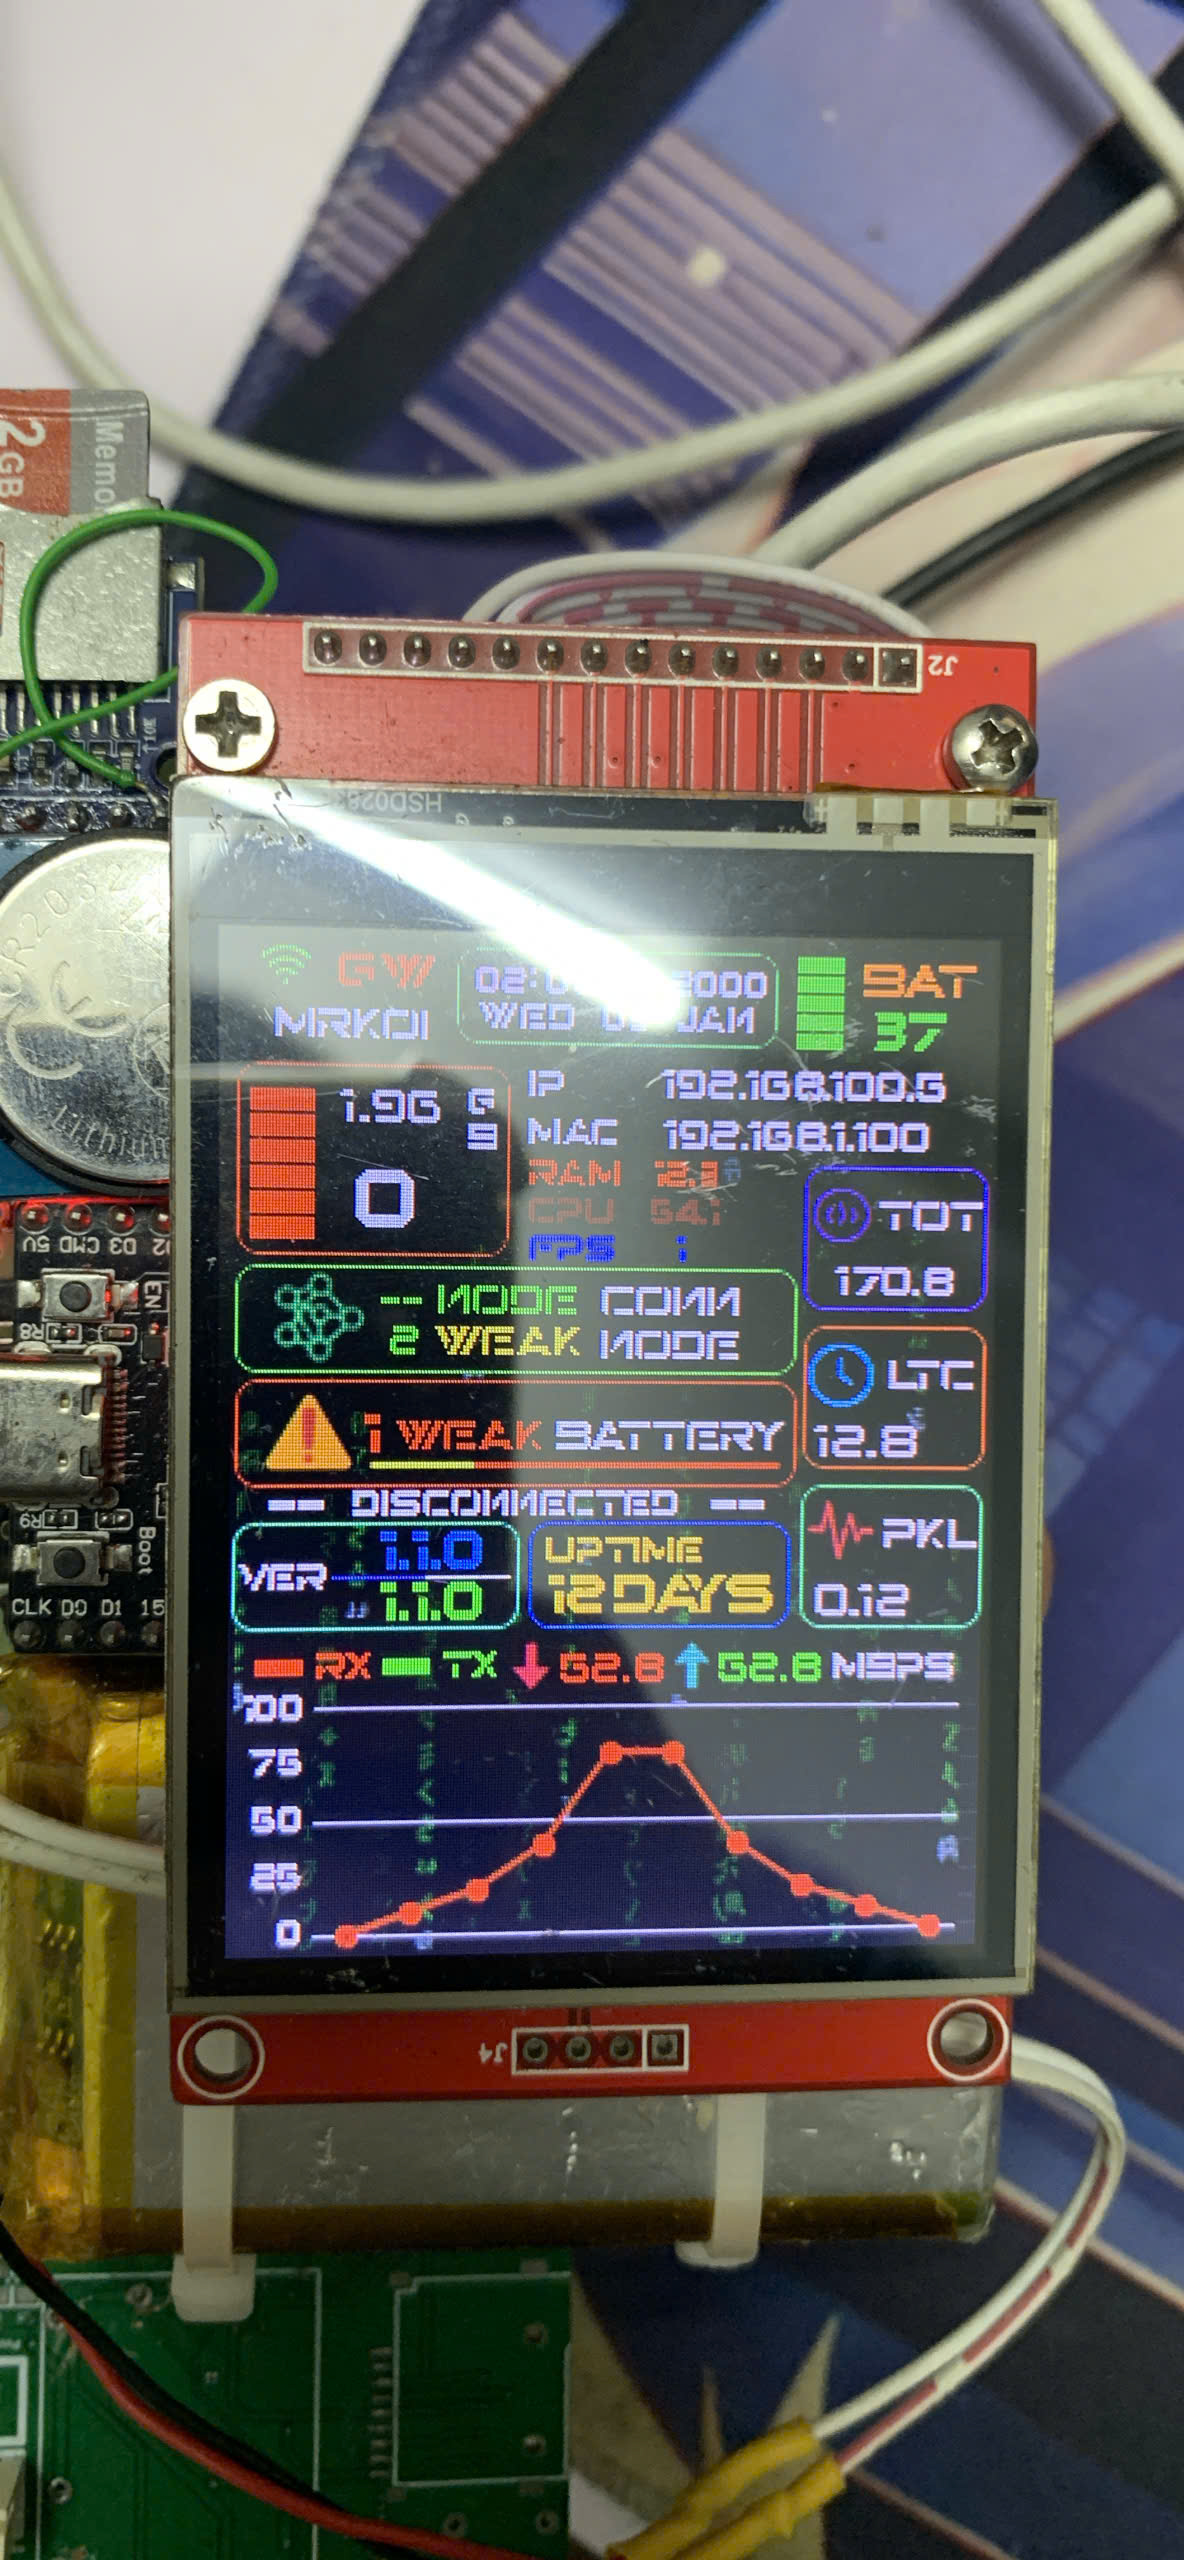
\includegraphics[width=\linewidth]{Images/setup2.jpg}
        \caption*{Trạm Gateway thu thập}
    \end{minipage}\hfill
    \begin{minipage}[t]{0.32\textwidth}
        \centering
        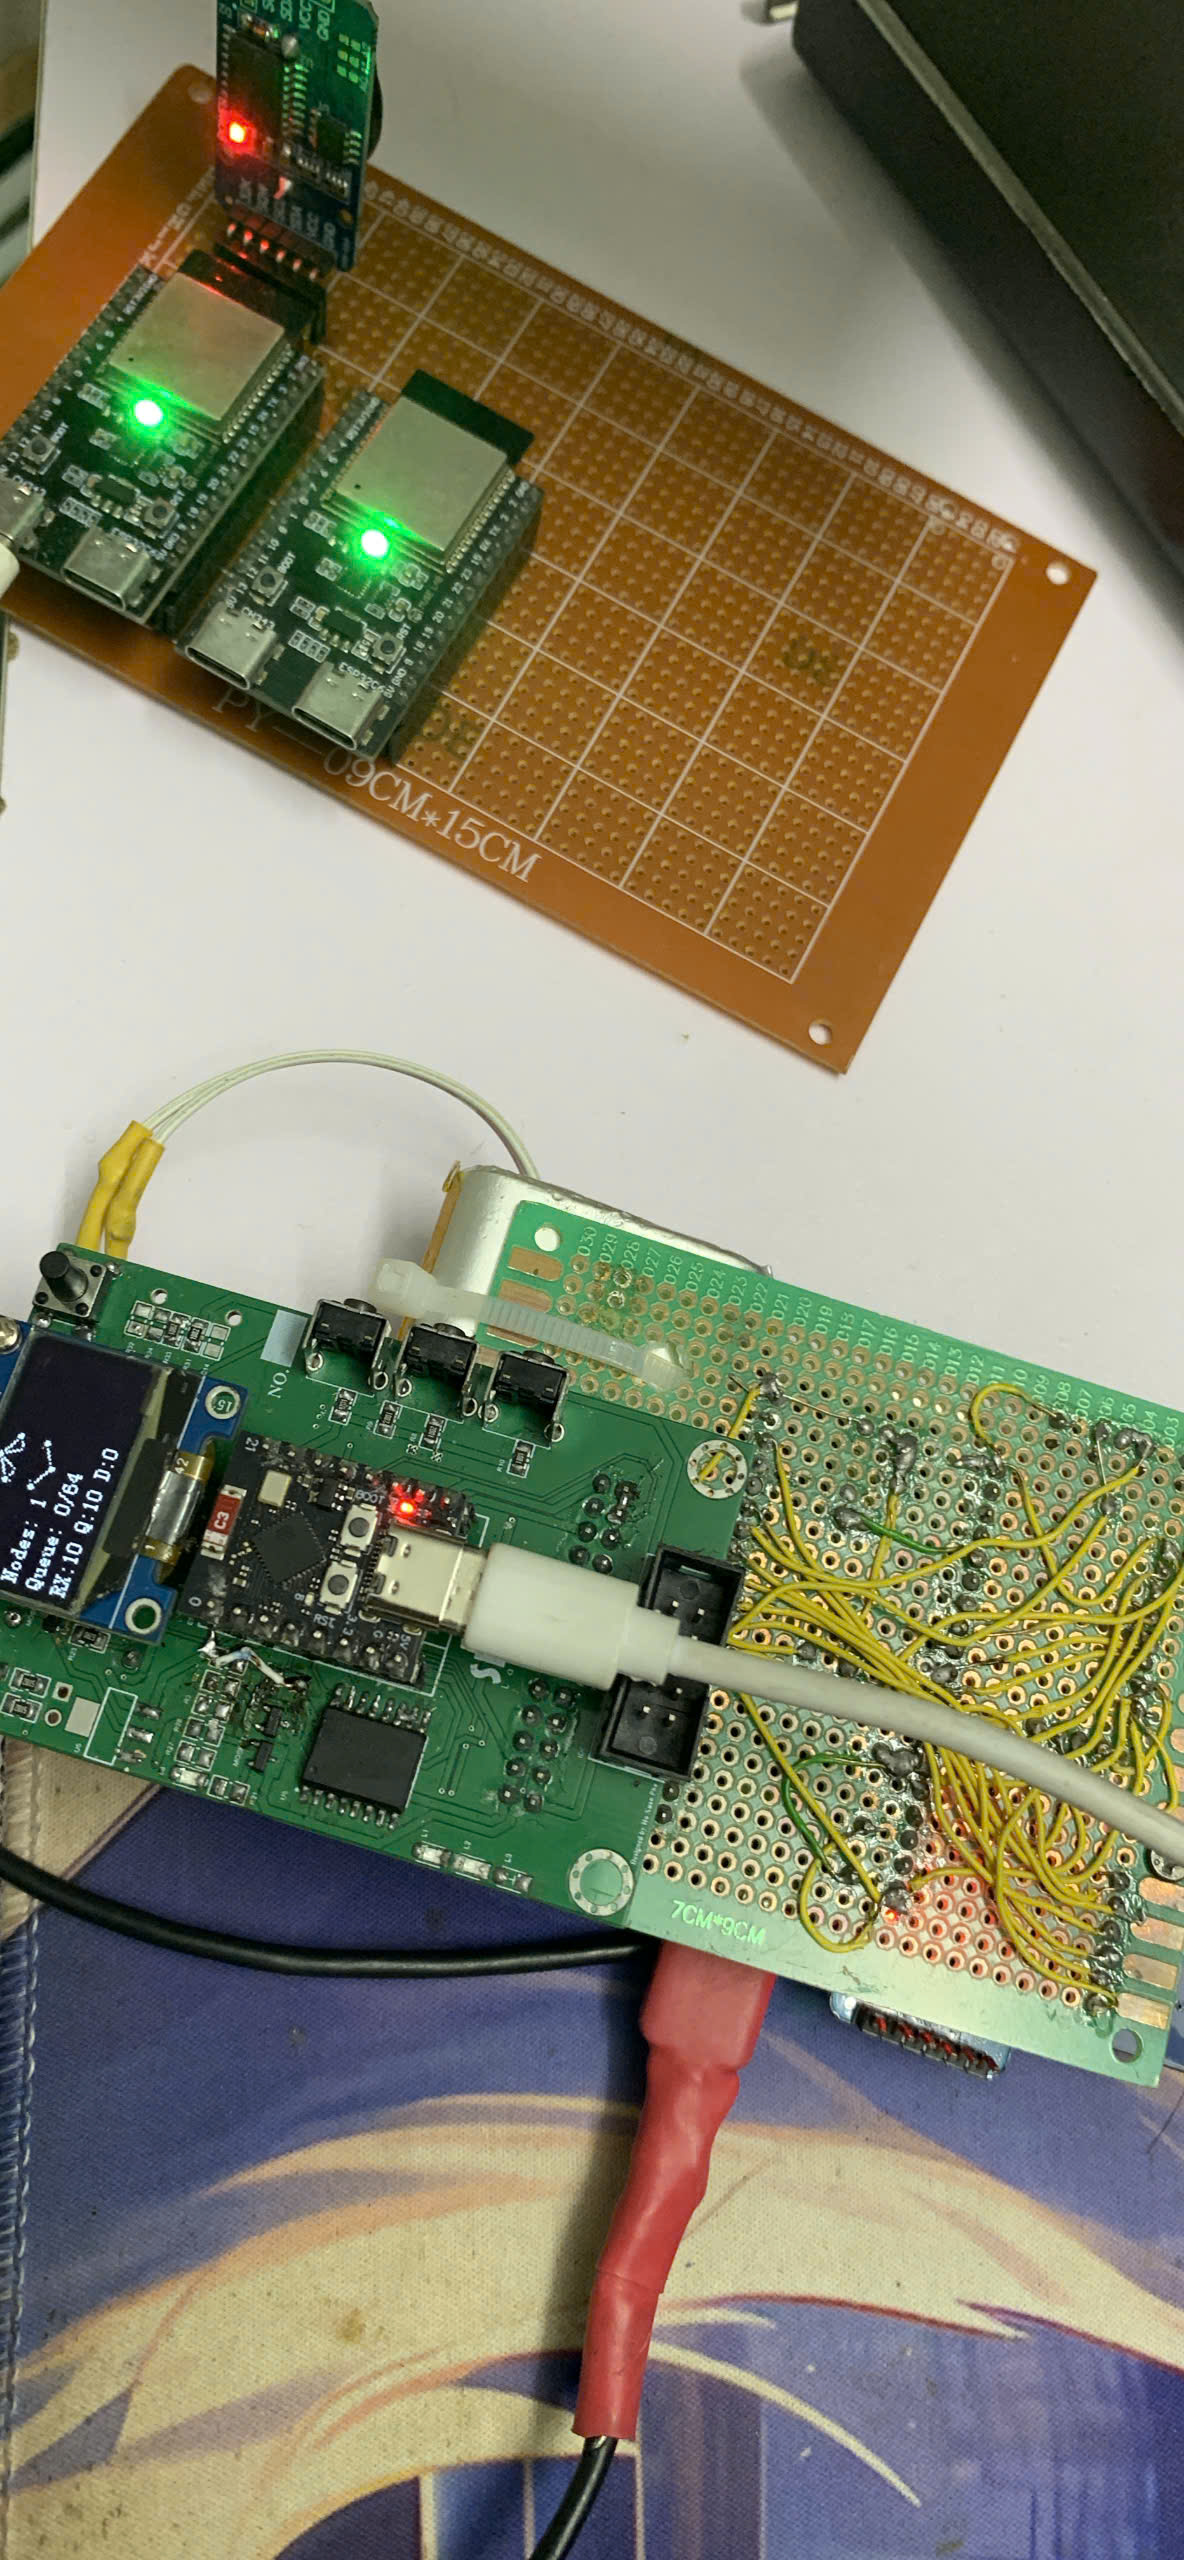
\includegraphics[width=\linewidth]{Images/setup3.jpg}
        \caption*{Kết nối toàn hệ thống}
    \end{minipage}
    \caption{Bố trí thiết lập môi trường kiểm thử thực tế (End-to-End).}
    \label{fig:setup}
\end{figure}

Dữ liệu thu thập từ các Node MSMS và Gateway được truyền xuyên suốt lên Server và thể hiện trực quan trên Web Dashboard. Các hình ảnh dưới đây minh chứng cho việc hệ thống đã gửi thông luồng dữ liệu lên tới giao diện người dùng và tệp tin log một cách đầy đủ và chính xác:

\begin{figure}[H]
    \centering
    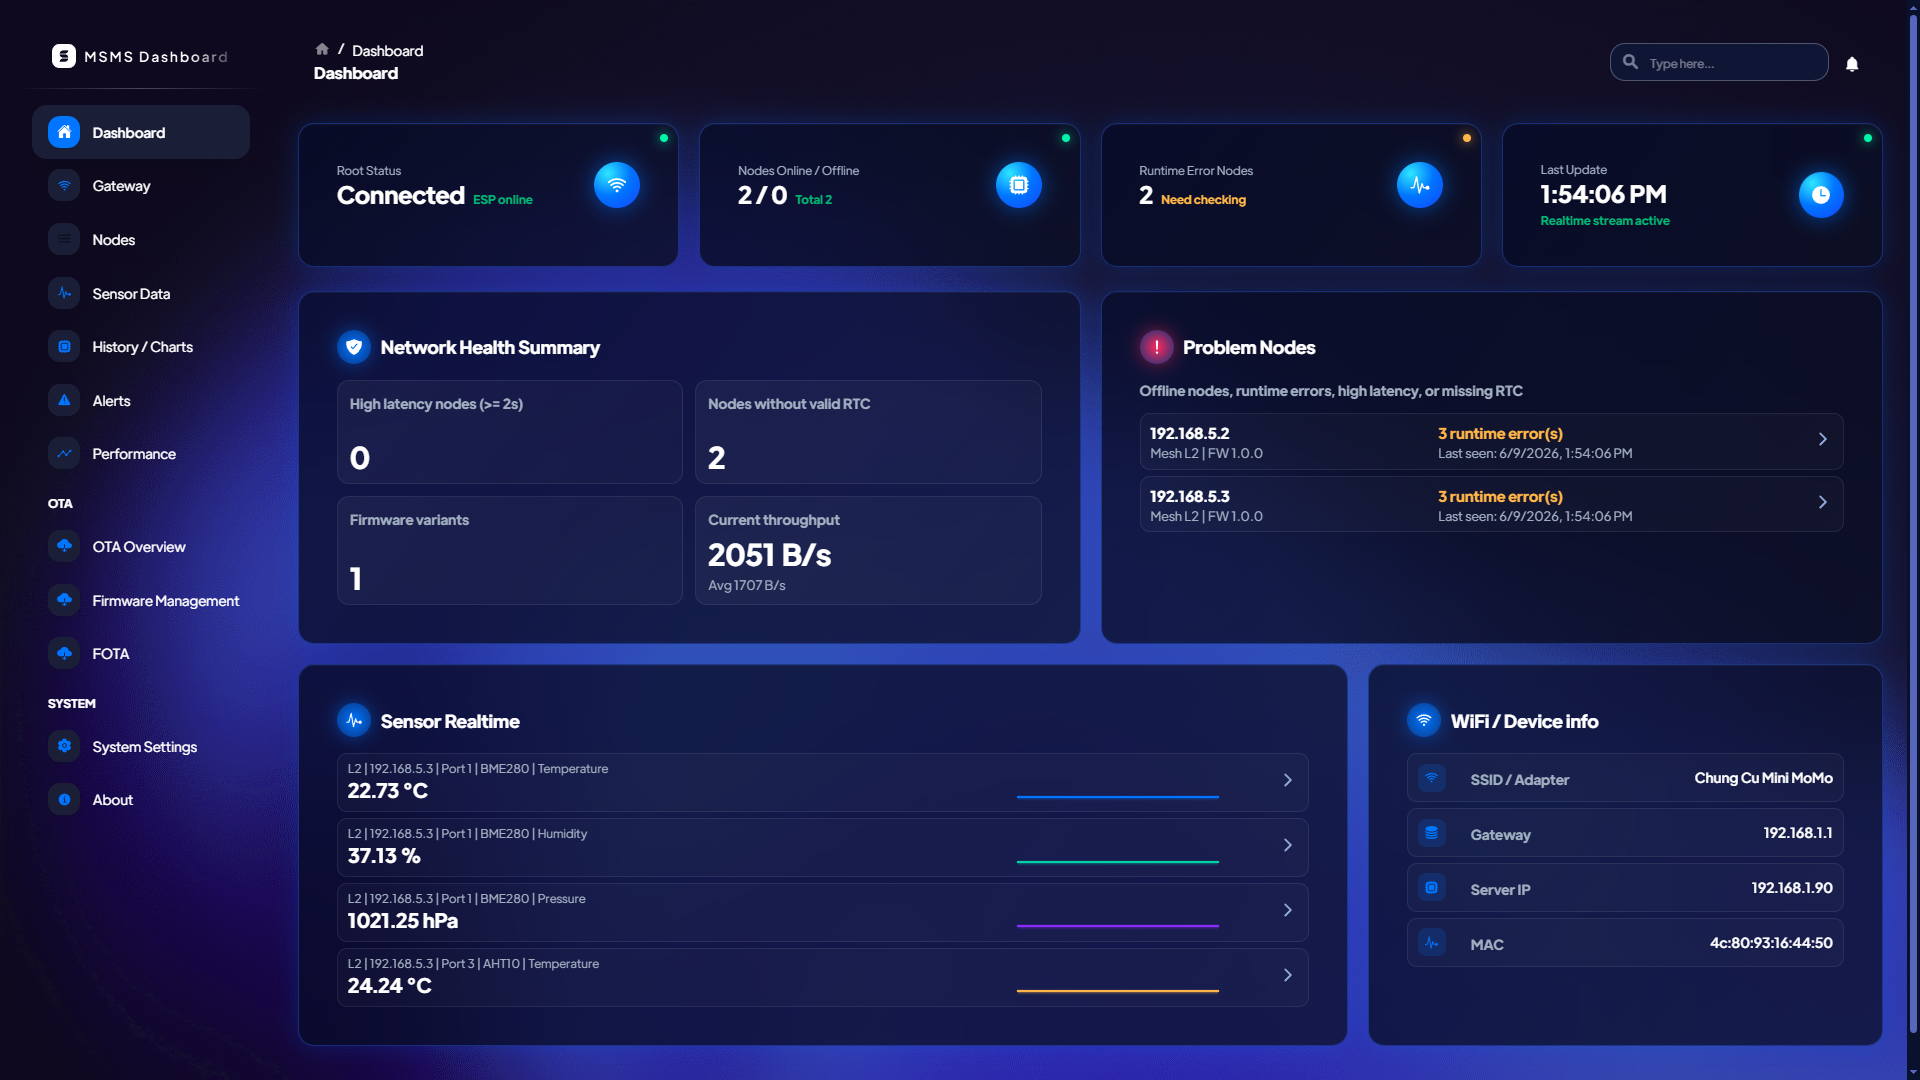
\includegraphics[width=0.8\textwidth]{Images/Main Dashboard.png}
    \caption{Giao diện tổng quan (Main Dashboard) của Server hiển thị bản đồ và số liệu.}
\end{figure}

\begin{figure}[H]
    \centering
    \begin{minipage}[t]{0.48\textwidth}
        \centering
        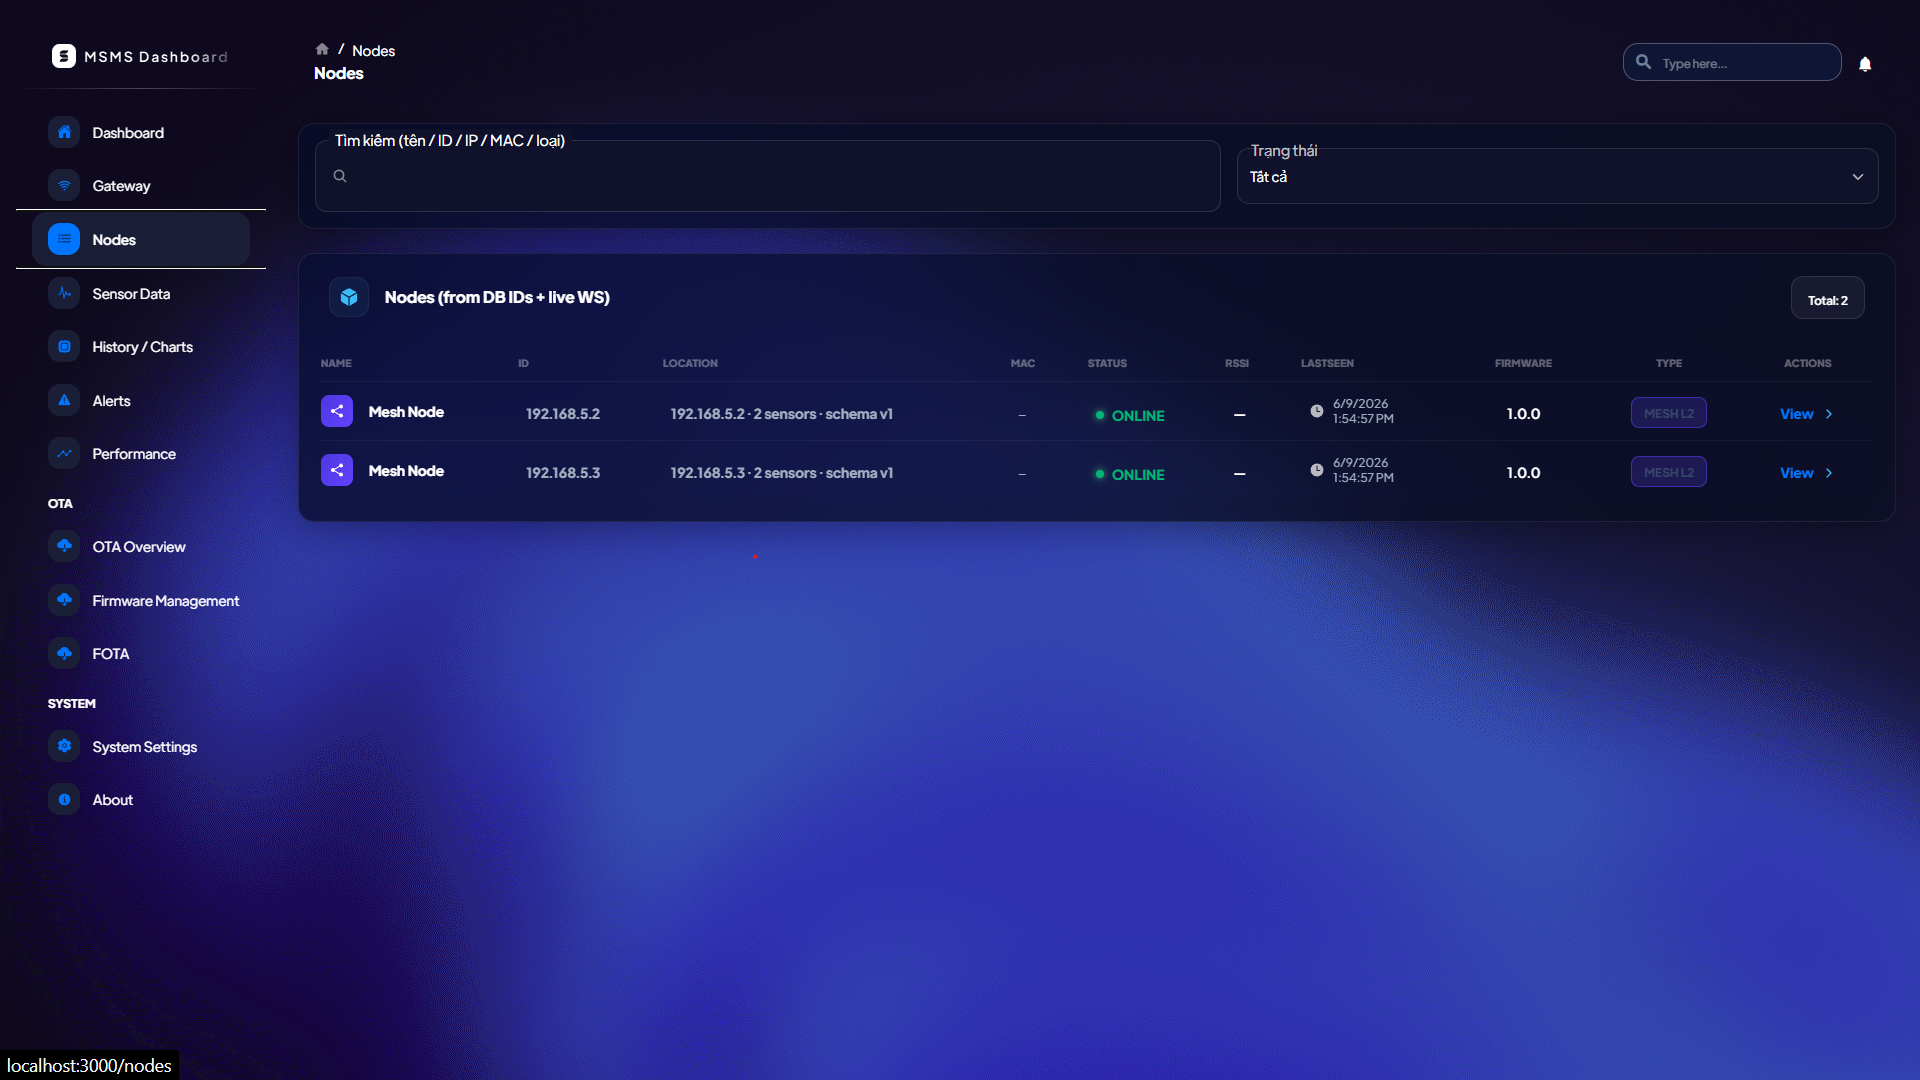
\includegraphics[width=\linewidth]{Images/Node Dashboard.png}
        \caption{Danh sách các Node đang hoạt động.}
    \end{minipage}\hfill
    \begin{minipage}[t]{0.48\textwidth}
        \centering
        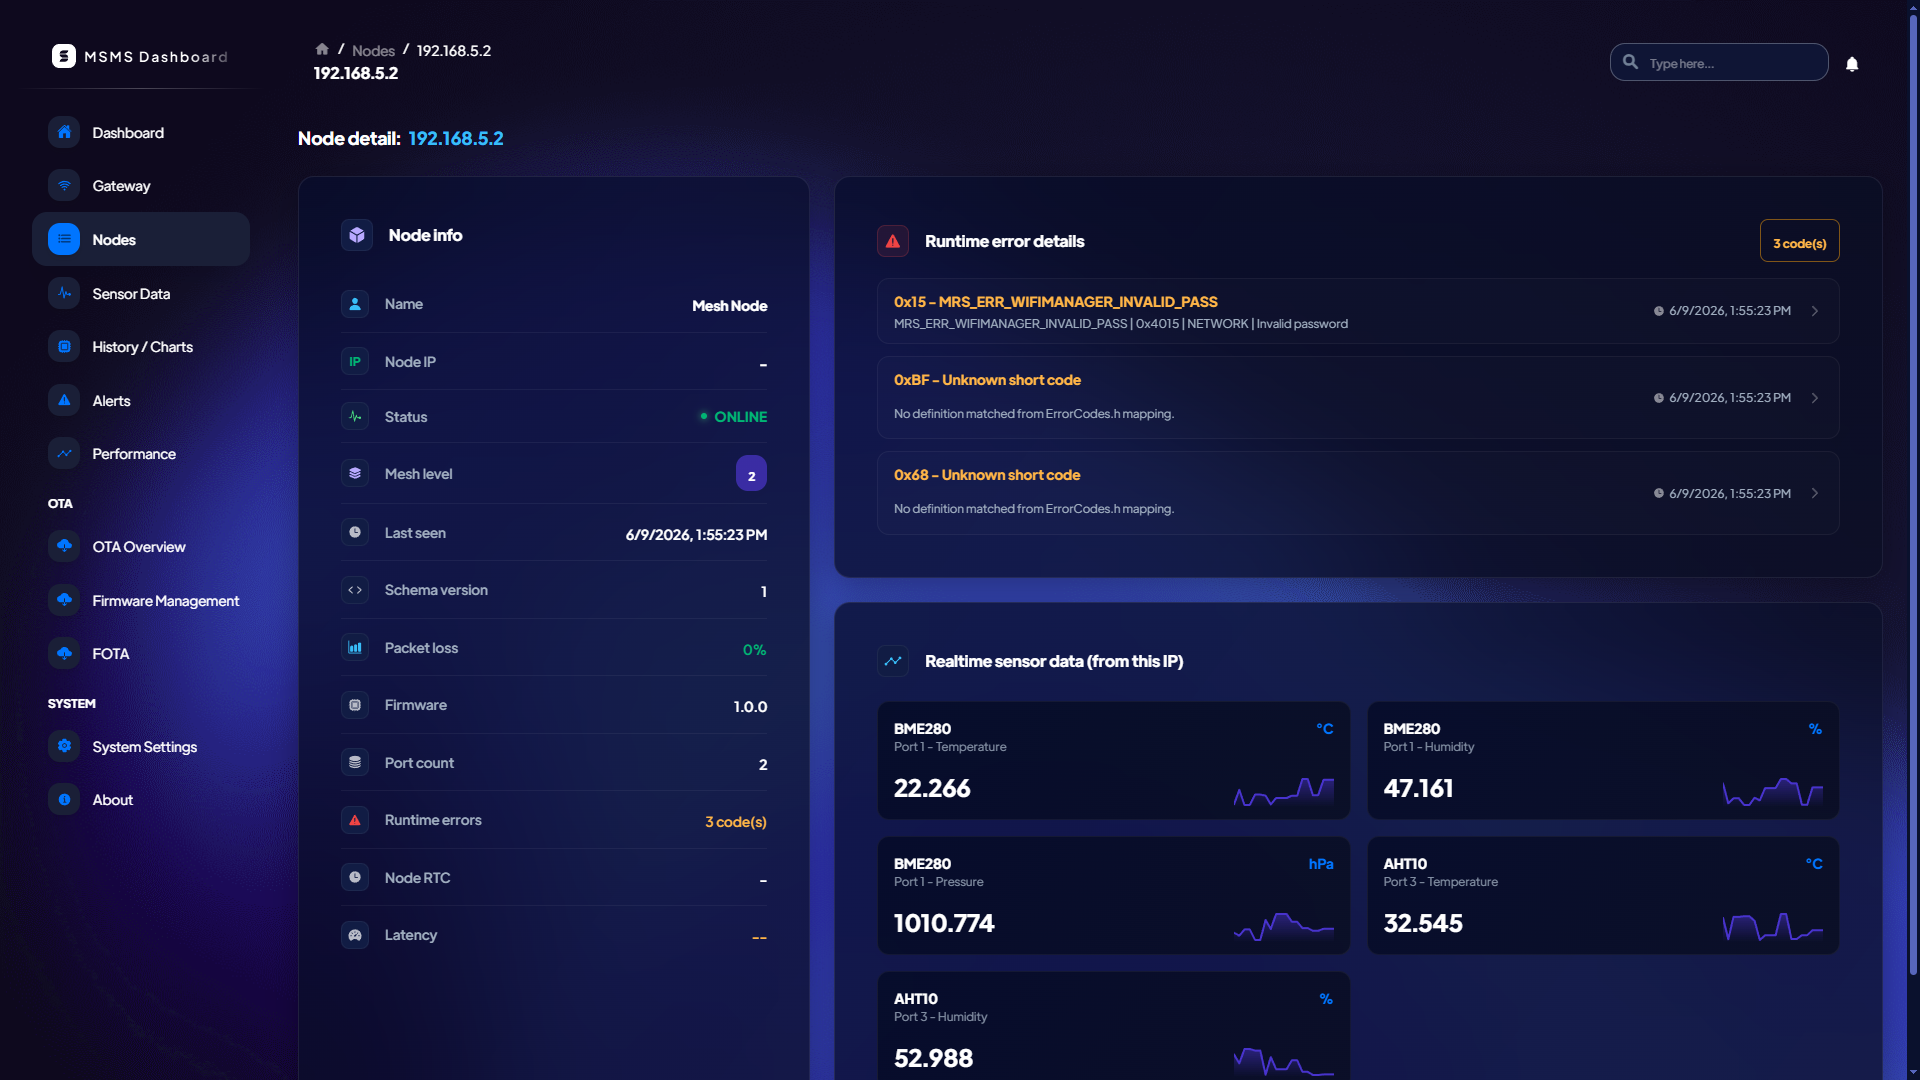
\includegraphics[width=\linewidth]{Images/NodeDetailDashboard.png}
        \caption{Chi tiết dữ liệu đo đạc của một Node.}
    \end{minipage}
\end{figure}

\begin{figure}[H]
    \centering
    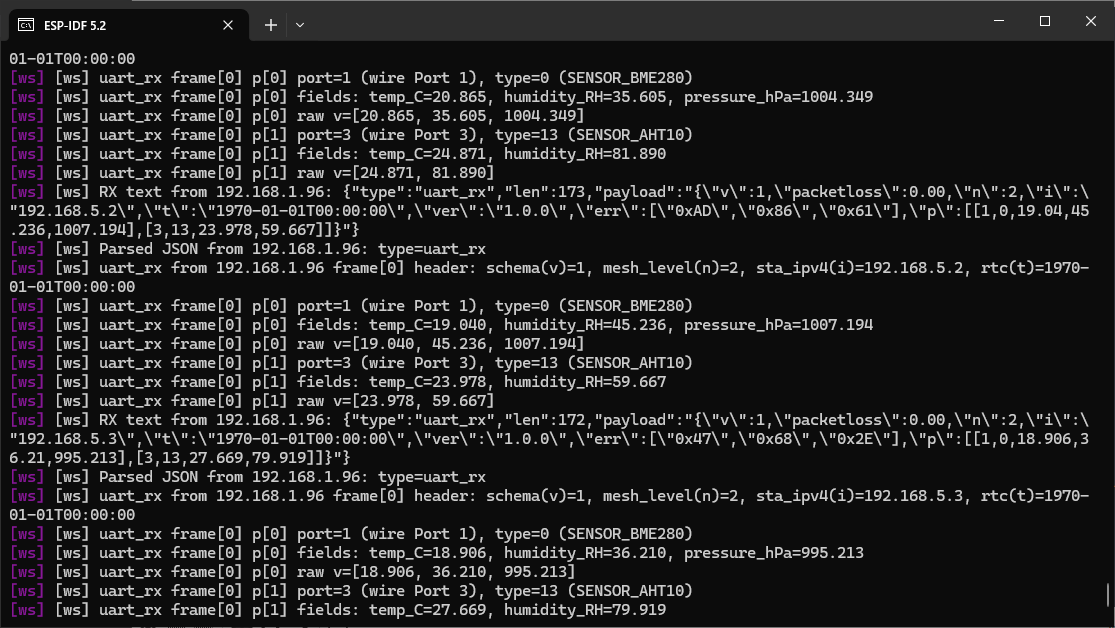
\includegraphics[width=0.8\textwidth]{Images/logData.png}
    \caption{Cơ sở dữ liệu lưu lại log lịch sử đo đạc từ các Node.}
\end{figure}

\subsection{Đánh giá hiệu năng mạng Mesh (Packet Loss)}

Để chứng minh độ ổn định của mạng Wi-Fi Mesh-Lite dưới cường độ cao, một bài kiểm tra suy hao gói tin (Packet Loss) đã được thực hiện. Hai Node MSMS đồng thời phát liên tục các gói tin về ROOT Node để chuyển tiếp lên máy chủ, với 2 tần suất thử nghiệm:
\begin{itemize}
    \item \textbf{Tần suất 10Hz} (chu kỳ gửi 100ms/gói).
    \item \textbf{Tần suất 100Hz} (chu kỳ gửi 10ms/gói).
\end{itemize}

Kết quả thu được thông qua theo dõi trên máy chủ (hiển thị ở Hình~\ref{fig:pkl}) cho thấy hệ thống hoạt động vô cùng ổn định: tỷ lệ mất gói tin (Packet Loss) hoàn toàn bằng \textbf{0\%} ở cả hai tần suất lấy mẫu, chứng tỏ cấu trúc mạng và năng lực xử lý của Gateway đáp ứng rất tốt môi trường công nghiệp yêu cầu tốc độ cập nhật siêu cao.

\begin{figure}[H]
    \centering
    \begin{minipage}[t]{0.48\textwidth}
        \centering
        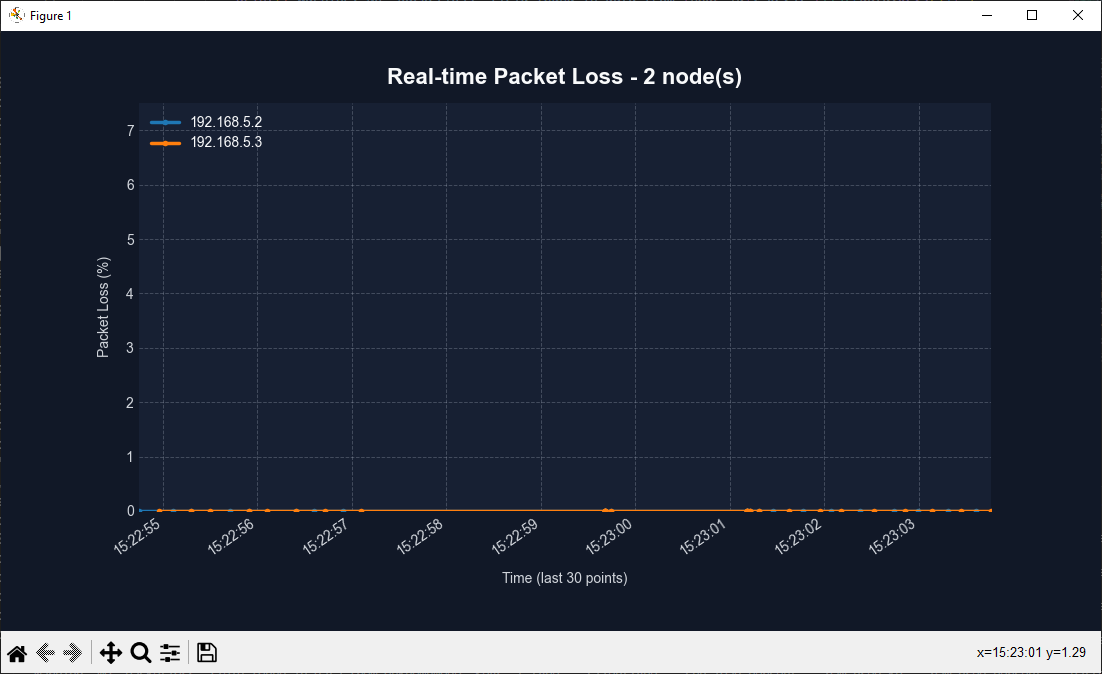
\includegraphics[width=\linewidth]{Images/PKL_10ms.png}
        \caption{Hiệu suất khi truyền dữ liệu 10Hz (Packet loss = 0\%).}
    \end{minipage}\hfill
    \begin{minipage}[t]{0.48\textwidth}
        \centering
        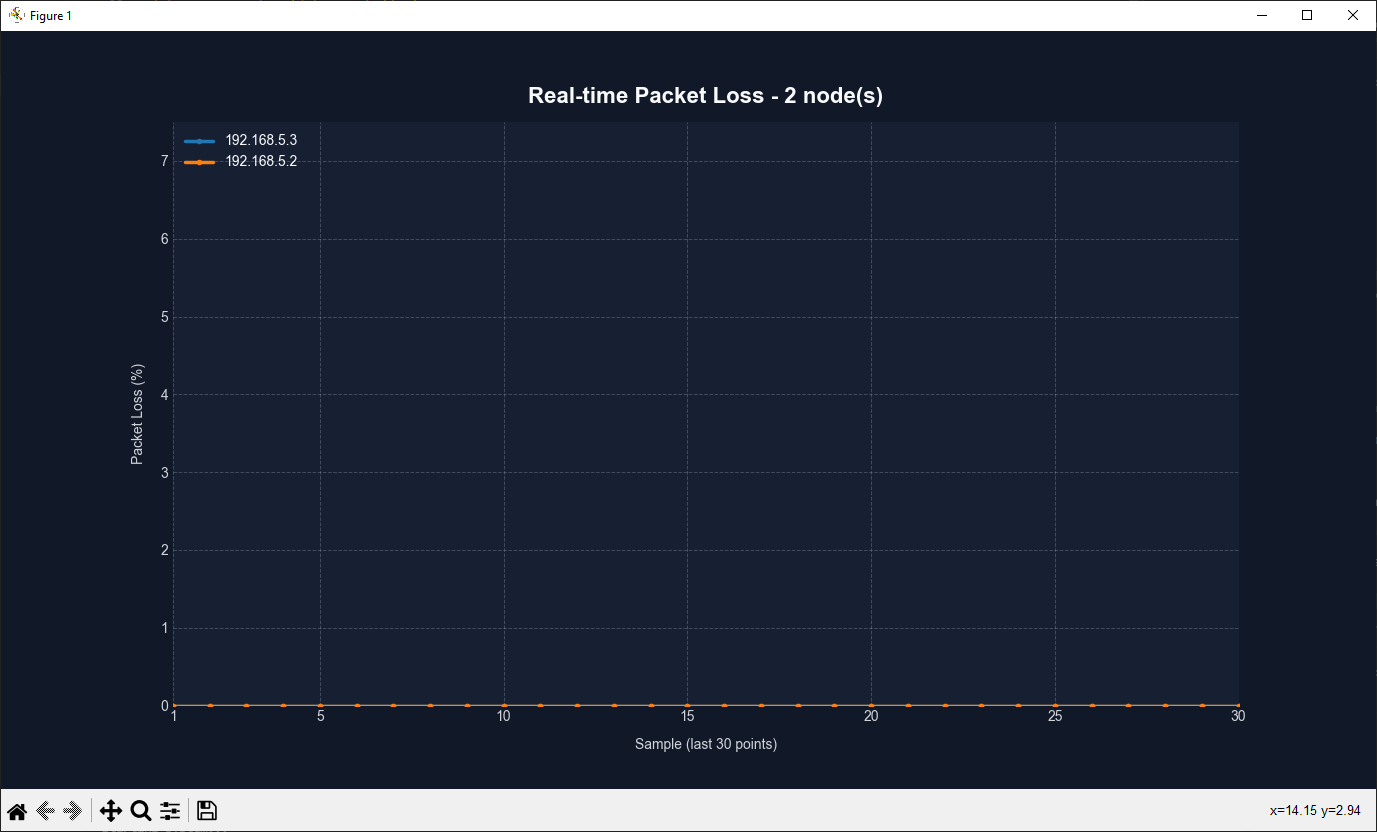
\includegraphics[width=\linewidth]{Images/PKL_100hz.png}
        \caption{Hiệu suất khi truyền dữ liệu 100Hz (Packet loss = 0\%).}
    \end{minipage}
    \caption{Kết quả kiểm tra suy hao gói tin mạng Wi-Fi Mesh.}
    \label{fig:pkl}
\end{figure}

\subsection{Tổng hợp kết quả kiểm thử}

Bảng~\ref{tab:test_summary} tóm tắt kết quả kiểm thử toàn diện của hệ thống:

\begin{table}[H]
    \centering
    \caption{Tóm tắt kết quả kiểm thử hệ thống tổng thể}
    \label{tab:test_summary}
    \small
    \resizebox{\textwidth}{!}{%
    \begin{tabular}{|l|l|c|}
        \hline
        \textbf{Nhóm kiểm thử} & \textbf{Nội dung chính} & \textbf{Kết quả} \\
        \hline
        Phần cứng MSMS & Nguồn 3.3V/5V ổn định, Nút bấm nhạy, OLED I2C ổn định & Đạt \\
        \hline
        Firmware MSMS & Mesh-Lite Role Switch tốt, gửi UDP không nghẽn mạng & Đạt \\
        \hline
        Phần cứng Gateway & TFT LVGL vẽ mượt 30fps, RTC chạy ngầm, thẻ SD lưu tốt & Đạt \\
        \hline
        Firmware Gateway & Phân tích cJSON tốc độ cao, giao tiếp UART không mất gói & Đạt \\
        \hline
        Web \& Server & Node.js \& MongoDB chịu tải cao, Web Dashboard Real-time tốt & Đạt \\
        \hline
        Mobile App & React Native đồng bộ dữ liệu nhanh, UI/UX mượt mà & Đạt \\
        \hline
        Tích hợp toàn hệ thống & Luồng truyền tải End-to-End xuyên suốt, độ trễ $<500$ms & Đạt \\
        \hline
    \end{tabular}%
    }
\end{table}
\newpage

\section*{CHƯƠNG 5. KẾT LUẬN VÀ HƯỚNG PHÁT TRIỂN}
\addcontentsline{toc}{section}{\numberline{}CHƯƠNG 5. KẾT LUẬN VÀ HƯỚNG PHÁT TRIỂN}
\setcounter{section}{5}
\setcounter{subsection}{0}
\setcounter{figure}{0}
\setcounter{table}{0}
\subsection{Kết quả đạt được}
Dự án \textbf{Hệ thống quản lý cảm biến đa năng mạng Wi-Fi Mesh (MSMS)} đã hoàn thành thiết kế, chế tạo phần cứng và phát triển toàn diện hệ sinh thái phần mềm từ thiết bị đầu cuối đến máy chủ và ứng dụng người dùng. Cụ thể:
\begin{itemize}
    \item \textbf{Mạch Node MSMS}: Chế tạo thành công thiết bị đo đạc với ESP32, màn hình OLED, nút bấm và cảm biến mở rộng. Firmware tích hợp cấu trúc phân lớp FreeRTOS, hỗ trợ tự động định tuyến mạng ESP-Mesh-Lite và gửi dữ liệu UDP tốc độ cao.
    \item \textbf{Mạch Gateway (Trạm thu thập)}: Chế tạo thành công bộ điều khiển trung tâm với màn hình TFT cảm ứng chạy LVGL, tích hợp đồng hồ RTC DS3231 và ghi log thẻ nhớ SD. Gateway làm nhiệm vụ ROOT Node, gom dữ liệu Mesh và chuyển tiếp mượt mà lên Server thông qua WebSocket.
    \item \textbf{Web Dashboard \& Mobile App}: Xây dựng thành công máy chủ Node.js/MongoDB để lưu trữ dữ liệu lịch sử. Giao diện Web (React.js) và ứng dụng di động (React Native) hoạt động ổn định, vẽ đồ thị Real-time sắc nét, mang lại trải nghiệm người dùng hiện đại và tiện lợi.
    \item \textbf{Tích hợp toàn hệ thống}: Hệ thống đã vượt qua các bài kiểm thử End-to-End khắt khe. Dữ liệu từ cảm biến vật lý truyền xuyên suốt qua mạng Mesh, qua Gateway, lên Cloud và đến thiết bị người dùng cuối với độ trễ rất thấp (chỉ dưới 500ms).
\end{itemize}

\subsection{Hướng phát triển}
Hệ thống hiện tại đã hoạt động ổn định như một mạng lưới IoT hoàn chỉnh. Trong tương lai, dự án có thể được mở rộng theo các hướng:

\textbf{1. Đa dạng hóa Node Cảm biến và Cơ cấu chấp hành:}
\begin{itemize}
    \item Mở rộng thêm các Node chuyên dụng đo \textbf{chất lượng không khí công nghiệp} (VOC, O3, NO2, SO2).
    \item Bổ sung các Node \textbf{Actuator} (Cơ cấu chấp hành) như rơ-le thông minh để tự động bật quạt hút, bơm nước hoặc kích hoạt chuông báo động dựa trên luồng dữ liệu theo thời gian thực phân tích từ Server.
\end{itemize}

Về mặt công nghệ, hệ thống sẽ được nâng cấp với các tính năng:
\begin{itemize}
    \item \textbf{Trí tuệ nhân tạo (AI):} Ứng dụng machine learning để dự báo chất lượng không khí dựa trên dữ liệu lịch sử và các yếu tố môi trường như thời tiết, giao thông, hoạt động công nghiệp.
    \item \textbf{Mạng lưới quan trắc:} Kết nối nhiều trạm quan trắc tại các vị trí khác nhau để tạo thành mạng lưới giám sát chất lượng không khí trên diện rộng, cho phép vẽ bản đồ ô nhiễm không khí theo thời gian thực.
    \item \textbf{Tích hợp dữ liệu thời tiết:} Kết nối với các API thời tiết để phân tích mối quan hệ giữa điều kiện thời tiết và chất lượng không khí.
    \item \textbf{Cảnh báo thông minh:} Phát triển hệ thống cảnh báo thông minh dựa trên AI để dự đoán các đợt ô nhiễm không khí và gửi cảnh báo sớm đến người dùng.
\end{itemize}

Về mặt ứng dụng, hệ thống có thể được mở rộng để:
\begin{itemize}
    \item \textbf{Tích hợp với ứng dụng di động:} Phát triển ứng dụng mobile để người dùng có thể theo dõi chất lượng không khí mọi lúc mọi nơi và nhận cảnh báo khi cần thiết.
    \item \textbf{Phân tích dữ liệu nâng cao:} Xây dựng các dashboard phân tích với khả năng so sánh dữ liệu giữa các thời điểm, các khu vực và đưa ra các khuyến nghị về sức khỏe.
    \item \textbf{Tích hợp với hệ thống quản lý môi trường:} Kết nối với các hệ thống quản lý môi trường của cơ quan nhà nước để đóng góp dữ liệu vào hệ thống giám sát quốc gia.
\end{itemize}

Về mặt kỹ thuật, với nguồn lực tài chính được cải thiện trong tương lai, hệ thống có thể được nâng cấp:
\begin{itemize}
    \item \textbf{Cảm biến chất lượng cao hơn:} Thay thế các cảm biến hiện tại bằng các cảm biến chuyên nghiệp có độ chính xác và độ bền cao hơn, đáp ứng các tiêu chuẩn quốc tế về quan trắc môi trường.
    \item \textbf{Nguồn năng lượng:} Tích hợp pin mặt trời để hệ thống có thể hoạt động hoàn toàn độc lập trong thời gian dài.
    \item \textbf{Truyền dữ liệu:} Mở rộng khả năng truyền dữ liệu bằng cách tích hợp thêm các công nghệ như LoRa, NB-IoT để đảm bảo kết nối ổn định ở các khu vực xa xôi.
    \item \textbf{Bảo vệ môi trường:} Thiết kế vỏ bảo vệ chống bụi, chống nước để hệ thống có thể hoạt động ổn định trong các điều kiện môi trường khắc nghiệt.
\end{itemize}



\newpage

\phantomsection
\addcontentsline{toc}{section}{\numberline {}TÀI LIỆU THAM KHẢO} % Thêm TÀI LIỆU THAM KHẢO vào mục lục
\nocite{*}
\bibliographystyle{IEEEtran}  % Định dạng tham khảo
\bibliography{TaiLieuThamKhao}  % Đường dẫn đến tệp .bib
\end{document}

